%  PROYECTO DE INNOVACIÓN Y/O MEJORA - Formato SENATI (modelo del asesor + metodología PIM)
% ------------------------------------------------------------------------------------------
% Formato tomado del modelo G4_MODELO: Times 12 pt, doble espacio, sangría de primera línea,
% encabezado corto (máx. 5 palabras) en cursiva, número de página centrado al pie,
% capítulos en página propia, tablas y figuras estilo APA con "Nota." al pie.

\documentclass[12pt,a4paper]{report}

% ---------- Idioma y codificación ----------
\usepackage[utf8]{inputenc}
\usepackage[T1]{fontenc}
\usepackage[spanish,es-tabla]{babel}
\usepackage{float}
\decimalpoint

% ---------- Tipografía estilo Times ----------
\usepackage{mathptmx}

% ---------- Márgenes de 2.54 cm (1 pulgada), como el modelo ----------
\usepackage[a4paper,margin=2.54cm]{geometry}

% ---------- Interlineado doble (el modelo usa doble espacio) ----------
\usepackage{setspace}
\setstretch{1.9}
\setlength{\parindent}{1.25cm}
\setlength{\parskip}{0pt}

% ---------- Color (para marcar pendientes) ----------
\usepackage[table]{xcolor}
\definecolor{pendcol}{RGB}{192,0,0}
\definecolor{headgray}{gray}{0.45}

% ---------- Encabezado (5 palabras como máximo) y pie de página ----------
\usepackage{fancyhdr}
\newcommand{\titulocorto}{Sistema web de gestión tributaria}
\pagestyle{fancy}
\setlength{\headheight}{14.5pt}
\fancyhf{}
\fancyhead[L]{\small\itshape\color{headgray}\titulocorto}
\fancyfoot[C]{\thepage}
\renewcommand{\headrulewidth}{0pt}
\fancypagestyle{plain}{%
  \fancyhf{}
  \fancyhead[L]{\small\itshape\color{headgray}\titulocorto}
  \fancyfoot[C]{\thepage}
  \renewcommand{\headrulewidth}{0pt}
}

% ---------- Otros paquetes ----------
\usepackage{graphicx}
\usepackage{tikz}
\usetikzlibrary{positioning,shapes.geometric,arrows.meta,fit,patterns}
\usepackage[font=normalsize]{caption}
\usepackage{booktabs}
\usepackage{longtable}
\usepackage{array}
\newcolumntype{L}[1]{>{\raggedright\arraybackslash}p{#1}}
\usepackage{enumitem}
\usepackage{amsmath,amssymb}
% Fragmentos de código (Capítulo IV)
\usepackage{listings}
\lstset{basicstyle=\setstretch{1}\ttfamily\scriptsize, breaklines=true, frame=single,
  columns=fullflexible, keepspaces=true, showstringspaces=false, xleftmargin=2em, framexleftmargin=1.6em, numbersep=6pt,
  numbers=left, numberstyle=\tiny\color{headgray}, keywordstyle=\bfseries, commentstyle=\itshape\color{headgray},
  literate={á}{{\'a}}1 {é}{{\'e}}1 {í}{{\'i}}1 {ó}{{\'o}}1 {ú}{{\'u}}1 {ñ}{{\~n}}1
           {Á}{{\'A}}1 {É}{{\'E}}1 {Í}{{\'I}}1 {Ó}{{\'O}}1 {Ú}{{\'U}}1}
\usepackage[hidelinks]{hyperref}
\usepackage{csquotes}
\usepackage[
  backend=biber,
  style=apa,
  sorting=nyt
]{biblatex}
\DeclareLanguageMapping{spanish}{spanish-apa} % APA en español ("y", "s.f.", etc.)
\addbibresource{referencias.bib}
% Permite cortar los DOI/URL largos sin abrir espacios entre caracteres
\setcounter{biburlnumpenalty}{100}
\setcounter{biburlucpenalty}{100}
\setcounter{biburllcpenalty}{100}
\biburlbigskip=0mu plus 0.5mu
\biburlnumskip=0mu plus 0.5mu
\biburlucskip=0mu plus 0.5mu
\biburllcskip=0mu plus 0.5mu

\graphicspath{{imagenes/}}

% Diagramas BPMN: si existe imagenes/bizagi_<nombre>.png (exportado desde Bizagi Modeler) se usa ese;
% si no, se usa imagenes/bpmn_<nombre>.pdf (generado con bizagi/generar_bpmn.py).
\usepackage{rotating}
\newcommand{\diagrama}[2]{\IfFileExists{imagenes/bizagi_#1.png}{\includegraphics[width=#2]{bizagi_#1.png}}{\includegraphics[width=#2]{bpmn_#1.pdf}}}


% Inserta la imagen si existe; si no, muestra un recuadro marcador (no rompe la compilación)
\newcommand{\imgopt}[2]{%
  \IfFileExists{imagenes/#2}{\includegraphics[width=#1\textwidth]{#2}}%
  {\fbox{\parbox[c][4cm][c]{0.6\textwidth}{\centering\textit{[Insertar imagen: \detokenize{#2}]}}}}%
}

% ---------- Numeración "1.1." / "1.1.1." y títulos como el modelo ----------
\setcounter{secnumdepth}{3}
\setcounter{tocdepth}{3}
\usepackage{titlesec}
% Capítulo: "CAPÍTULO I" + título, centrado, en página propia (como el modelo)
\titleformat{\chapter}[display]
  {\vspace*{0.28\textheight}\centering\bfseries\large}
  {\MakeUppercase{\chaptername}\ \Roman{chapter}}{0pt}
  {\MakeUppercase}[\clearpage]
% Capítulo sin número (Agradecimiento, Resumen, Introducción, Anexos...)
\titleformat{name=\chapter,numberless}[block]
  {\centering\bfseries\normalsize}{}{0pt}{\MakeUppercase}
\titlespacing*{\chapter}{0pt}{0pt}{6pt}
\titleformat{\section}{\bfseries\normalsize}{\thesection.}{0.6em}{}
\titleformat{\subsection}{\bfseries\itshape\normalsize}{\thesubsection.}{0.6em}{}
\titleformat{\subsubsection}{\itshape\normalsize}{\thesubsubsection.}{0.6em}{}
\titlespacing*{\section}{0pt}{8pt}{0pt}
\titlespacing*{\subsection}{0pt}{6pt}{0pt}
\titlespacing*{\subsubsection}{1.25cm}{6pt}{0pt}

% Índice: "Capítulo 1 ..."
\usepackage{tocloft}
\renewcommand{\cftchappresnum}{Capítulo~}
\setlength{\cftchapnumwidth}{5.2em}
\renewcommand{\cftdotsep}{1.5}
\renewcommand{\cftchapdotsep}{\cftdotsep}
\setlength{\cftbeforechapskip}{4pt}
% Títulos de los índices: centrados, mayúsculas y negrita (como los demás capítulos sin número)
\renewcommand{\cfttoctitlefont}{\hfill\bfseries\normalsize}
\renewcommand{\cftaftertoctitle}{\hfill}
\renewcommand{\cftloftitlefont}{\hfill\bfseries\normalsize}
\renewcommand{\cftafterloftitle}{\hfill}
\renewcommand{\cftlottitlefont}{\hfill\bfseries\normalsize}
\renewcommand{\cftafterlottitle}{\hfill}
\setlength{\cftbeforetoctitleskip}{0pt}
\setlength{\cftbeforeloftitleskip}{0pt}
\setlength{\cftbeforelottitleskip}{0pt}

% ---------- Tablas y figuras estilo APA: "Tabla 1" (negrita) / título en cursiva / Nota. ----------
\usepackage{chngcntr}
\counterwithout{table}{chapter}   % numeración continua: Tabla 1, Tabla 2...
\counterwithout{figure}{chapter}
\renewcommand{\thetable}{\arabic{table}}
\renewcommand{\thefigure}{\arabic{figure}}
\captionsetup{labelfont=bf,textfont=it,labelsep=newline,singlelinecheck=false,justification=raggedright,skip=3pt}
\captionsetup[figure]{justification=centering}
\setlength{\intextsep}{10pt}

% "Nota." al pie de cada tabla o figura, pegada a la imagen (observación del asesor:
% "no separar tanto la imagen con la nota")
\newcommand{\nota}[1]{\par\vspace{1pt}{\singlespacing\footnotesize\raggedright\textit{Nota.} #1\par}}

% Dato aún por completar (se ve en rojo; búscalo con "Pendiente")
\newcommand{\pend}[1]{\textcolor{pendcol}{[Pendiente: #1]}}

% Valor provisional (supuesto) que debe validarse con la empresa o la municipalidad.
% Se imprime en rojo para que se distinga a simple vista.
\newcommand{\supuesto}[1]{\textcolor{pendcol}{#1}}

% Causas con estilo "a) Nombre ..." en cursiva y SIN negrita (observación del asesor)
\newcommand{\causa}[2]{\par\textit{#1)~#2}.\ }

% Rojo usado en el organigrama para resaltar a los usuarios del sistema (metodología PIM, hoja 1.4)
\definecolor{rojopim}{RGB}{192,0,0}

% ---------- Cálculo automático de pérdidas, costos y beneficio (Capítulos III, V y VI) ----------
% Cambia SOLO estos valores cuando tengas los datos reales: todas las tablas se recalculan.
% Los valores marcados como SUPUESTO se imprimen en rojo en el PDF.
\usepackage{xfp}
\usepackage{pgfmath,pgfkeys}
\pgfkeys{/pgf/number format/.cd,fixed,fixed zerofill,precision=2,1000 sep={\mbox{,}}}
\newcommand{\setval}[2]{\edef#1{\fpeval{#2}}}
\newcommand{\soles}[1]{\edef\tmpval{\fpeval{round(#1,2)}}S/~\pgfmathprintnumber{\tmpval}}
\newcommand{\dolares}[1]{\edef\tmpval{\fpeval{round(#1,2)}}\$~\pgfmathprintnumber{\tmpval}}
\newcommand{\num}[2][2]{{\edef\tmpval{\fpeval{round(#2,#1)}}\pgfkeys{/pgf/number format/precision=#1}\pgfmathprintnumber{\tmpval}}}
% Parámetros generales
\setval{\RMV}{1230}            % D.S. 015-2026-TR
\setval{\HorasMes}{240}         % 30 días x 8 horas
\setval{\ValorHora}{\RMV/\HorasMes}
% ===== Capítulo III: pérdidas =====
% Causa a) Falta de estandarización
\setval{\VersionesAnio}{35/6}   % 35 versiones entre 2020 y 2025 (medido)
\setval{\MuniAdicionales}{3}    % SUPUESTO: otras municipalidades con su propia copia
\setval{\HorasAdaptacion}{4}    % SUPUESTO: horas para adaptar una corrección a otra copia
% Causa b) Interfaz obsoleta
\setval{\AtencionesMes}{660}    % MEDIDO en Simun: atenciones en caja por mes, promedio 2022-2024 (659.7)
\setval{\MinActual}{16.47}      % Laulate (2025): consulta de deudas, sistema anterior
\setval{\MinWeb}{2.50}          % Laulate (2025): consulta de deudas, sistema web
% Causa c) Demoras en el soporte técnico
\setval{\HorasDevVersion}{4}    % SUPUESTO: horas del desarrollador por versión
\setval{\Colaboradores}{8}      % encuesta (Tabla de Pareto)
\setval{\HorasParadaVersion}{2} % SUPUESTO: horas de trabajo detenido por colaborador y versión
% Causa d) Acceso limitado a información estadística
\setval{\ListadosMes}{4}        % SUPUESTO: listados de cobranza armados a mano por mes
\setval{\HorasListado}{3}       % SUPUESTO: horas para armar y depurar cada listado
\setval{\CartasMes}{652}        % MEDIDO en Simun: valores (OP y RD) emitidos por mes, promedio 2022-2024 (651.5)
\setval{\CostoCarta}{1.50}      % SUPUESTO: impresión y notificación de un valor (S/)
\setval{\TasaCartaSinEfecto}{0.323} % MEDIDO en Simun: valores emitidos 2019-2023 que siguen pendientes (32.3 %)
% Resultados (no editar)
\setval{\PerdA}{\VersionesAnio*\MuniAdicionales*\HorasAdaptacion*\ValorHora/12}
\setval{\HorasB}{\AtencionesMes*(\MinActual-\MinWeb)/60}
\setval{\PerdB}{\HorasB*\ValorHora}
\setval{\HorasC}{\VersionesAnio/12*(\HorasDevVersion+\Colaboradores*\HorasParadaVersion)}
\setval{\PerdC}{\HorasC*\ValorHora}
\setval{\PerdDuno}{\ListadosMes*\HorasListado*\ValorHora}
\setval{\PerdDdos}{\CartasMes*\CostoCarta*\TasaCartaSinEfecto}
\setval{\PerdD}{\PerdDuno+\PerdDdos}
\setval{\PerdMes}{\PerdA+\PerdB+\PerdC+\PerdD}
\setval{\PerdAnio}{12*\PerdMes}
% ===== Capítulo V: costos (calculadoras del asesor: Depreciación y ConsumoLuz) =====
\setval{\TC}{3.452}             % tipo de cambio venta SUNAT/SBS del 06/11/2026
% 5.1 Materiales (servicios en la nube por 12 meses)
\setval{\VpsMesUSD}{6.49}       % Hostinger VPS KVM 1, plan de 12 meses (precio publicado nov. 2026), US$ por mes
\setval{\BdMesUSD}{25}          % Supabase Pro, US$ por mes (precio publicado 2026)
\setval{\MesesServicio}{12}
\setval{\CostoVps}{\VpsMesUSD*\TC*\MesesServicio}
\setval{\CostoBd}{\BdMesUSD*\TC*\MesesServicio}
\setval{\CostoMat}{\CostoVps+\CostoBd}
% 5.2 Mano de obra
\setval{\Desarrolladores}{2}
\setval{\DiasHechos}{41}        % días hábiles del 11/09/2026 al 07/11/2026 (historial del repositorio)
\setval{\DiasPorHacer}{30}      % cronograma: días hábiles del 09/11 al 18/12/2026 (sprints 7 y 8)
\setval{\DiasDev}{\DiasHechos+\DiasPorHacer}
\setval{\CostoDia}{\RMV/30}     % jornal referencial = RMV / 30
\setval{\CostoMO}{\Desarrolladores*\DiasDev*\CostoDia}
% 5.3 Máquinas y equipos (depreciación lineal, fórmula del asesor)
\setval{\LaptopValor}{3000}     % SUPUESTO: valor inicial de cada laptop (S/)
\setval{\LaptopVida}{4}         % vida útil: 4 años (tasa máxima de 25 % anual para equipos de cómputo)
\setval{\LaptopResidual}{\LaptopValor/\LaptopVida}
\setval{\LaptopDeprec}{(\LaptopValor-\LaptopResidual)/\LaptopVida}
\setval{\CostoMaq}{\Desarrolladores*\LaptopDeprec}
% 5.4 Otros costos (consumo de luz e internet)
\setval{\Watts}{65}             % SUPUESTO: potencia de la laptop (W)
\setval{\HorasDia}{6}           % SUPUESTO: horas de programación por día
\setval{\Tarifa}{0.68}          % tarifa BT5B residencial de Lima, bloque 31-140 kWh (Osinergmin, abril 2026); confirmar con el recibo
\setval{\KwhMes}{\Watts/1000*\HorasDia*30}
\setval{\LuzMes}{\KwhMes*\Tarifa}
\setval{\LuzDia}{\LuzMes/30}
\setval{\LuzProg}{\LuzDia*\DiasDev}
\setval{\CostoLuz}{\Desarrolladores*\LuzProg}
\setval{\InternetMes}{80}       % SUPUESTO: plan de internet por mes (S/)
\setval{\MesesProyecto}{4}      % duración del proyecto en meses (setiembre a diciembre de 2026)
\setval{\CostoInternet}{\Desarrolladores*\InternetMes*\MesesProyecto}
\setval{\CostoOtros}{\CostoLuz+\CostoInternet}
\setval{\CostoTotal}{\CostoMat+\CostoMO+\CostoMaq+\CostoOtros}
% ===== Capítulo VI: beneficio / costo =====
\setval{\Eficiencia}{(\MinActual-\MinWeb)/\MinActual}  % reducción de tiempo reportada por Laulate (2025)
\setval{\Ahorro}{\PerdAnio*\Eficiencia}
\setval{\PerdDespues}{\PerdAnio-\Ahorro}
\setval{\BC}{\Ahorro/\CostoTotal}
\setval{\CB}{\CostoTotal/\Ahorro}
\setval{\MesesRec}{\CB*12}
\setval{\MesesEnt}{trunc(\MesesRec)}
\setval{\DiasRec}{(\MesesRec-\MesesEnt)*30}
% Barra del diagrama de Gantt (Capítulo IV)
\newcommand{\barra}[5]{% fila, inicio, fin, color, texto
  \node[anchor=east, align=right, text width=5.6cm] at (-0.2,-#1+0.5) {#5};
  \fill[#4] (#2,-#1+0.18) rectangle (#3,-#1+0.82);}

% Subtítulo en negrita sin numerar (Antecedentes Nacionales, etc.)
\newcommand{\subtitulo}[1]{\par\vspace{4pt}\noindent\textbf{#1}\par}

% Anexos numerados (para el índice de anexos)
\newcounter{anexo}
\newcommand{\anexo}[2]{\refstepcounter{anexo}\label{#1}\par\vspace{6pt}\noindent\textbf{Anexo~\theanexo.}~\textbf{#2}\par}

\title{Sistema web de gestión tributaria predial con Machine Learning}
\author{Renzo Alexis Pérez Gonzales \and Xavier Eulices Gerdez Villalobos}
\date{2026}
\begin{document}

% ---------- CARÁTULA ----------
\begin{titlepage}
\singlespacing
\centering

\includegraphics[width=0.5\textwidth]{logo_senati.png}\par
\vspace{0.5cm}

{\large SERVICIO NACIONAL DE ADIESTRAMIENTO EN TRABAJO INDUSTRIAL\par}
\vspace{0.2cm}
{\large\bfseries DIRECCIÓN ZONAL: LIMA -- CALLAO\par}
\vspace{0.2cm}
{\large ESCUELA DE TECNOLOGÍA DE LA INFORMACIÓN\par}
\vspace{0.2cm}
{\large CFP LUIS CÁCERES GRAZIANI\par}
\vspace{0.2cm}
{\large\bfseries INGENIERÍA DE SOFTWARE CON INTELIGENCIA ARTIFICIAL\par}
\vspace{0.2cm}
{\large Proyecto de Innovación y/o Mejora\par}
\vspace{0.2cm}
{\large Nivel Profesional Técnico/ Técnico Operativo\par}
\vspace{1.5cm}

{\Large\bfseries ``IMPLEMENTACIÓN DE UN SISTEMA WEB DE GESTIÓN TRIBUTARIA PREDIAL PARA OPTIMIZAR LA COBRANZA Y ESTIMAR EL RIESGO DE MOROSIDAD USANDO MACHINE LEARNING''\par}
\vspace{1.5cm}

{\bfseries Autores:\par}
\vspace{0.2cm}
{\large Renzo Alexis Pérez Gonzales\par}
{\large Xavier Eulices Gerdez Villalobos\par}
\vspace{1cm}

{\bfseries Asesor:\par}
\vspace{0.2cm}
{\large Mg. José Armando Tiznado Ubillus\par}
\vfill

{\bfseries Lima -- Callao\par}
\vspace{0.2cm}
{\bfseries 2026\par}
\end{titlepage}

\pagenumbering{arabic}


% ---------- AGRADECIMIENTO ----------
\chapter*{Agradecimiento}
\addcontentsline{toc}{chapter}{Agradecimiento}

\hspace{1.25cm}En esta ocasión, mediante el presente trabajo quiero dedicar unas palabras a todas esas personas que me apoyaron y nunca me dejaron solo durante este proceso, ya que sin ellos nada de esto habría sido posible.
En primer lugar, agradezco a mis padres por su guía y motivación constante. Mis profesores, que me compartieron todo su conocimiento y me enseñaron la pasión por la tecnología. Mi hermanita, que siempre creyó en mí y nunca dudó de mis habilidades. Mis amigos, que me mantenían siempre feliz y sonriente.

\clearpage

% ---------- DEDICATORIA ----------
\chapter*{Dedicatoria}
\addcontentsline{toc}{chapter}{Dedicatoria}

\hspace{1.25cm}A mi familia, que fue el pilar de mi formación y me apoyaron incondicionalmente desde el día 1, gracias por todo el sacrificio y por todo el cariño que me han dado siempre.

A mis profesores, por guiarme y hacer posible el crecimiento tanto personal como profesional que he conseguido.

A mí mismo, por no rendirme en el camino, por mantener la misma ilusión y las mismas ganas de aprender y de crecer.

\clearpage

% ---------- RESUMEN ----------
\chapter*{Resumen}
\addcontentsline{toc}{chapter}{Resumen}

El presente proyecto de innovación se desarrolla en Consultoría Informática, empresa que desarrolla y vende software de gestión para municipalidades, y tiene como cliente a la Municipalidad de San Bartolo. El problema principal es la \textit{falta de estandarización y sostenibilidad en el desarrollo y soporte de los sistemas de software entregados a las municipalidades}: el sistema actual, Sispredios, es una aplicación de escritorio en Visual FoxPro 9, tecnología sin soporte desde 2015, que depende de un servidor físico y se mantiene como una copia distinta por cada cliente.

Mediante una encuesta a ocho colaboradores y el método de Pareto se priorizaron cuatro causas: la falta de estandarización (31,82\,\%), la interfaz de usuario obsoleta (27,27\,\%) y las demoras en el soporte técnico (22,73\,\%), que concentran el 81,82\,\% de las calificaciones negativas, y el acceso limitado a información estadística (18,18\,\%). El análisis de la instalación de Sispredios mostró 252 tablas, 35 versiones recompiladas del ejecutable entre 2020 y 2025 y cerca de 1,9 millones de deudas sin una estimación del riesgo de morosidad; entre 2020 y 2023 la municipalidad dejó de recuperar más de 1,2 millones de soles al año, y las pérdidas operativas que generan las cuatro causas se estiman en \soles{\PerdAnio} al año.

El objetivo es implementar un sistema web de gestión tributaria predial, con un modelo de Machine Learning para estimar el riesgo de morosidad, que mejore la estandarización, el soporte y la sostenibilidad de los sistemas que la empresa brinda. El sistema se construye con NestJS, React y PostgreSQL, y ya cuenta con los módulos de Accesibilidad, Rentas, Valores, Fiscalización, Caja, Cobranza coactiva, Tablero gerencial y Utilitarios. El modelo de riesgo, un Random Forest que clasifica a cada contribuyente como Puntual, Tardío o Incobrable, se entrenó con el historial de Sispredios de 2015 a 2020 y, en los años de prueba, cubrió el 76--77\,\% de la deuda no recuperada gestionando solo al 20\,\% de los contribuyentes, frente al 70\,\% de la regla ``moroso el año anterior''. El costo de implementación se estima en \soles{\CostoTotal}, con una relación beneficio/costo de \num{\BC} y un tiempo de recuperación de \num[0]{\MesesEnt} meses y \num[0]{\DiasRec} días.
\noindent\textbf{Palabras clave:} sistema web, gestión tributaria municipal, impuesto predial, morosidad, Machine Learning.

\clearpage

% ---------- ÍNDICES ----------
\renewcommand{\contentsname}{ÍNDICES}
\renewcommand{\listfigurename}{ÍNDICE DE FIGURAS}
\renewcommand{\listtablename}{ÍNDICE DE TABLAS}
\tableofcontents
\clearpage
\listoffigures
\clearpage
\listoftables
\clearpage

\chapter*{Índice de Anexos}
\addcontentsline{toc}{chapter}{Índice de Anexos}
{\singlespacing
\noindent Anexo~1.~Lista de problemas y método de Pareto \dotfill~\pageref{anx:pareto}\par
\noindent Anexo~2.~Resumen de los antecedentes del proyecto \dotfill~\pageref{anx:antecedentes}\par
\noindent Anexo~3.~Jerarquía de las variables, temas y su relación con el sistema \dotfill~\pageref{anx:jerarquia}\par
\noindent Anexo~4.~Avance del sistema web \dotfill~\pageref{anx:accesibilidad}\par
\noindent Anexo~5.~Pantallas del sistema web \dotfill~\pageref{anx:pantallas}\par}
\clearpage

% ---------- INTRODUCCIÓN ----------
\chapter*{Introducción}
\addcontentsline{toc}{chapter}{Introducción}

La gestión tributaria de las municipalidades depende cada vez más de sus sistemas informáticos: con ellos se registran los predios, se calcula el impuesto predial, se cobra en caja y se decide a qué contribuyentes dirigir la cobranza. En la Municipalidad de San Bartolo, este proceso se sostiene sobre Sispredios, un sistema de escritorio en Visual FoxPro 9 desarrollado y mantenido por Consultoría Informática, que depende de un servidor físico local y que cada vez resulta más difícil de mantener.

Esta debilidad no es aislada. En el Perú, solo el 43,3\,\% de las municipalidades distritales cuenta con Mesa de Partes Virtual y la morosidad del impuesto predial superó el 50\,\% en distritos como San Martín de Porres y El Porvenir; en América Latina, la recaudación de este impuesto se mantiene cerca del 0,38\,\% del PIB, y aun en Estados Unidos el gobierno federal destina cerca del 80\,\% de su gasto en tecnologías de la información a mantener sistemas existentes. Al mismo tiempo, las administraciones tributarias ya utilizan el aprendizaje automático para anticipar el incumplimiento y priorizar la cobranza.

Frente a este contexto, el proyecto propone implementar un sistema web de gestión tributaria predial, estandarizado y actualizado de forma centralizada, que incorpore un modelo de Machine Learning para estimar el riesgo de morosidad de cada contribuyente y ayudar al personal de Rentas a decidir a quién cobrar primero.

El documento se organiza en seis capítulos. El Capítulo~I presenta las generalidades de la empresa, su estructura y los usuarios del sistema. El Capítulo~II contiene el plan del proyecto: el problema local, nacional e internacional, los objetivos, quince antecedentes con sus resultados estadísticos, las justificaciones y el marco teórico organizado por las variables del estudio, con la formulación matemática del modelo. El Capítulo~III analiza la situación actual con los datos de Sispredios, prioriza las causas con el diagrama de Pareto y justifica las pérdidas económicas que genera cada una. El Capítulo~IV presenta la propuesta técnica: el plan de acción con la metodología Scrum, el desarrollo del modelo de Machine Learning con CRISP-DM y sus resultados, las consideraciones y recursos para la implementación, el proceso mejorado, el cronograma y los aspectos limitantes. El Capítulo~V calcula el costo de implementación y el Capítulo~VI evalúa la mejora mediante la relación beneficio/costo y el tiempo de recuperación de la inversión. Finalmente, los anexos incluyen el sustento del método de Pareto, el resumen de los antecedentes, la jerarquía de las variables, el avance del sistema web y sus pantallas.

% =====================================================================
% CAPÍTULO I: GENERALIDADES DE LA EMPRESA
% =====================================================================
\chapter{Generalidades de la Empresa}

\section{Datos Generales de la Empresa}

\subsection{Reseña Histórica de la Empresa}
Consultoría Informática es un negocio unipersonal a cargo del señor Iván Casariego, dedicado al desarrollo y venta de software para municipalidades, con domicilio en San Juan de Miraflores, Lima. La empresa inició sus operaciones en 1998, cuando su fundador identificó la necesidad de las entidades públicas locales de contar con herramientas tecnológicas propias para automatizar y ordenar su gestión administrativa, en un contexto donde muchas municipalidades aún dependían de procesos manuales.

Desde entonces, y a lo largo de más de dos décadas de trabajo, Consultoría Informática ha ampliado progresivamente su alcance, llegando a prestar servicios a diversas municipalidades del país mediante el desarrollo de sistemas de software adaptados a sus necesidades. Este crecimiento le ha permitido consolidarse como un proveedor con experiencia dentro de este segmento tecnológico especializado.

Es importante señalar que Iván Casariego no limita su actividad empresarial únicamente al rubro de software: a lo largo de los años ha diversificado sus negocios, incursionando también en el alquiler de equipos, la venta de vehículos y actividades vinculadas a la pesca. Cada uno de estos negocios funciona de manera independiente entre sí, lo que refleja una trayectoria empresarial diversificada, aunque Consultoría Informática se mantiene como su unidad de negocio enfocada específicamente en soluciones tecnológicas para el sector municipal, siendo este el ámbito en el que se desarrollan las prácticas pre-profesionales.

\subsection{Quiénes Somos}
Consultoría Informática es un negocio unipersonal liderado por el señor Iván Casariego, especializado en el desarrollo y la venta de software orientado a la gestión municipal. Con presencia en San Juan de Miraflores y más de 25 años de trayectoria en el rubro tecnológico, nos dedicamos a diseñar soluciones informáticas que permiten a las municipalidades optimizar y modernizar sus procesos administrativos. Nuestro compromiso es acompañar a las entidades públicas locales con herramientas confiables y adaptadas a sus necesidades, contribuyendo así a una gestión municipal más eficiente y ordenada.

\subsection{Razón Social}

\begin{table}[H]
\centering
\caption{Datos de la empresa}
\label{tab:empresa}
\singlespacing
\begin{tabular}{ll}
\toprule
\textbf{Nombre comercial} & Consultoría Informática \\
\textbf{Razón social} & Adolfo Iván Casariego Aguilar (persona natural con negocio) \\
\textbf{RUC} & 10107080321 \\
\textbf{Rubro} & Desarrollo y venta de software para municipalidades \\
\textbf{Distrito} & San Juan de Miraflores \\
\textbf{Dirección} & Jr. Jorge Basadre 297, Lima 15801, Perú \\
\bottomrule
\end{tabular}
\nota{Elaboración propia, con datos proporcionados por la empresa.}
\end{table}

\subsection{Logo de la Empresa}

\begin{figure}[H]
  \centering
  \caption{Logo de la Empresa}
  \label{fig:logo_empresa}
  \imgopt{0.5}{logo_empresa.png}
  \nota{Logo de Consultoría Informática, proporcionado por la empresa.}
\end{figure}

\subsection{Localización de la Empresa}
La Figura~\ref{fig:localizacion} muestra la ubicación de la empresa, en Jr. Jorge Basadre 297, San Juan de Miraflores, Lima 15801.

\begin{figure}[H]
  \centering
  \caption{Localización de la Empresa}
  \label{fig:localizacion}
  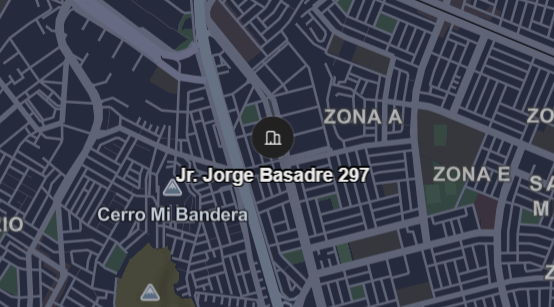
\includegraphics[width=0.55\textwidth]{ubicacion.png}
  \nota{Elaboración propia a partir de Google Maps (2026).}
\end{figure}

\section{Misión, Visión, Objetivo y Valores de la Empresa}

\subsection{Misión}
Diseñar, desarrollar e implementar soluciones informáticas confiables, seguras y adaptadas a las necesidades específicas de las municipalidades peruanas, contribuyendo a la modernización de su gestión administrativa y a la mejora continua de la atención al ciudadano, mediante un servicio técnico cercano y comprometido con cada entidad cliente.

\subsection{Visión}
Consolidarnos, para el año 2030, como la empresa referente a nivel nacional en la estandarización y modernización de los sistemas de gestión municipal, reconocida por la calidad, escalabilidad y sostenibilidad de sus soluciones tecnológicas, y por su aporte a la reducción de la brecha digital entre los gobiernos locales del Perú.

\subsection{Objetivo}
Normalizar progresivamente los sistemas informáticos utilizados por las municipalidades del Perú, reemplazando los desarrollos particularizados y dependientes de infraestructura física o de una sola persona por soluciones web estandarizadas, escalables y de fácil mantenimiento, que optimicen los procesos de gestión municipal y faciliten el acceso a la información para la toma de decisiones.

\subsection{Valores de la Empresa}

\begin{itemize}[leftmargin=1.25cm,itemsep=0pt,topsep=0pt]
  \item \textbf{Compromiso:} con la calidad del servicio brindado a cada municipalidad cliente y con el cumplimiento de los plazos y requerimientos acordados.
  \item \textbf{Confiabilidad:} garantizando la seguridad, disponibilidad e integridad de la información gestionada por los sistemas desarrollados.
  \item \textbf{Innovación:} incorporando de manera constante nuevas tecnologías (como la inteligencia artificial) que aporten valor a la gestión pública local.
  \item \textbf{Responsabilidad social:} entendiendo que las soluciones desarrolladas impactan directamente en la calidad del servicio que las municipalidades ofrecen a los ciudadanos.
  \item \textbf{Adaptabilidad:} ajustando las soluciones tecnológicas a la realidad, presupuesto y capacidad operativa de cada municipalidad atendida.
\end{itemize}

\section{Producto, Mercado y Cliente}

\subsection{Productos}
Consultoría Informática ofrece un sistema integral de gestión municipal orientado al área de rentas y trámites documentarios, que permite automatizar procesos como el registro de contribuyentes y propietarios, la administración del catastro urbano, el procesamiento de transferencias y bajas de propiedades, y la generación de reportes para la toma de decisiones. El producto se entrega actualmente como software de escritorio, aunque se encuentra en proceso de migración hacia una arquitectura web que permita un acceso más flexible y una mejor experiencia de uso para el personal municipal.

\subsection{Mercado}
El mercado objetivo de la empresa está conformado por el sector público local a nivel nacional, específicamente por las municipalidades distritales y provinciales del Perú que requieren digitalizar o modernizar su gestión administrativa. Dado que, según cifras del RENAMU, una parte significativa de los gobiernos locales del país aún no cuenta con sistemas digitales adecuados para sus procesos, este segmento representa un mercado con demanda potencial de crecimiento sostenido, especialmente en municipios distritales de mediana y pequeña escala.

\subsection{Clientes}
Los clientes de Consultoría Informática son las municipalidades peruanas, principalmente aquellas de escala distrital, que requieren soluciones tecnológicas adaptadas a sus procesos internos de gestión de rentas, catastro y trámites documentarios. Entre estos clientes se encuentra actualmente la Municipalidad de San Bartolo, entidad para la cual se desarrolla el presente proyecto de innovación.

\section{Estructura de la Organización}

La Figura~\ref{fig:organigrama} presenta la estructura de Consultoría Informática y, a la derecha, las áreas de la Municipalidad de San Bartolo que intervienen en el proyecto. Con borde rojo se resaltan las áreas y los cargos que usarán el sistema web, junto con el rol de acceso que tendrán en él (ADMIN, SUPERVISOR o CAJERO).

\begin{figure}[H]
\centering
\caption{Estructura de la organización y usuarios del sistema web}
\label{fig:organigrama}
\resizebox{\textwidth}{!}{%
\begin{tikzpicture}[
  font=\small,
  caja/.style={rectangle, draw, rounded corners=3pt, align=center, text width=3.3cm, minimum height=1.1cm, fill=white},
  usuario/.style={caja, draw=rojopim, very thick, fill=rojopim!6},
  grupo/.style={rectangle, draw=gray!60, dashed, rounded corners=6pt, inner sep=8pt},
  lin/.style={draw=gray!70, thick}
]
% --- Consultoría Informática ---
\node[caja, fill=gray!12] (ger) at (0,0) {\textbf{Gerente}\\Iván Casariego};
\node[caja] (dev1) at (-1.9,-2.0) {Practicante desarrollador\\Renzo A. Pérez G.};
\node[caja] (dev2) at (1.9,-2.0) {Practicante desarrollador\\Xavier E. Gerdez V.};
\draw[lin] (ger.south) -- ++(0,-0.45) -| (dev1.north);
\draw[lin] (ger.south) -- ++(0,-0.45) -| (dev2.north);
\node[grupo, fit=(ger)(dev1)(dev2), label={[font=\small\bfseries]above:Consultoría Informática (proveedor)}] (g1) {};
% --- Municipalidad de San Bartolo ---
\node[caja, fill=gray!12] (alc) at (11.1,0) {\textbf{Alcaldía}};
\node[usuario] (ren) at (8.9,-2.0) {Gerencia de Rentas\\(SUPERVISOR)};
\node[usuario] (sis) at (13.3,-2.0) {Administrador de sistemas\\(ADMIN)};
\node[usuario] (caj) at (7.0,-4.0) {Caja\\(CAJERO)};
\node[caja] (coa) at (10.8,-4.0) {Ejecutoría coactiva};
\draw[lin] (alc.south) -- ++(0,-0.45) -| (ren.north);
\draw[lin] (alc.south) -- ++(0,-0.45) -| (sis.north);
\draw[lin] (ren.south) -- ++(0,-0.45) -| (caj.north);
\draw[lin] (ren.south) -- ++(0,-0.45) -| (coa.north);
\node[grupo, fit=(alc)(ren)(sis)(caj)(coa), label={[font=\small\bfseries]above:Municipalidad de San Bartolo (cliente)}] (g2) {};
\draw[-{Stealth[length=2.5mm]}, thick, rojopim] (g1.east) -- node[above, font=\footnotesize, align=center]{desarrolla y\\mantiene} (g2.west|-g1.east);
\end{tikzpicture}}
\nota{Elaboración propia, con datos de la empresa y los roles definidos en el módulo de Accesibilidad del sistema. En rojo: usuarios del sistema web y su rol de acceso.}
\end{figure}

\section{Otra información relevante de la Empresa donde se desarrollará el Proyecto}

\subsection{Planificación y Gestión de la Entrevista}
En esta sección se describe la entrevista realizada con el encargado del área de Rentas de la Municipalidad de San Bartolo y con el responsable de la empresa, con el fin de identificar la problemática principal junto con sus causas y los beneficios que se obtendrán con la implementación del sistema web, a partir de una lista de preguntas.

\noindent\textbf{Fecha y hora:} \textbf{--- Encargado:}

\noindent\textbf{1. ¿Defina usted sus funciones en la empresa o en el área de Rentas?}

\noindent\textbf{2. ¿Por qué desea migrar el sistema actual (Sispredios) a un sistema web?}

\noindent\textbf{3. ¿Qué espera obtener a partir de la implementación del sistema web?}

\noindent\textbf{4. ¿Cuánto tiempo toma actualmente atender una incidencia o una corrección del sistema?}

\noindent\textbf{5. ¿Cómo se decide a qué contribuyentes se envían las cartas de aviso o los valores de cobranza?}

\subsection{Contexto del Proyecto: Municipalidad de San Bartolo}
El presente proyecto se desarrolla para la Municipalidad de San Bartolo, cliente de Consultoría Informática, que utiliza Sispredios para administrar el registro de contribuyentes y predios, la emisión de deudas del impuesto predial y los arbitrios, la caja y la cobranza ordinaria y coactiva. El sistema funciona instalado en los equipos de la municipalidad y depende de un servidor físico local, situación que se ha vuelto crítica con el proceso de reubicación del local municipal, ya que cualquier traslado del servidor interrumpe el acceso a la información.

En este contexto, la empresa decidió migrar Sispredios a una plataforma web estandarizada que pueda reutilizarse con otras municipalidades. La primera versión de la nueva base de datos agrupa la información en ocho dominios (administración, contribuyentes, catastro y predios, vehicular, parámetros tributarios, deuda y caja, cobranza y coactivo, y licencias) y, sobre el historial de deudas y pagos registrado durante años, incorpora un modelo de Machine Learning que estima el riesgo de morosidad de cada contribuyente. El avance de los módulos del nuevo sistema se presenta en el Anexo~\ref{anx:accesibilidad}.

% =====================================================================
% CAPÍTULO II: PLAN DE PROYECTO DE INNOVACIÓN / MEJORA / CREATIVIDAD
% =====================================================================
\chapter{Plan de Proyecto de Innovación / Mejora / Creatividad}

\section{Identificación del Problema Técnico en la Empresa}

\subsection{Problema Local de la Empresa}
\label{sec:problema-local}

Consultoría Informática desarrolla y vende software de gestión a municipalidades, y uno de sus productos es Sispredios, un sistema de gestión tributaria predial desarrollado en Visual FoxPro 9 como aplicación de escritorio. Se trata de un sistema de gran tamaño: el análisis de sus archivos muestra 219 formularios, 202 reportes y 252 tablas en su base de datos principal, que ocupa cerca de 3,5 GB, con alrededor de 1,9 millones de registros en su tabla de cuenta corriente y más de un millón de registros de pagos. % VERIFICAR el significado de la tabla de cuenta corriente al leer el código

Esta tecnología, además, ya no cuenta con respaldo del fabricante: Microsoft mantuvo el soporte extendido de Visual FoxPro hasta enero de 2015 \parencite{taft2007}. A esto se suma que el sistema funciona instalado en equipos locales, por lo que su uso queda limitado a la infraestructura física de cada entidad, y que cada municipalidad atendida cuenta con una solución distinta, construida de manera particular.

El problema principal identificado en la empresa es la \textit{falta de estandarización y sostenibilidad en el desarrollo y soporte de los sistemas de software entregados a las municipalidades}. Para priorizar sus causas se aplicó el método de Pareto (sección~\ref{sec:pareto}). Este problema se origina en las siguientes cuatro causas:

\causa{a}{Falta de estandarización en los sistemas desarrollados}\textcite{debortoli2017} describen que varias alcaldías del estado de Río Grande do Sul dependen de un sistema tributario heredado, desarrollado en COBOL, que no puede integrarse con aplicaciones web, y plantean migrarlo mediante una metodología común que alinee la tecnología con los procesos de todas ellas. En Consultoría Informática ocurre lo contrario: cada municipalidad atendida cuenta con una solución distinta, construida de manera particular, lo que dificulta el mantenimiento, la escalabilidad y la reutilización de código entre proyectos.

\causa{b}{Interfaces de usuario poco intuitivas, con un diseño UI/UX obsoleto e incómodo}\textcite{sommerville2011} explica que los sistemas heredados se basan en lenguajes y tecnologías que ya no se usan para desarrollar sistemas nuevos, y \textcite{bid2018} señalan que los procesos poco digitalizados hacen que un trámite ante una entidad pública de la región tome, en promedio, 5,4 horas. Sispredios presenta ese rasgo propio de las aplicaciones de escritorio antiguas: una interfaz formada por cientos de formularios sin un diseño común, que dificulta el uso cotidiano del personal municipal.

\causa{c}{Demoras en la atención de soporte técnico}La \textcite{gao2025} advierte que los sistemas heredados que dependen de \textit{software} sin soporte son los que más cuesta operar y mantener, y que absorben la mayor parte del gasto en tecnologías de la información. En la empresa, el conocimiento y la carga de trabajo se concentran en una sola persona y no existen procesos ni personal dedicado exclusivamente a las incidencias, situación que se agrava porque Visual FoxPro perdió el soporte del fabricante en 2015 \parencite{taft2007}.

\causa{d}{Limitación en el acceso a información estadística}\textcite{benedetto2026} señala que los métodos tradicionales de cobranza de las administraciones tributarias subnacionales son reactivos y dependen de procesos manuales. Lo mismo ocurre con Sispredios: no facilita la generación ni la consulta de reportes consolidados, y el historial de pagos y deudas acumulado durante años no se aprovecha para anticipar la morosidad ni para priorizar la cobranza, por lo que la gestión de cobro se vuelve reactiva. % VERIFICAR con el encargado de la empresa

Esta situación se refleja en la propia instalación de Sispredios. Algunos de sus programas auxiliares conservan rutas fijas a carpetas de otras municipalidades atendidas por la empresa, lo que muestra que el mismo código se copia y se adapta para cada cliente. Además, en la carpeta del sistema se conservan 35 versiones compiladas del ejecutable entre 2020 y 2025, siete de ellas generadas en solo tres días de mayo de 2023, porque cada corrección exige recompilar e instalar de nuevo todo el programa. Por último, para decidir a quién cobrar, el personal trabaja con listados exportados manualmente a hojas de cálculo, de los que se encontraron 20 archivos en la carpeta del sistema. Estos datos se detallan en el análisis cuantitativo del Capítulo~3.

\subsection{Problema Nacional}

En el artículo publicado en la \textit{Revista Amazónica de Ciencias Económicas}, \textcite{francoulco2026} analiza los datos del Registro Nacional de Municipalidades (RENAMU) de 2023 y describe que, de las 1,891 municipalidades del país, solo el 47,8\,\% cuenta con Mesa de Partes Virtual, mientras que el 52,2\,\% aún no implementa esta plataforma digital. El autor precisa que la brecha es mayor en el ámbito distrital: el 86,7\,\% de las municipalidades provinciales ya la implementó, frente a solo el 43,3\,\% de las distritales, grupo al que pertenece la Municipalidad de San Bartolo.

Esta brecha tecnológica se refleja en la gestión tributaria local. En el artículo publicado en la revista \textit{ECA Sinergia}, \textcite{romerocarazas2021} advierten una aparente pasividad fiscal en los gobiernos locales del Perú, que prefieren depender de las transferencias del gobierno central antes que desarrollar nuevas estrategias de recaudación del impuesto predial. En la misma línea, en el artículo publicado en \textit{Ciencia Latina Revista Científica Multidisciplinar}, \textcite{rojasbarbaran2021} revisan la gestión de la recaudación tributaria de las municipalidades del país y la presentan como un problema todavía no resuelto, del que dependen los ingresos propios con los que se financian los servicios locales.

El efecto de esta débil gestión se mide en la morosidad. En el artículo publicado en \textit{Ciencia Latina Revista Científica Multidisciplinar}, \textcite{riosvelasquez2022} reportan que en la Municipalidad Distrital de El Porvenir (Trujillo) la morosidad del impuesto predial fue de 72\,\% en 2019 y de 79\,\% en 2020, y que solo bajó a 65\,\% en 2021 cuando se aplicaron beneficios tributarios. Por su parte, en el artículo publicado en la revista \textit{ECA Sinergia}, \textcite{soriadiaz2022} describen una municipalidad donde los contribuyentes deben acudir en persona a realizar sus trámites porque la entidad no ofrece servicios en línea y su portal web está desactualizado, y señalan que la falta de datos actualizados de los contribuyentes limita el aumento de la recaudación.

Finalmente, en el artículo publicado en la revista \textit{Semestre Económico}, \textcite{cayatopa2026} analizan la recaudación predial del Perú entre 2012 y 2023 con un modelo de vectores autorregresivos con datos de panel, y encuentran que la pobreza tiene un efecto inverso sobre la recaudación, de $-0{,}21$ antes de la pandemia, que se intensificó a $-0{,}30$ durante y después de ella; por ello, proponen acciones focalizadas en los contribuyentes. En conjunto, estas investigaciones muestran que el problema identificado en Consultoría Informática no es un caso aislado: la desigual capacidad tecnológica de los gobiernos locales y la alta morosidad del impuesto predial son problemas nacionales, que requieren sistemas estandarizados y herramientas que indiquen a qué contribuyentes dirigir primero la cobranza.

\subsection{Problema Internacional}

En el libro publicado por el Banco Interamericano de Desarrollo, \textcite{bid2018} señalan que, en América Latina y el Caribe, un ciudadano necesita en promedio 5,4 horas para completar un trámite ante una entidad pública, que el 25\,\% de los trámites exige tres interacciones o más para resolverse y que el 29\,\% de los ciudadanos reportó haber pagado un soborno en el contexto de un servicio público en el último año. Los autores atribuyen esta situación a procesos poco digitalizados y no estandarizados, como los que todavía mantienen muchos gobiernos locales.

El rezago es mayor en el nivel local que en el nacional. En la Encuesta de Gobierno Electrónico 2024, \textcite{undesa2024} evaluó el portal de la ciudad más poblada de cada uno de los 193 Estados miembros: solo 151 contaban con un portal operativo, y de ellos 70 ciudades obtuvieron un nivel de servicios en línea inferior al de su propio país. El informe precisa que la provisión de servicios es el criterio con menor cumplimiento entre los seis evaluados, lo que confirma que los trámites municipales siguen siendo los menos digitalizados.

Este rezago afecta directamente al impuesto predial. En la revista \textit{Land Lines} del Lincoln Institute of Land Policy, \textcite{quintanilla2026} presentan la segunda edición del estudio \textit{Sistemas del impuesto predial en América Latina y el Caribe} e informan que la recaudación promedio de este impuesto en la región pasó de 0,35\,\% del producto interno bruto (PIB) en 2000 a solo 0,38\,\% en 2022, apenas un poco más de un tercio del promedio de los países de la OCDE, que supera el 1\,\%; además, ubican al Perú entre los países que recaudan menos del 0,3\,\% del PIB y estiman un potencial no aprovechado de entre 1\,\% y 1,25\,\% del PIB.

A ello se suma el costo de mantener sistemas heredados. En su informe al Congreso de los Estados Unidos, la \textcite{gao2025} indica que el gobierno federal destina cerca del 80\,\% de su gasto anual en tecnologías de la información, que supera los 100 mil millones de dólares, a operar y mantener sistemas existentes; de los 11 sistemas heredados que más requieren modernización, 8 usan lenguajes de programación obsoletos, 4 dependen de \textit{hardware} o \textit{software} sin soporte y 7 operan con vulnerabilidades de seguridad conocidas, situación comparable a la de Sispredios en Visual FoxPro.

El incumplimiento en el pago de tributos también es un problema mundial. En su informe comparativo sobre 58 administraciones tributarias, la \textcite{ocde2024} reporta que la deuda tributaria pendiente al cierre del año fiscal 2022 rondaba los 2,7 billones de euros, de los cuales cerca de 810 mil millones se consideraban cobrables. Frente a ello, las administraciones recurren a la analítica de datos: en el blog del Centro Interamericano de Administraciones Tributarias, \textcite{collosa2025} destacan, a partir del informe \textit{Tax Administration 2025} de la OCDE, que alrededor del 69\,\% de las administraciones evaluadas ya utiliza inteligencia artificial y otro 24\,\% se encuentra en fase de implementación.

En conjunto, estas fuentes confirman que el problema de fondo ---sistemas de gestión locales poco estandarizados, dependientes de tecnologías heredadas y con una cobranza que no aprovecha sus datos--- es una tendencia regional y mundial, lo que refuerza la pertinencia de un sistema web estandarizado con un componente de Machine Learning para priorizar la cobranza.

\subsection{Formulación del Problema}

\subtitulo{Problema General}

¿De qué manera la implementación de un sistema web de gestión tributaria predial, con un modelo de Machine Learning para estimar el riesgo de morosidad, mejorará la estandarización, el soporte y la sostenibilidad de los sistemas de software que Consultoría Informática brinda a las municipalidades?

\subtitulo{Problemas Específicos}

¿De qué manera la implementación de un sistema web con una arquitectura común y reutilizable (NestJS, React y PostgreSQL) mejorará la estandarización de los sistemas entregados a las municipalidades?

¿De qué manera el diseño de una interfaz web moderna, intuitiva y consistente (React y Tailwind CSS) mejorará la experiencia de uso del personal municipal frente a las interfaces obsoletas de escritorio?

¿De qué manera un sistema web con una única base de código, desplegada y actualizada de forma centralizada, reducirá las demoras en la atención de soporte técnico?

¿De qué manera un modelo de Machine Learning que estime el riesgo de morosidad de los contribuyentes mejorará el acceso a información estadística y la priorización de la cobranza en las municipalidades?

\section{Objetivo del Proyecto de Innovación}

\subsection{Objetivo General}

Implementar un sistema web de gestión tributaria predial, con un modelo de Machine Learning para estimar el riesgo de morosidad, que mejore la estandarización, el soporte y la sostenibilidad de los sistemas de software que Consultoría Informática brinda a las municipalidades.

\subsection{Objetivo Específico}

Desarrollar el sistema web sobre una arquitectura común y reutilizable (NestJS, React y PostgreSQL) para mejorar la estandarización de los sistemas entregados a las municipalidades.

Diseñar una interfaz web moderna, intuitiva y consistente (React y Tailwind CSS) para mejorar la experiencia de uso del personal municipal frente a las interfaces obsoletas de escritorio.

Centralizar el despliegue y la actualización del sistema en una única base de código para reducir las demoras en la atención de soporte técnico.

Entrenar e integrar un modelo de Machine Learning que estime el riesgo de morosidad de los contribuyentes para mejorar el acceso a información estadística y la priorización de la cobranza en las municipalidades.

\section{Antecedentes del Proyecto de Innovación / Mejora / Creatividad (Investigaciones Realizadas)}
\label{sec:antec}

Se revisaron quince investigaciones publicadas entre 2022 y 2026 (no mayores a cinco años): cinco antecedentes nacionales, cinco internacionales y cinco artículos científicos. De cada una se registran el problema, el objetivo, la metodología, los resultados estadísticos y la conclusión, para contrastarlos más adelante con los resultados del proyecto. Todas se relacionan con alguno de los dos ejes del proyecto: la gestión tributaria municipal apoyada en sistemas web, y la predicción de la morosidad o del incumplimiento tributario mediante técnicas de Machine Learning. En el Anexo~\ref{anx:antecedentes} se presenta un cuadro resumen.

\subsection{Antecedentes Nacionales}

En la tesis para optar el título de Ingeniero en Informática y Sistemas en la Universidad Nacional Agraria de la Selva, sustentada por \textcite{juncoaranciaga2023}, se presenta como título de investigación ``Evaluación comparativa en el desempeño de modelos de machine learning en la predicción de pagadores del impuesto predial de la ciudad de Tingo María para el año 2019''. El problema que aborda es la dificultad de la municipalidad para anticipar qué contribuyentes cumplirán con el pago del impuesto predial, lo que limita la planificación de la cobranza. Para ello, el autor aplicó una encuesta telefónica a 372 contribuyentes sobre factores socioeconómicos y de percepción, evaluó con la prueba Chi cuadrado la influencia de dichos factores en la clasificación de cada contribuyente como ``No pagador'', ``Impuntual'' o ``Pagador'', y entrenó modelos de árbol de decisión, máquinas de vectores de soporte (SVM), vecinos más cercanos (KNN), Naive Bayes, modelos de conjunto y redes neuronales, con validación cruzada de 10 pliegues y optimización de hiperparámetros. Como resultado, los modelos KNN y de redes neuronales obtuvieron las mayores exactitudes, de 97,04\,\% y 96,89\,\% respectivamente, y la prueba de Friedman mostró que las diferencias entre algoritmos eran estadísticamente significativas. Este antecedente es el más cercano al presente proyecto, pues demuestra en una municipalidad peruana que el aprendizaje automático puede clasificar a los contribuyentes según su comportamiento de pago del impuesto predial; a diferencia de dicho estudio, el presente proyecto propone utilizar el historial de deudas y pagos registrado en el propio sistema, en lugar de una encuesta.

En la tesis para optar el título profesional de Ingeniero de Sistemas e Informática en la Universidad Nacional de la Amazonía Peruana, sustentada por \textcite{pacaya2022}, se presenta como título de investigación ``Sistema informático web para la gestión de cobranza en el CETIC de la Municipalidad Distrital de Punchana, año 2021''. El estudio parte de la necesidad de mejorar la gestión de cobranza en dicha dependencia municipal. El objetivo fue desarrollar e implementar un sistema informático web que optimizara esa gestión. Los autores aplicaron un enfoque cuantitativo de nivel tecnológico aplicado, con diseño preexperimental, transversal y prospectivo, y midieron los tiempos de operación con cronómetro en 20 registros de pagos, 20 de matrículas, 10 de personal nuevo y 10 de generación de reportes. Como resultado, reportaron una efectividad de 126\,\% en el registro de pagos, 114\,\% en el registro de matrículas, 136\,\% en el registro de personal y 15,246\,\% en la generación de reportes de gestión, cifra muy superior a las demás, que los autores reportan tal como la obtuvieron. Se concluye que la implementación del sistema web optimiza la gestión de cobranza, por lo que se acepta la hipótesis de investigación. Este antecedente respalda la propuesta de reemplazar procesos de cobranza poco automatizados por un sistema web, y su forma de medir el efecto mediante tiempos de operación es aplicable al presente proyecto.

En la tesis de grado de la Universidad Nacional de la Amazonía Peruana, sustentada por \textcite{laulate2025}, se presenta como título de investigación ``Sistema web para la gestión de rentas de la Municipalidad Provincial de Maynas-2024''. El problema que aborda es la baja eficiencia operativa de la gestión de rentas municipales en tres procesos: la consulta de deudas, los pagos en línea y la entrega de notificaciones. El objetivo fue optimizar dicha eficiencia mediante un sistema web que además mejorara la experiencia de usuario. La metodología fue preexperimental con enfoque cuantitativo: se analizaron datos de 30 contribuyentes antes y después de implementar el sistema, con encuestas de usabilidad SUS y formularios de observación para medir los tiempos de proceso. Como resultados, el tiempo de consulta de deudas bajó de 16,47 a 2,50 minutos, el de pago de deudas de 18,43 a 2,50 minutos y el de entrega de notificaciones de 26,67 a 2,00 minutos, y el puntaje SUS promedio fue de 51,75, que indica una usabilidad moderada. Los autores concluyen que el sistema reduce los tiempos y estandariza los procesos, y recomiendan actualizarlo periódicamente, capacitar a los usuarios e incorporar recordatorios automáticos y más opciones de pago. Este antecedente muestra, en una municipalidad peruana, el efecto de un sistema web sobre la gestión de rentas, y su recomendación de incorporar recordatorios automáticos se vincula con la priorización de la cobranza que persigue el presente proyecto.

En la tesis para optar el título profesional de Contador Público en la Universidad Peruana Unión, sustentada por \textcite{campos2024}, se presenta como título de investigación ``La morosidad como predictor de la recaudación del impuesto predial de la Municipalidad Provincial de San Marcos -- Cajamarca''. La problemática es la baja recaudación del impuesto predial en dicha municipalidad, vinculada al pago tardío de los contribuyentes. El objetivo fue determinar la influencia de los factores de la morosidad en la recaudación del impuesto predial. Se aplicó un enfoque cuantitativo, con diseño descriptivo no experimental y una muestra no probabilística por conveniencia de 250 pobladores mayores de 18 años, a quienes se encuestó mediante formularios en línea; el análisis se realizó con el coeficiente alfa de Cronbach, la prueba de Kolmogorov-Smirnov y la correlación de Spearman en SPSS. Como resultados, la correlación global entre morosidad y recaudación fue de 0,578 (moderada y positiva), y por factores fue de 0,335 para el actitudinal, 0,401 para el social, 0,551 para el económico y 0,549 para el institucional. Se concluye que los factores actitudinales, sociales, económicos e institucionales contribuyen a la falta de pago. Este antecedente identifica factores que explican la morosidad predial, que el presente proyecto busca capturar de manera objetiva a partir del historial de pagos y no de encuestas.

En la tesis de Maestría en Gestión Pública presentada en la Universidad César Vallejo, sustentada por \textcite{paredes2022}, se presenta como título de investigación ``Cultura tributaria y su incidencia en la morosidad del impuesto predial en la Municipalidad Distrital de San Martín de Porres''. La problemática es la alta morosidad del impuesto predial en el distrito, de 44,63\,\% en 2019 y 55,12\,\% en 2020, lo que dificulta el cumplimiento de las metas de recaudación. El objetivo fue determinar cómo la cultura tributaria afecta la morosidad. La investigación fue básica, cuantitativa y correlacional-causal, con diseño no experimental y transversal; se encuestó a 100 contribuyentes mediante muestreo intencional y los datos se analizaron con regresión logística en SPSS. Como resultados, la cultura tributaria afecta significativamente la morosidad, con un R$^2$ de Nagelkerke de 0,22; la dimensión del sistema tributario fue significativa (10,9\,\%), al igual que el cumplimiento fiscal (6,5\,\%), mientras que la conciencia tributaria no lo fue. Se concluye que la cultura tributaria explica cerca del 22\,\% de la variación de la morosidad. Este antecedente sugiere que una parte importante de la morosidad no se explica solo por actitudes de los contribuyentes, por lo que otras fuentes de información, como su historial de pagos, pueden aportar a su estimación.

\subsection{Antecedentes Internacionales}

En la tesis de Maestría en Ingeniería -- Analítica de la Universidad Nacional de Colombia, sede Medellín, sustentada por \textcite{orozco2023}, se presenta como título de investigación ``Una propuesta de modelo para la determinación de la probabilidad de recaudo del impuesto vehicular en Antioquia''. El problema es que la administración tributaria departamental necesita priorizar sus procesos de fiscalización y aprovechar mejor los datos que ya registra. El objetivo fue desarrollar un modelo que estime la probabilidad de pago de cada contribuyente. El autor partió de una base de 15,160,030 registros de pagos del impuesto vehicular desde 1999, seleccionó el periodo 2015--2022 con 8,280,115 partidas y comparó Random Forest, regresión logística y Naive Bayes. Como resultado, Random Forest con partición aleatoria y sin la variable ``demora'' obtuvo un coeficiente de determinación $R^2$ de 0,408, un error cuadrático medio (MSE) de 0,066 y una raíz del error cuadrático medio (RMSE) de 0,257, los mejores valores entre los modelos comparados; al incluir la variable ``demora'' el $R^2$ subía a 0,987, pero el modelo dejaba de entregar probabilidades intermedias. Se concluye que Random Forest es el modelo más adecuado para ordenar a los contribuyentes según su probabilidad de pago. Este antecedente muestra que el historial de pagos de una administración subnacional basta para construir un modelo de priorización, como el que se plantea con el historial de Sispredios.

En la tesis de maestría de la Namibia University of Science and Technology, sustentada por \textcite{sifani2025}, se presenta como título de investigación ``Predictive Modelling of Taxpayer Compliance Behaviour Using Machine Learning at NamRA'' (Modelado predictivo del comportamiento de cumplimiento tributario mediante Machine Learning en la Namibia Revenue Agency). El problema es que la agencia necesita identificar con anticipación a los contribuyentes con probabilidad de incumplir. El objetivo fue explorar el uso del aprendizaje automático para predecir dicho comportamiento. Se ajustaron varios algoritmos de clasificación con validación cruzada de cinco pliegues, búsqueda en cuadrícula y búsqueda aleatoria de hiperparámetros en scikit-learn, y se usaron las técnicas SHAP y LIME para interpretar los resultados. Como resultado, la exactitud validada de los modelos estuvo entre 64\,\% y 68\,\%, y el mejor fue Random Forest optimizado con 68\,\%; los factores más influyentes fueron el grupo de ingreso, el periodo de la pandemia de COVID-19, la oficina de registro y el estado civil. Se concluye que el ajuste de hiperparámetros mejora el desempeño, aunque el autor reconoce que la exactitud es modesta. Este antecedente advierte que el modelo debe usarse como apoyo a la decisión y no como decisión automática, criterio que adopta el presente proyecto.

En la tesis de Maestría en Computación de la Escuela Politécnica Nacional del Ecuador, sustentada por \textcite{carrera2024}, se presenta como título de investigación ``Optimizing the collection process in credit risk management: A comparison of machine learning techniques for predicting payment probability at different stages of arrears'' (Optimización del proceso de cobranza: comparación de técnicas de Machine Learning para predecir la probabilidad de pago en distintas etapas de mora). El problema es que los modelos de regresión logística usados en la cobranza pierden precisión a medida que avanza la mora. El objetivo fue comparar XGBoost y redes neuronales artificiales con la regresión logística para generar puntajes de pago en cada etapa. Se trabajó con 125,459 registros de créditos y 86 variables predictoras, y el desempeño se midió con el estadístico de Kolmogorov-Smirnov (KS). Como resultado, en el modelo con todos los segmentos XGBoost alcanzó un KS de 74,05\,\% y la red neuronal 73,59\,\%, frente a 71,01\,\% de la regresión logística; en el segmento sin mora los valores fueron 63,36\,\%, 61,84\,\% y 56,42\,\%, respectivamente. Se concluye que los modelos de aprendizaje automático superan a la regresión logística en la mayoría de los segmentos. Este antecedente respalda comparar modelos de conjunto con una regresión logística de referencia para priorizar la cobranza.

En el trabajo de grado de la Especialización en Ciencia de Datos y Analítica de la Universidad Nacional Abierta y a Distancia de Colombia, sustentado por \textcite{lismoncaleano2026}, se presenta como título de investigación ``Segmentación de cartera y modelo predictivo de mora en propiedad horizontal mediante técnicas de machine learning''. El problema es que la cobranza de un conjunto residencial de 576 apartamentos en Bogotá se basaba solo en procedimientos operativos y reportes descriptivos. El objetivo fue segmentar la cartera y predecir el riesgo de mora para priorizar el recaudo. Bajo la metodología CRISP-DM, el autor segmentó la cartera con K-Means (coeficiente de silueta de 0,846 con $k=2$) y comparó regresión logística, Random Forest y XGBoost. Como resultado, Random Forest obtuvo un F1-score de 0,880 y un área bajo la curva ROC de 0,901, frente a 0,890 de XGBoost y 0,884 de la regresión logística, con una exactitud de 0,974 en el conjunto de prueba y un F1 promedio de 0,969 $\pm$ 0,038 en validación cruzada. Se concluye que la ciencia de datos permite priorizar acciones de recaudo basadas en evidencia. Este antecedente aplica a una cartera de deudas periódicas el mismo enfoque de segmentación y predicción que se propone para la cuenta corriente tributaria.

En la tesis de Maestría en Ciencia de Datos y Máquinas de Aprendizaje de la Universidad Internacional del Ecuador, sustentada por \textcite{encalada2025}, se presenta como título de investigación ``Diseño de una aplicación web para detección temprana de fraude de pagos en línea en el sector bancario, utilizando técnicas de aprendizaje automático explicable''. El problema es que el fraude en los pagos digitales genera pérdidas económicas y afecta la confianza de los usuarios. El objetivo fue desarrollar modelos predictivos e integrarlos en una aplicación web. Los autores aplicaron Scrum y Kanban, trabajaron con un conjunto de transacciones fuertemente desbalanceado (cerca de 99,9\,\% legítimas y 0,1\,\% fraudulentas) y compararon XGBoost, árbol de decisión, Random Forest y redes neuronales. Como resultado, XGBoost sin sobremuestreo alcanzó una exactitud de 0,9991 y un área bajo la curva ROC de 0,9677, con una precisión de 0,52 en la clase fraude, mientras que el árbol de decisión obtuvo un AUC de 0,8581. Se concluye que los modelos integrados en la aplicación web son una herramienta eficaz de apoyo al control. Este antecedente es cercano al presente proyecto porque integra el modelo predictivo dentro de una aplicación web y muestra que, con clases desbalanceadas, la exactitud por sí sola no basta para evaluar el modelo.

\subsection{Artículos Científicos}

En el artículo de investigación publicado en \textit{KSII Transactions on Internet and Information Systems} por \textcite{leekim2024}, titulado ``Deep Learning-based Delinquent Taxpayer Prediction: A Scientific Administrative Approach'', los autores señalan que la predicción de la morosidad tributaria ha sido poco explorada frente a la del riesgo crediticio. El objetivo fue predecir la morosidad de los impuestos locales de las personas en la República de Corea. Para ello combinaron información crediticia y tributaria de 354,130 contribuyentes (2015--2017), con unas 50 variables, y consideraron moroso a quien no pagaba dentro de los 30 días de recibida la notificación. Como resultado, el modelo de red neuronal convolucional (CNN) alcanzó una exactitud de 87,64\,\%, seguido de seq2seq con atención (84,43\,\%), ResNet (83,72\,\%), LSTM (83,39\,\%), Random Forest (82,86\,\%) y SVM (82,23\,\%), todos por encima de los modelos base de estudios previos (78,00\,\% y 78,86\,\%). Se concluye que una mejor predicción permite asignar los recursos administrativos con mayor eficiencia, objetivo que coincide con la priorización de la cobranza del presente proyecto.

En el artículo publicado en el \textit{IAES International Journal of Artificial Intelligence} por \textcite{ourdani2024}, titulado ``Towards a new approach to maximize tax collection using machine learning algorithms'', los autores señalan que la cobranza de la deuda tributaria local es un desafío para las autoridades de Marruecos, donde se registró un deterioro de 29\,\% en la recaudación. El objetivo fue segmentar a los contribuyentes según su riesgo de incumplimiento. Trabajaron con 2,739,934 registros de un tributo municipal entre 2010 y 2021, asignaron a cada deuda un puntaje según su ciclo de cobranza y compararon algoritmos de agrupamiento con los índices de silueta, Calinski-Harabasz y Davies-Bouldin. Como resultado, K-Means fue el más adecuado y clasificó a los contribuyentes en tres grupos: 8,557 ``malos'', 15,786 ``buenos'' y 41,796 ``excelentes''. Se concluye que identificar con exactitud a los deudores de alto riesgo permite aumentar la recaudación y reducir los recursos desperdiciados.

En el artículo publicado en \textit{METHOMIKA: Jurnal Manajemen Informatika \& Komputerisasi Akuntansi} por \textcite{sugiana2026}, titulado ``Prediksi kepatuhan wajib pajak PBB-P2 berbasis kecerdasan buatan dengan algoritma gradient boosting pada Badan Pendapatan Daerah Kabupaten Badung'' (Predicción del cumplimiento de los contribuyentes del impuesto predial PBB-P2 con inteligencia artificial y \textit{gradient boosting} en la Agencia de Ingresos de Badung, Indonesia), los autores señalan que el bajo cumplimiento del impuesto predial local hace que la recaudación no alcance sus metas y que la gestión tradicional es reactiva. El objetivo fue predecir qué contribuyentes cumplirán a partir de su historial de pagos. Se dividieron los datos en 70\,\% para entrenamiento y 30\,\% para prueba, se ajustaron los hiperparámetros de XGBoost con búsqueda en cuadrícula y se dio mayor peso a la clase minoritaria. Como resultado, el mejor modelo obtuvo un F1-macro de 0,7108 (con tasa de aprendizaje 0,2, profundidad 12 y 400 árboles), frente a 0,6657 de la configuración inicial, y las variables más influyentes fueron la ubicación del predio y el monto pagado. Se concluye que el modelo permite una gestión del impuesto predial más proactiva. Este artículo es el más cercano al presente proyecto, porque predice el pago del impuesto predial municipal con datos históricos de la propia administración.

En el artículo publicado en \textit{Electronic Government, an International Journal} por \textcite{omorog2022}, titulado ``Rethinking real property assessment and tax management system through an interoperable e-government framework'', los autores señalan que la recaudación del impuesto predial de los gobiernos locales de Filipinas es baja por valuaciones desactualizadas, procesos largos y la falta de una base de datos electrónica centralizada. El objetivo fue rediseñar el proceso mediante un sistema interoperable de valuación y gestión del impuesto predial (RPaTS) con tres módulos, evaluado con las métricas de calidad de la norma ISO 9126. Como resultado, el tiempo de procesamiento de una transacción bajó de 95 a 30 minutos y los usuarios calificaron el sistema con un promedio de 4,42 en escala de Likert. Se concluye que un sistema centralizado optimiza la gestión del impuesto predial. Este antecedente respalda la estandarización de la gestión tributaria municipal en un solo sistema y su forma de medir el efecto mediante tiempos de proceso.

En el artículo publicado en \textit{PLOS ONE} por \textcite{yang2025}, titulado ``Predictive modeling of tax compliance risks: A comparative study of machine learning approaches'', la autora señala que la gestión tributaria tradicional no logra identificar a tiempo el riesgo de incumplimiento. El objetivo fue construir modelos de predicción de riesgo tributario interpretables y comparar SVM, XGBoost y Random Forest. Se usaron 2,780 registros depurados de empresas de una administración tributaria regional de China (2021--2023), con una partición 70/30 y sobremuestreo SMOTE. Como resultado, Random Forest obtuvo una exactitud de 92,00\,\% y un F1 de 84,26\,\% en el sector manufacturero, y una exactitud de 93,39\,\% y un F1 de 88,54\,\% en el de servicios, frente a 86,82\,\% de XGBoost y 85,18\,\% de SVM en manufactura. Se concluye que Random Forest ofrece la mejor exactitud y estabilidad, aunque los resultados se limitan a una jurisdicción. Este antecedente respalda la elección de Random Forest como uno de los modelos candidatos del presente proyecto.

\section{Justificación del Proyecto de Innovación / Mejora / Creatividad}

El proyecto se justifica desde cinco perspectivas, cada una vinculada directamente con el problema principal, sus causas y la solución propuesta. La Tabla~\ref{tab:tipos_just} resume la relación de cada justificación con el proyecto, y a continuación se desarrolla cada una.

\begin{table}[H]
\centering
\caption{Justificaciones del proyecto y su relación con el problema}
\label{tab:tipos_just}
\singlespacing\small
\begin{tabular}{@{}L{2.6cm}L{9.6cm}L{2.0cm}@{}}
\toprule
\textbf{Justificación} & \textbf{Relación con el proyecto} & \textbf{Causas} \\
\midrule
Práctica & Resuelve un problema real y vigente de la empresa y de la municipalidad: el mantenimiento de Sispredios y la cobranza sin priorizar. & a), c), d) \\
Tecnológica & El problema nace de una tecnología sin soporte (Visual FoxPro 9) y la solución es una nueva arquitectura web con Machine Learning. & a), b), c) \\
Económica & Las cuatro causas generan pérdidas que se cuantifican en la sección~\ref{sec:perdidas} y que la mejora reduce. & a), b), c), d) \\
Social & El sistema lo usan funcionarios municipales y sus resultados llegan a los vecinos que pagan sus tributos. & b), d) \\
Legal & El sistema automatiza procesos regulados por normas tributarias y trata datos personales de los contribuyentes. & d) \\
\bottomrule
\end{tabular}
\nota{Elaboración propia, a partir de las causas identificadas en la sección~\ref{sec:problema-local}.}
\end{table}

\subsection{Justificación Práctica}

El proyecto se justifica en la práctica porque responde a una necesidad concreta y actual: Consultoría Informática debe mantener un sistema de escritorio distinto por cada municipalidad, cada corrección exige recompilar e instalar todo el programa, y la Municipalidad de San Bartolo decide a quién cobrar con listados armados a mano. El sistema web reemplaza ese proceso por una sola aplicación, actualizada de forma centralizada, que el personal de Rentas, Caja y Cobranza usa desde el navegador, y entrega un puntaje de riesgo que indica qué deudas atender primero. El avance del sistema (Anexo~\ref{anx:accesibilidad}) muestra que la solución ya se está construyendo sobre los procesos reales del área de Rentas.

\subsection{Justificación Tecnológica}

Sispredios fue desarrollado en Visual FoxPro 9, una tecnología cuyo soporte extendido terminó en enero de 2015 \parencite{taft2007}, y funciona como aplicación de escritorio instalada en equipos locales y dependiente de un servidor físico. El proyecto se justifica porque reemplaza esa base por una arquitectura web con tecnologías vigentes y de uso extendido: NestJS y TypeScript en el servidor, React y Tailwind CSS en la interfaz, y PostgreSQL con Prisma como base de datos. Esta arquitectura permite acceder al sistema desde cualquier lugar con conexión a internet, desplegar y actualizar una única versión de forma centralizada, y reutilizar el mismo producto en otras municipalidades en lugar de mantener una copia distinta por cliente. Además, incorpora desde su inicio un control de acceso basado en roles y niveles, con autenticación mediante tokens JWT, y un componente de Machine Learning que aprovechará el historial de deudas y pagos acumulado durante años.

\subsection{Justificación Económica}
\label{sec:just-econ}

El proyecto se justifica económicamente porque las cuatro causas del problema generan pérdidas que hoy asumen la empresa y la municipalidad: horas de desarrollo duplicadas al adaptar cada corrección a varias copias del sistema, horas de atención perdidas con una interfaz lenta, horas detenidas en cada nueva versión del ejecutable y gastos de cobranza que no se recuperan. Con los parámetros de la sección~\ref{sec:perdidas}, estas pérdidas se estiman en \soles{\PerdMes} al mes, es decir, \soles{\PerdAnio} al año. Con una única base de código, cada corrección se despliega una sola vez para todas las municipalidades, la atención en ventanilla se acelera y la cobranza se dirige primero a las deudas con mayor riesgo; los antecedentes muestran reducciones de tiempo de 16,47 a 2,50 minutos por consulta de deuda \parencite{laulate2025} y de 95 a 30 minutos por transacción predial \parencite{omorog2022}.

\subsection{Justificación Social}

El proyecto beneficia, en primer lugar, al personal de las áreas de Rentas, Caja y Cobranza de la Municipalidad de San Bartolo, que podrá acceder al sistema desde cualquier lugar con conexión a internet, sin depender de un servidor físico ni de los equipos donde se instaló la aplicación de escritorio, y con una interfaz web más clara que reduce la curva de aprendizaje. En segundo lugar, beneficia a los vecinos del distrito, porque una atención más ágil en ventanilla y una cobranza ordenada se traducen en un mejor servicio y en información más confiable sobre sus deudas. Además, el modelo de riesgo de morosidad permite que la municipalidad oriente primero sus recordatorios y facilidades de pago hacia los contribuyentes con mayor probabilidad de atrasarse, antes de que su deuda pase a cobranza coactiva, etapa en la que se generan costas, embargos y mayor carga para el vecino. Finalmente, al mejorar la recaudación del impuesto predial, la municipalidad dispone de más recursos para financiar los servicios públicos locales que recibe la comunidad.

\subsection{Justificación Legal}

El proyecto se sustenta en el Decreto Legislativo N.\textsuperscript{o}~1412, Ley de Gobierno Digital \parencite{dleg1412}, que establece el marco para el uso de las tecnologías digitales en las entidades de la administración pública, entre ellas los gobiernos locales, con el fin de mejorar la prestación de servicios a los ciudadanos. Asimismo, la Ley N.\textsuperscript{o}~31814 \parencite{ley31814} promueve el uso de la inteligencia artificial en favor del desarrollo económico y social del país, en un entorno seguro, ético y responsable, lo que respalda la incorporación del modelo de Machine Learning dentro del sistema.

En cuanto al dominio tributario, el sistema automatiza procesos regulados por el Texto Único Ordenado de la Ley de Tributación Municipal \parencite{tuoltm}, que define el impuesto predial y su forma de cálculo, y por el Texto Único Ordenado del Código Tributario \parencite{codigotributario}, que regula, entre otros aspectos, los intereses moratorios y el procedimiento de cobranza. La cobranza coactiva se rige por la Ley de Procedimiento de Ejecución Coactiva \parencite{ley26979}. Por último, el tratamiento de los datos de los contribuyentes se rige por la Ley N.\textsuperscript{o}~29733, Ley de Protección de Datos Personales \parencite{ley29733}; por ello, el modelo de Machine Learning trabaja solo con el código interno del contribuyente, sin utilizar nombres ni documentos de identidad, y su resultado es solo un apoyo para que el personal priorice la cobranza, no una decisión automática.

\section{Marco Teórico y Conceptual}
\label{sec:marco}

\subsection{Fundamentos teóricos del Proyecto de Innovación}

Las variables del estudio se identifican a partir del título del proyecto y se alinean con el problema principal y sus causas. La \textbf{Variable 1} es el \textit{sistema web de gestión tributaria predial}, que atiende las causas a), b) y c): la falta de estandarización, la interfaz obsoleta y las demoras en el soporte. La \textbf{Variable 2} es la \textit{estimación del riesgo de morosidad con Machine Learning}, que atiende la causa d): el acceso limitado a información estadística para priorizar la cobranza. Cada variable se desarrolla en temas (A, B, C\ldots) y subtemas (A.1, A.2\ldots), y cada uno cierra con su relación con el sistema; la Tabla~\ref{tab:jerarquia} del Anexo~\ref{anx:jerarquia} resume esta jerarquía.

\subsubsection{Variable 1: Sistema web de gestión tributaria predial}

Un sistema web de gestión tributaria predial es un sistema informático al que el personal municipal accede desde el navegador para registrar a los contribuyentes y sus predios, calcular y emitir la deuda, cobrarla y hacer su seguimiento. Para comprenderlo, se desarrolla en cuatro temas: el sistema informático, la aplicación web, la migración de sistemas heredados y la gestión tributaria predial que el sistema automatiza.

\noindent\textbf{\textit{A) Sistema informático.}} \textcite{raya2014} definen un sistema informático como un conjunto de partes interrelacionadas que emplea un ordenador con dispositivos programables para capturar, almacenar y procesar datos (p.~18). Los autores precisan que, aunque su estructura puede dividirse en partes, funcionalmente es indivisible, ya que un sistema informático al que le falta alguno de sus componentes deja de funcionar; dichos componentes son el físico, el lógico y el humano (p.~18).

\noindent\textbf{\textit{A.1) Componente físico (hardware).}} Es el conjunto de equipos sobre los que se ejecuta el sistema \parencite{raya2014}. \textit{Relación con el sistema:} corresponde al servidor donde se despliega la aplicación y a los equipos de los funcionarios, que solo necesitan un navegador; esto elimina la dependencia del servidor físico instalado en la municipalidad.

\noindent\textbf{\textit{A.2) Componente lógico (software).}} Comprende el software de base, que permite el funcionamiento del equipo, y el software de aplicación, que resuelve las tareas del usuario \parencite{raya2014}. \textit{Relación con el sistema:} el software de base es el entorno Node.js y el gestor PostgreSQL; el software de aplicación es el sistema web de rentas, formado por el servidor (NestJS) y la interfaz (React).

\noindent\textbf{\textit{A.3) Componente humano.}} Son las personas que operan y mantienen el sistema \parencite{raya2014}. \textit{Relación con el sistema:} corresponde al personal de Rentas, Caja y Cobranza de la municipalidad, resaltado en rojo en la Figura~\ref{fig:organigrama}, y al equipo de desarrollo de la empresa.

\noindent\textbf{\textit{B) Aplicación web y arquitectura cliente-servidor.}} Una aplicación web es un sistema al que se accede mediante un navegador a través de internet, sin instalarlo en cada equipo. \textcite{fielding2000} describe el estilo arquitectónico REST (\textit{Representational State Transfer}) para sistemas distribuidos, basado en la separación entre cliente y servidor, la comunicación sin estado, el uso de caché, una interfaz uniforme y una organización en capas. \textit{Relación con el sistema:} el sistema se construye con esta arquitectura, lo que permite cambiar la interfaz sin tocar la lógica de negocio y reutilizar el mismo servidor en distintas municipalidades, atacando la causa a).

\noindent\textbf{\textit{B.1) Interfaz de programación (API REST).}} Siguiendo las restricciones de \textcite{fielding2000}, cada operación se expone como un recurso al que el cliente accede con solicitudes independientes entre sí. \textit{Relación con el sistema:} el servidor NestJS expone servicios como \texttt{/users}, \texttt{/roles} o \texttt{/niveles}, que consume la interfaz en React (Anexo~\ref{anx:accesibilidad}).

\noindent\textbf{\textit{B.2) Base de datos relacional.}} \textcite{codd1970} propone el modelo relacional, en el que los datos se organizan en relaciones (tablas) independientes de su forma de almacenamiento físico, lo que permite consultarlos y mantener su consistencia sin depender de cada programa. \textit{Relación con el sistema:} la base de datos PostgreSQL reemplaza las 252 tablas DBF de Sispredios, con llaves foráneas que garantizan que cada pago esté ligado a su deuda.

\noindent\textbf{\textit{B.3) Seguridad y control de acceso.}} \textcite{sandhu1996} presentan el control de acceso basado en roles (RBAC), en el que los permisos se asocian a roles y los usuarios se asignan a los roles que les corresponden. A su vez, el JSON Web Token es, según \textcite{rfc7519}, un medio compacto y firmado de transferir información entre dos partes. \textit{Relación con el sistema:} el módulo de Accesibilidad aplica RBAC (usuarios, roles, niveles y accesos por rol) y entrega al ingresar un token JWT que lleva los niveles del usuario; las contraseñas se guardan cifradas con bcrypt.

\noindent\textbf{\textit{C) Sistemas heredados y su migración.}} \textcite{sommerville2011} define los sistemas heredados (\textit{legacy}) como sistemas antiguos que siguen siendo esenciales para la organización, pero que se basan en lenguajes y tecnologías que ya no se usan para desarrollar sistemas nuevos, por lo que su mantenimiento es cada vez más costoso y riesgoso. El autor plantea que la organización debe evaluarlos y decidir entre desecharlos, seguir manteniéndolos, transformarlos mediante reingeniería o reemplazarlos por un sistema nuevo. \textit{Relación con el sistema:} Sispredios es un sistema heredado en Visual FoxPro 9; el proyecto opta por reemplazarlo por un sistema web, usando su base de datos solo como referencia histórica, lo que ataca las causas b) y c).

\noindent\textbf{\textit{D) Gestión tributaria predial.}} Es el conjunto de procesos con los que la municipalidad determina, cobra y controla el impuesto predial y los arbitrios. Se desarrolla en tres subtemas que corresponden a los módulos del sistema.

\noindent\textbf{\textit{D.1) Impuesto predial.}} De acuerdo con el artículo 8 del Texto Único Ordenado de la Ley de Tributación Municipal, el impuesto predial es de periodicidad anual, grava el valor de los predios urbanos y rústicos, y su recaudación, administración y fiscalización corresponden a la municipalidad distrital donde se ubica el predio \parencite{tuoltm}. \textit{Relación con el sistema:} el módulo de Rentas registra los predios y sus declaraciones juradas, calcula el impuesto y genera la deuda en la cuenta corriente por tributo, año y cuota.

\noindent\textbf{\textit{D.2) Cobranza ordinaria.}} Cuando la deuda no se paga a tiempo, la administración emite valores como la orden de pago o la resolución de determinación, regulados por el Código Tributario \parencite{codigotributario}. \textit{Relación con el sistema:} el sistema registra las cartas de aviso, los valores y los convenios de fraccionamiento, y la caja registra cada pago con su recibo.

\noindent\textbf{\textit{D.3) Cobranza coactiva.}} Si la deuda persiste, el valor se deriva al ejecutor coactivo, que inicia el procedimiento regulado por la Ley de Procedimiento de Ejecución Coactiva \parencite{ley26979}. \textit{Relación con el sistema:} el módulo de Coactiva recibe los valores transferidos por Rentas y los asigna para su seguimiento.

\subsubsection{Variable 2: Estimación del riesgo de morosidad con Machine Learning}

La estimación del riesgo de morosidad consiste en calcular, para cada contribuyente y cada año, la probabilidad de que su comportamiento de pago corresponda a uno de tres grupos ---Puntual, Tardío o Incobrable---, a partir del historial de deudas y pagos registrado en el sistema. Se desarrolla en cinco temas: la morosidad tributaria, el Machine Learning, los algoritmos de clasificación, la evaluación de los modelos y la priorización de la cobranza. Cada tema presenta, además de su definición, la forma matemática con la que se aplica en el modelo.

\noindent\textbf{\textit{A) Morosidad tributaria.}} La morosidad se presenta cuando el contribuyente no paga su deuda dentro del plazo establecido; según el artículo 33 del Código Tributario, el tributo no pagado a tiempo devenga un interés moratorio \parencite{codigotributario}. Su magnitud puede ser alta: \textcite{paredes2022} reporta una morosidad predial de 44,63\,\% en 2019 y 55,12\,\% en 2020 en San Martín de Porres, y \textcite{riosvelasquez2022}, de 79\,\% en 2020 en El Porvenir. Sin embargo, no todo moroso es igual: quien paga con unos meses de atraso requiere un recordatorio, mientras que quien no paga en todo el año requiere una gestión intensiva. Por ello, el proyecto clasifica a cada contribuyente $i$ en el año $T$ según el atraso $d_{ij}$, en días, de cada una de sus cuotas $j$ de impuesto predial y arbitrios:
\begin{equation}
y_{iT}=\begin{cases}
\text{Puntual} & \text{si } d_{ij}\le 90 \text{ para todas sus cuotas } j,\\
\text{Incobrable} & \text{si alguna cuota } j \text{ sigue impaga al cumplir } 365 \text{ días de su vencimiento},\\
\text{Tardío} & \text{en los demás casos.}
\end{cases}
\label{eq:grupos}
\end{equation}
\textit{Relación con el sistema:} el sistema calcula la mora de cada cuota; el grupo $y_{iT}$ de la Ecuación~\eqref{eq:grupos} es la variable que el modelo busca anticipar al inicio de cada año.

\noindent\textbf{\textit{B) Machine Learning.}} \textcite{mitchell1997} define el aprendizaje automático así: ``se dice que un programa de computadora aprende de la experiencia E con respecto a una clase de tareas T y una medida de desempeño P, si su desempeño en las tareas de T, medido por P, mejora con la experiencia E'' (p.~2). \textit{Relación con el sistema:} la tarea T es estimar el grupo de pago de cada contribuyente; la experiencia E es el historial de deudas y pagos de Sispredios; y la medida P son las métricas del tema D).

\noindent\textbf{\textit{B.1) Aprendizaje supervisado y clasificación.}} En el aprendizaje supervisado el algoritmo aprende de ejemplos cuyo resultado ya se conoce; cuando ese resultado es una categoría, el problema es de clasificación \parencite{mitchell1997}. Formalmente, se dispone de $N$ ejemplos $\{(\mathbf{x}_i, y_i)\}_{i=1}^{N}$, donde $\mathbf{x}_i$ es el vector de variables del contribuyente y $y_i$ su grupo, y se busca una función que estime la probabilidad de cada grupo $k$:
\begin{equation}
\hat{p}_{ik}=\hat{P}(y_i=k\mid\mathbf{x}_i),\qquad k\in\{\text{Puntual},\ \text{Tardío},\ \text{Incobrable}\},\qquad \sum_{k}\hat{p}_{ik}=1.
\label{eq:proba}
\end{equation}
\textit{Relación con el sistema:} cada contribuyente-año histórico, con las variables calculadas al 1 de enero y el grupo que tuvo al cierre, es un ejemplo de entrenamiento.

\noindent\textbf{\textit{B.2) Proceso CRISP-DM.}} \textcite{chapman2000} proponen un proceso estándar de minería de datos en seis fases: comprensión del negocio, comprensión de los datos, preparación de los datos, modelado, evaluación y despliegue. \textit{Relación con el sistema:} el modelo de riesgo siguió estas fases (sección~\ref{sec:crisp}), y su resultado se despliega dentro del propio sistema web, como en \textcite{encalada2025}.

\noindent\textbf{\textit{C) Algoritmos de clasificación.}} Son los métodos con los que el modelo aprende a separar a los contribuyentes según su grupo de pago. Se compararon tres algoritmos.

\noindent\textbf{\textit{C.1) Regresión logística multinomial.}} \textcite{hosmer2013} describen la regresión logística como el modelo estándar para relacionar un resultado categórico con un conjunto de variables explicativas, mediante la probabilidad de que ocurra cada categoría. Con $K$ grupos, la probabilidad se obtiene con la función \textit{softmax}:
\begin{equation}
P(y=k\mid\mathbf{x})=\frac{e^{\beta_{0k}+\boldsymbol{\beta}_{k}^{\top}\mathbf{x}}}{\sum_{m=1}^{K}e^{\beta_{0m}+\boldsymbol{\beta}_{m}^{\top}\mathbf{x}}},
\label{eq:softmax}
\end{equation}
donde $\beta_{0k}$ y $\boldsymbol{\beta}_{k}$ son los coeficientes del grupo $k$, estimados por máxima verosimilitud. Con dos grupos, la Ecuación~\eqref{eq:softmax} se reduce a la función logística $P(y=1\mid\mathbf{x})=1/\bigl(1+e^{-(\beta_0+\boldsymbol{\beta}^{\top}\mathbf{x})}\bigr)$. \textit{Relación con el sistema:} es el modelo de referencia, por ser fácil de interpretar por el personal de Rentas.

\noindent\textbf{\textit{C.2) Random Forest.}} \textcite{breiman2001} lo define como una combinación de árboles de decisión, cada uno construido con un vector aleatorio muestreado de forma independiente, cuya predicción resulta del conjunto. Cada árbol divide los datos eligiendo, en cada nodo, la variable que más reduce la impureza de Gini, y el bosque promedia las probabilidades de sus $B$ árboles:
\begin{equation}
G=1-\sum_{k=1}^{K}p_{k}^{2},\qquad\qquad \hat{P}(y=k\mid\mathbf{x})=\frac{1}{B}\sum_{b=1}^{B}\hat{P}_{b}(y=k\mid\mathbf{x}),
\label{eq:rf}
\end{equation}
donde $p_k$ es la proporción de ejemplos del grupo $k$ en el nodo y $\hat{P}_{b}$ es la probabilidad que estima el árbol $b$. \textit{Relación con el sistema:} varios antecedentes obtuvieron con él su mejor desempeño \parencite{orozco2023,sifani2025,lismoncaleano2026,yang2025}; en el proyecto se usan $B=400$ árboles y fue el modelo elegido.

\noindent\textbf{\textit{C.3) Gradient boosting.}} \textcite{friedman2001} propone construir un modelo aditivo por etapas, añadiendo en cada paso un nuevo árbol $h_m$ que corrige los errores del modelo anterior:
\begin{equation}
F_{m}(\mathbf{x})=F_{m-1}(\mathbf{x})+\nu\,h_{m}(\mathbf{x}),
\label{eq:gb}
\end{equation}
donde $h_m$ se ajusta al gradiente negativo de la función de pérdida y $\nu$ es la tasa de aprendizaje; XGBoost es una de sus implementaciones. \textit{Relación con el sistema:} se comparó con Random Forest, pues obtuvo buenos resultados en el impuesto predial \parencite{sugiana2026} y en la cobranza \parencite{carrera2024}.

\noindent\textbf{\textit{D) Evaluación de modelos de clasificación.}} \textcite{fawcett2006} explica que la matriz de confusión registra los aciertos y errores del clasificador, de la que se obtienen la precisión y la sensibilidad (\textit{recall}), y que las gráficas ROC permiten comparar clasificadores; el área bajo la curva (AUC) resume en un solo valor su capacidad para distinguir entre las clases. Para cada grupo $k$, con sus verdaderos positivos ($VP_k$), falsos positivos ($FP_k$) y falsos negativos ($FN_k$):
\begin{equation}
\text{Precisión}_k=\frac{VP_k}{VP_k+FP_k},\qquad
\text{Recall}_k=\frac{VP_k}{VP_k+FN_k},\qquad
F1_k=\frac{2\cdot\text{Precisión}_k\cdot\text{Recall}_k}{\text{Precisión}_k+\text{Recall}_k}.
\label{eq:metricas}
\end{equation}
El F1 macro es el promedio simple de $F1_k$ en los tres grupos, de modo que cada grupo pesa lo mismo aunque tenga menos casos. Como el modelo entrega probabilidades que luego se multiplican por la deuda, también se mide su calidad con la pérdida logarítmica (\textit{log-loss}), que equivale a la verosimilitud negativa con la que se estima la regresión logística \parencite{hosmer2013}:
\begin{equation}
\text{Log-loss}=-\frac{1}{N}\sum_{i=1}^{N}\sum_{k=1}^{K}\mathbf{1}[y_i=k]\,\log\hat{p}_{ik},
\label{eq:logloss}
\end{equation}
donde $\mathbf{1}[y_i=k]$ vale 1 si el contribuyente $i$ pertenece al grupo $k$ y 0 en otro caso; cuanto menor es el valor, más fieles son las probabilidades. \textit{Relación con el sistema:} el modelo se eligió por el menor log-loss y se reporta con el F1 macro, la sensibilidad del grupo Incobrable y el AUC de cada grupo frente a los demás, porque la exactitud por sí sola puede engañar cuando los grupos están desbalanceados \parencite{encalada2025}.

\noindent\textbf{\textit{E) Priorización de la cobranza según el riesgo.}} Las administraciones tributarias cuentan con personal y tiempo limitados; una mejor predicción de la morosidad les permite asignar sus recursos de forma más eficiente \parencite{leekim2024} e identificar a los deudores de alto riesgo para aumentar la recaudación \parencite{ourdani2024}. En el proyecto, cada contribuyente recibe una deuda esperada no recuperada ($DE_i$), que combina su riesgo con el monto en juego, y la lista de cobranza se ordena de mayor a menor $DE_i$. La eficacia de la lista se mide con la cobertura: qué parte de la deuda que realmente no se recuperó ($NR_i$) se concentra en el primer $n$\,\% de la lista:
\begin{equation}
DE_i=\hat{p}_{i,\text{Incobrable}}\times D_i\times\phi,\qquad\qquad
\text{Cobertura}(n)=\frac{\sum_{i\,\in\,\text{primer } n\text{\,\%}}NR_i}{\sum_{i}NR_i},
\label{eq:priorizacion}
\end{equation}
donde $D_i$ es la deuda emitida del año y $\phi$ es la fracción de su deuda anual que, en promedio, deja sin pagar un contribuyente incobrable (0,382, medida en los años de entrenamiento). \textit{Relación con el sistema:} la lista ordenada se muestra al personal de Rentas, con el grupo y la acción sugerida, como apoyo para ordenar el envío de cartas y valores, sin reemplazar su decisión.

\subsection{Conceptos y términos utilizados}

Los siguientes términos se utilizan a lo largo del documento y corresponden al dominio de la gestión tributaria municipal, a la seguridad del sistema y a la documentación de la base de datos del sistema desarrollado.

\begin{itemize}[leftmargin=1.25cm,itemsep=0pt,topsep=0pt]
  \item \textbf{Predio:} inmueble formado por el terreno y lo construido sobre él; puede ser una casa, un local, un terreno vacío o una cochera.
  \item \textbf{Autovalúo:} valor oficial del predio en soles, calculado cada año con los aranceles y las características de la construcción. Es la base del impuesto predial.
  \item \textbf{Arbitrios municipales:} tasas que pagan los vecinos por los servicios de limpieza pública (barrido y recojo de residuos), parques y jardines, y serenazgo.
  \item \textbf{UIT (Unidad Impositiva Tributaria):} monto de referencia fijado cada año por el Estado; los tramos del impuesto predial y muchas multas se expresan en UIT.
  \item \textbf{Cuenta corriente tributaria:} estado de cuenta de cada contribuyente, formado por la lista de sus deudas por tributo, año y cuota.
  \item \textbf{Declaración jurada:} documento en el que el contribuyente declara su predio y sus construcciones, y a partir del cual se calcula su impuesto.
  \item \textbf{Orden de Pago (OP):} documento con el que la municipalidad exige una deuda ya declarada pero no pagada.
  \item \textbf{Resolución de Determinación (RD):} documento con el que la municipalidad fija la deuda cuando el contribuyente no la declaró.
  \item \textbf{Cobranza coactiva:} etapa final del cobro forzoso, en la que, mediante un expediente a cargo del ejecutor coactivo, se pueden embargar cuentas o bienes del deudor.
  \item \textbf{Fraccionamiento o convenio:} acuerdo para pagar una deuda en cuotas en lugar de hacerlo al contado.
  \item \textbf{Mora y reajuste:} la mora es el interés por pagar tarde; el reajuste es la actualización de la deuda por inflación.
  \item \textbf{Extorno:} anulación de un pago mal registrado; no se borra, sino que cambia de estado para dejar rastro.
  \item \textbf{Catastro:} inventario técnico de todos los predios del distrito, con su ubicación, medidas y características.
  \item \textbf{Sistema heredado (legado):} sistema informático antiguo que sigue en uso, en este caso Sispredios, desarrollado en Visual FoxPro 9.
  \item \textbf{Aplicación web:} sistema al que se accede mediante un navegador a través de internet, sin necesidad de instalarlo en cada equipo.
  \item \textbf{API REST:} interfaz con la que la aplicación de usuario solicita datos y operaciones al servidor mediante solicitudes independientes entre sí.
  \item \textbf{Rol:} perfil de usuario del sistema (por ejemplo, administrador o cajero) que reúne los niveles de acceso que le corresponden.
  \item \textbf{Nivel:} permiso sobre una pantalla (módulo) o una función (subnivel) del sistema, identificado con un código estable.
  \item \textbf{Token JWT:} credencial firmada que el sistema entrega al iniciar sesión y que incluye los niveles del usuario.
  \item \textbf{Riesgo de morosidad:} probabilidad, estimada por el modelo de Machine Learning, de que un contribuyente pertenezca en el año a cada grupo de pago: Puntual (paga con 90 días de atraso como máximo), Tardío (paga después, pero antes de un año) o Incobrable (alguna cuota sigue impaga al año de vencer).
  \item \textbf{Deuda esperada no recuperada:} monto en soles que se espera que un contribuyente deje sin pagar en el año; ordena la lista de cobranza.
\end{itemize}

% =====================================================================
% CAPÍTULO III: ANÁLISIS DE LA SITUACIÓN ACTUAL
% =====================================================================
\chapter{Análisis de la Situación Actual}

\section{Diagrama del proceso, mapa de flujo de valor y/o diagrama de operación actual}

\subsection{Proceso actual de la empresa -- sin la intervención del Software}

El proceso de gestión tributaria predial que hoy atiende Sispredios en la Municipalidad de San Bartolo se modeló en notación BPMN 2.0 (Figura~\ref{fig:proceso_actual}) y se reconstruyó a partir de la estructura de su base de datos (252 tablas en la carpeta principal de datos, con cerca de 3,5 GB) y de los programas auxiliares encontrados en la instalación del sistema. % VERIFICAR el flujo con el encargado de la empresa
El proceso inicia cuando el contribuyente presenta su declaración jurada, con la que se registran el predio, sus pisos y sus propietarios. Cada año, a partir de la UIT, la escala del impuesto y las tarifas de arbitrios, el sistema genera en la cuenta corriente una deuda por cada tributo y cuota. El contribuyente paga en la caja municipal, donde el cajero registra el pago y emite el recibo, o en el banco; en este último caso, el personal debe importar al sistema el archivo que envía la entidad bancaria. Al cierre del día se realiza el cuadre de caja.

Cuando la deuda vence sin ser pagada, el área de Rentas envía cartas de aviso y, si la deuda persiste, emite valores de cobranza (orden de pago o resolución de determinación). El contribuyente puede acogerse a un convenio de fraccionamiento; de lo contrario, el valor se deriva al ejecutor coactivo, que abre un expediente de cobranza coactiva. En todo este flujo, la selección de los contribuyentes a quienes se envían cartas o valores se realiza mediante consultas y listados exportados a hojas de cálculo, sin una estimación previa de qué deudas tienen mayor riesgo de no pagarse.

En paralelo, cuando el personal municipal reporta una incidencia o solicita un cambio, el desarrollador de Consultoría Informática modifica el código fuente en Visual FoxPro, vuelve a compilar el ejecutable completo del sistema y lo copia en los equipos de la municipalidad. Cuando la corrección es sobre los datos, el desarrollador la realiza directamente con programas o consultas escritas para ese caso.

\begin{sidewaysfigure}
\centering
\caption{Proceso actual de gestión tributaria predial con Sispredios}
\label{fig:proceso_actual}
\diagrama{actual_gestion}{0.9\textheight}

\vspace{0.3cm}
\diagrama{actual_soporte}{0.9\textheight}
\nota{Elaboración propia en notación BPMN 2.0, a partir de la estructura de la base de datos y de los archivos de instalación de Sispredios. El diagrama superior muestra la gestión tributaria y el inferior, la atención de soporte técnico.}
\end{sidewaysfigure}

\section{Efecto del Problema en el área de trabajo o en los resultados de la Empresa}

Las cuatro causas identificadas tienen efectos directos tanto en el trabajo de Consultoría Informática como en la operación de la municipalidad cliente. La falta de estandarización obliga a mantener una versión del sistema distinta por cada municipalidad, con rutas y datos propios, lo que multiplica el trabajo de mantenimiento. La interfaz de escritorio obsoleta hace más lenta la atención en ventanilla y aumenta los errores de registro. Las demoras en el soporte detienen la operación de la municipalidad mientras se espera una nueva versión del ejecutable. Por último, la falta de información estadística hace que la cobranza sea reactiva: la municipalidad actúa cuando la deuda ya venció y ya se acumuló, en lugar de anticiparse.

\begin{table}[H]
\centering
\caption{Lista de lluvia de problemas}
\label{tab:lluvia}
\singlespacing
\begin{tabular}{cL{5.2cm}L{7.2cm}}
\toprule
\textbf{N°} & \textbf{Causa} & \textbf{Efecto en la empresa o en el cliente} \\
\midrule
a) & Falta de estandarización en los sistemas desarrollados & Cada municipalidad tiene una versión distinta del sistema; el mantenimiento y las mejoras no se pueden reutilizar entre clientes. \\
b) & Interfaz de usuario (UI/UX) obsoleta e incómoda & Atención más lenta en ventanilla, más errores de registro y mayor tiempo de capacitación del personal. \\
c) & Demoras en la atención del soporte técnico & La operación queda detenida hasta que el único desarrollador corrige, recompila e instala una nueva versión. \\
d) & Acceso limitado a información estadística & La cobranza es reactiva; los reportes se arman a mano y no se anticipa qué deudas se volverán morosas. \\
\bottomrule
\end{tabular}
\nota{Elaboración propia, a partir de las causas identificadas en el Capítulo~2.}
\end{table}

\section{Análisis de las causas raíz que generan el problema}

Para analizar las causas raíz del problema principal, \textit{falta de estandarización y sostenibilidad en el desarrollo y soporte de los sistemas de software entregados a las municipalidades}, se elaboró el diagrama de Ishikawa de la Figura~\ref{fig:ishikawa}, que agrupa las causas en cuatro categorías: tecnología, método, personas e información.

\begin{figure}[H]
\centering
\caption{Diagrama de Ishikawa del problema principal}
\label{fig:ishikawa}
\resizebox{\textwidth}{!}{%
\begin{tikzpicture}[
  cat/.style={rectangle, draw, fill=gray!15, font=\footnotesize\bfseries, align=center, text width=2.6cm},
  cau/.style={font=\scriptsize, align=left, text width=3.3cm},
  eff/.style={rectangle, draw, thick, align=center, text width=3.4cm, font=\footnotesize\bfseries, minimum height=1.6cm}
]
\draw[thick, -{Stealth[length=3mm]}] (0,0) -- (15.6,0);
\node[eff, right] at (15.6,0) {Falta de estandarización y sostenibilidad de los sistemas entregados};
% espinas superiores
\draw[thick] (2.5,3) -- (4.5,0); \node[cat] at (2.5,3.4) {Tecnología};
\draw[thick] (9,3) -- (11,0);   \node[cat] at (9,3.4) {Método};
% espinas inferiores
\draw[thick] (2.5,-3) -- (4.5,0); \node[cat] at (2.5,-3.4) {Personas};
\draw[thick] (9,-3) -- (11,0);   \node[cat] at (9,-3.4) {Información};
\node[cau, anchor=west] at (4.6,2.2) {Visual FoxPro 9 sin soporte del fabricante desde 2015};
\node[cau, anchor=west] at (4.6,1.0) {Aplicación de escritorio dependiente de un servidor local; UI/UX obsoleta (b)};
\node[cau, anchor=west] at (11.3,2.2) {Una versión distinta del sistema por municipalidad (a)};
\node[cau, anchor=west] at (11.3,1.0) {Cada cambio exige recompilar e instalar todo el ejecutable};
\node[cau, anchor=west] at (4.6,-1.0) {Conocimiento concentrado en una sola persona};
\node[cau, anchor=west] at (4.6,-2.2) {Sin personal dedicado a incidencias (c)};
\node[cau, anchor=west] at (11.3,-1.0) {Reportes armados a mano en hojas de cálculo};
\node[cau, anchor=west] at (11.3,-2.2) {Historial de pagos no aprovechado para anticipar la morosidad (d)};
\end{tikzpicture}}
\nota{Elaboración propia. Las letras entre paréntesis corresponden a las causas a), b), c) y d) del Capítulo~2.}
\end{figure}

\section{Priorización de causas raíz}

\subsection{Lista de causas encuestadas}

Para priorizar las cuatro causas identificadas en la lluvia de problemas (Tabla~\ref{tab:lluvia}) se aplicó una encuesta a ocho colaboradores de la Municipalidad de San Bartolo que trabajan con Sispredios. Cada colaborador calificó la situación actual de cada causa en una escala de 1 a 4, donde 1 es malo, 2 regular, 3 bueno y 4 excelente. La Tabla~\ref{tab:pareto1} de los anexos muestra cuántos colaboradores eligieron cada calificación y el puntaje total de cada causa, que se obtiene multiplicando cada calificación por el número de colaboradores que la eligieron (el máximo posible es 32).

Para aplicar el método de Pareto se consideró como evidencia del problema cada calificación regular o mala, es decir, cada vez que un colaborador percibe que la situación es deficiente. Con este criterio, la falta de estandarización reunió 7 de las 8 calificaciones posibles, la interfaz de usuario obsoleta 6, las demoras en el soporte técnico 5 y el acceso limitado a información estadística 4, con un total de 22 calificaciones negativas (Tabla~\ref{tab:pareto2}). El puntaje total confirma el mismo orden: la falta de estandarización obtuvo el puntaje más bajo (13), seguida de la interfaz de usuario (14), el soporte técnico (18) y el acceso a información estadística (20).

\subsection{Diagrama de Pareto en función al grado de las causas principales}
\label{sec:pareto}

La Figura~\ref{fig:pareto} de los anexos presenta el diagrama de Pareto construido a partir de la Tabla~\ref{tab:pareto2}. Las barras muestran el porcentaje de calificaciones negativas que corresponde a cada causa, ordenadas de mayor a menor, y la línea muestra el porcentaje acumulado. Las tres primeras causas (falta de estandarización con 31,82\,\%, interfaz UI/UX obsoleta con 27,27\,\% y demoras en el soporte técnico con 22,73\,\%) concentran el 81,82\,\% de las calificaciones negativas, por lo que se ubican dentro de la regla 80-20 y se consideran causas prioritarias. La falta de estandarización es la causa de mayor peso y coincide con el problema principal planteado en el Capítulo~2.

El acceso limitado a información estadística (18,18\,\%) queda fuera del 80\,\%. Aun así, el proyecto también la atiende, porque el análisis cuantitativo de la sección~\ref{sec:analisis-cuali-cuanti} muestra su peso en la operación: la municipalidad acumula cerca de 1,9 millones de deudas, ha emitido 81,795 valores de cobranza y ha abierto 5,151 expedientes coactivos sin una estimación previa del riesgo de morosidad. Que los colaboradores la perciban como un problema menor se explica, en parte, porque hoy no cuentan con esa información y no conocen su utilidad; el modelo de Machine Learning se plantea como el valor agregado del sistema sobre esta base.

\subsection{Análisis cualitativo y cuantitativo}
\label{sec:analisis-cuali-cuanti}

Los datos cuantitativos de esta sección provienen de dos fuentes: el catálogo de archivos de la instalación de Sispredios (nombres, tamaños, número de filas y estructura de cada tabla) y el procesamiento de sus tablas de cuenta corriente, pagos, valores de cobranza y expedientes coactivos, realizado con Python durante la preparación del modelo de Machine Learning. Solo se reportan cifras agregadas por año o por mes, sin nombres, documentos ni códigos de contribuyentes, en cumplimiento de la Ley N.\textsuperscript{o}~29733 \parencite{ley29733}. El último movimiento registrado en la base de datos es del 21 de marzo de 2025, por lo que los promedios anuales se calculan hasta 2024. Para cada causa se presenta su análisis cualitativo y cuantitativo; la pérdida económica que genera cada una se justifica y se calcula en la sección~\ref{sec:perdidas} (Tablas~\ref{tab:perd-a} a~\ref{tab:perd-d}).

\subtitulo{a) Falta de estandarización en los sistemas desarrollados}

\noindent\textbf{Análisis cualitativo:} Sispredios no se entrega como un producto único, sino como una instalación adaptada a cada municipalidad. Esto se observa en los propios programas auxiliares del sistema: algunos tienen escritas rutas fijas a carpetas de otras municipalidades atendidas por la empresa, lo que evidencia que el mismo código se copia y se modifica para cada cliente. Dentro de una misma instalación conviven, además, varias copias de una misma tabla con prefijos distintos y tablas temporales o de respaldo mezcladas con los datos en producción, y los pagos bancarios se reciben en varios formatos de archivo diferentes según el año. Todo ello dificulta el mantenimiento, porque una corrección hecha para un cliente no se puede aplicar directamente a los demás.

\noindent\textbf{Análisis cuantitativo:}

\begin{table}[H]
\centering
\caption{Indicadores de falta de estandarización en Sispredios}
\label{tab:causa1}
\singlespacing
\begin{tabular}{L{9.5cm}r}
\toprule
\textbf{Indicador} & \textbf{Valor} \\
\midrule
Archivos de tablas (DBF) en toda la instalación & 2,124 \\
Tablas en la carpeta principal de datos & 252 \\
Tamaño de la carpeta principal de datos & 3,473.8 MB \\
Estructuras de tabla distintas en toda la instalación & 219 \\
Grupos de tablas que repiten la misma estructura (carpeta de datos) & 23 grupos (76 tablas) \\
Copias de tablas con prefijos \texttt{a\_}, \texttt{f\_} o \texttt{h\_} & 21 \\
Formatos distintos de archivos bancarios a soportar & 6 (1,846 archivos) \\
\bottomrule
\end{tabular}
\nota{Elaboración propia a partir del catálogo de archivos de la instalación de Sispredios.}
\end{table}

\subtitulo{b) Interfaz de usuario (UI/UX) obsoleta e incómoda}

\noindent\textbf{Análisis cualitativo:} Sispredios es una aplicación de escritorio construida con los controles de Visual FoxPro 9, una tecnología cuya última versión se publicó hace casi dos décadas. Su interfaz está organizada en un gran número de formularios independientes, sin un diseño común, y solo funciona en los equipos donde fue instalada. Esto obliga al personal a memorizar la ubicación de cada opción, alarga la capacitación de los trabajadores nuevos e impide atender desde otro lugar, situación que se volvió crítica con la reubicación del local municipal.

\noindent\textbf{Análisis cuantitativo:} El sistema cuenta con 219 formularios y 202 reportes, según el análisis de sus archivos fuente. La interfaz pesa sobre todo en la caja, donde el cajero debe ubicar al contribuyente, consultar su deuda y registrar cada cuota pagada. Para medir esa carga se contaron las atenciones registradas en caja, entendidas como un contribuyente atendido por un cajero en un mismo día (Tabla~\ref{tab:causa2}). En 2024 se realizaron 9,310 atenciones en 308 días de atención, a cargo de cuatro cajeros, y en cada atención se registraron en promedio 10,3 cuotas. Entre 2022 y 2024 el promedio fue de \num[0]{\AtencionesMes} atenciones por mes, con meses de hasta 1,916 atenciones en las campañas de pago de inicio de año. Cada minuto adicional que exige la interfaz se repite, por tanto, cientos de veces al mes.

\begin{table}[H]
\centering
\caption{Atenciones registradas en la caja de Sispredios por año}
\label{tab:causa2}
\singlespacing\small
\begin{tabular}{@{}lrrrrrrrrrr@{}}
\toprule
\textbf{Año} & 2015 & 2016 & 2017 & 2018 & 2019 & 2020 & 2021 & 2022 & 2023 & 2024 \\
\midrule
\textbf{Atenciones} & 4,617 & 6,199 & 6,291 & 6,791 & 6,596 & 5,540 & 6,021 & 6,083 & 8,356 & 9,310 \\
\textbf{Por mes} & 385 & 517 & 524 & 566 & 550 & 462 & 502 & 507 & 696 & 776 \\
\bottomrule
\end{tabular}
\nota{Elaboración propia, a partir de la tabla de pagos de Sispredios (sin pagos extornados). Una atención es un contribuyente atendido por un cajero en un mismo día.}
\end{table}

\subtitulo{c) Demoras en la atención del soporte técnico}

\noindent\textbf{Análisis cualitativo:} Todo el conocimiento del sistema está concentrado en una sola persona, que además atiende otros negocios. Como Sispredios es una aplicación de escritorio compilada, cualquier corrección, por pequeña que sea, exige modificar el código, recompilar el ejecutable completo y volver a copiarlo en los equipos de la municipalidad. Los archivos de la instalación muestran, además, varios programas escritos para corregir casos puntuales directamente sobre los datos, como revertir un expediente coactivo, cambiar el número de un expediente o verificar predios eliminados que aún tenían deuda. Mientras se resuelve cada incidencia, el área afectada no puede continuar con su trabajo.

\noindent\textbf{Análisis cuantitativo:} En la carpeta del sistema se conservan 35 versiones compiladas del ejecutable con fecha, además de la versión vigente, cada una de entre 27 y 28 MB. En solo tres días, del 17 al 19 de mayo de 2023, se generaron siete versiones, y el 4 de noviembre de 2020 se generaron cinco versiones en un mismo día, lo que refleja ciclos de corrección e instalación repetidos.

\begin{table}[H]
\centering
\caption{Versiones compiladas del ejecutable de Sispredios por año}
\label{tab:causa3}
\singlespacing
\begin{tabular}{lc}
\toprule
\textbf{Año} & \textbf{Versiones compiladas} \\
\midrule
2020 & 6 \\
2021 & 10 \\
2022 & 0 \\
2023 & 15 \\
2024 & 3 \\
2025 & 1 \\
\midrule
\textbf{Total} & \textbf{35} \\
\bottomrule
\end{tabular}
\nota{Elaboración propia a partir de los nombres de los archivos ejecutables conservados en la instalación de Sispredios (formato \texttt{sispredios\_AAAAMMDD\_n.exe}).}
\end{table}

\subtitulo{d) Acceso limitado a información estadística}

\noindent\textbf{Análisis cualitativo:} Sispredios no ofrece reportes consolidados ni indicadores de morosidad. Para saber a quién cobrar, el personal o el desarrollador ejecutan consultas puntuales y exportan los resultados a hojas de cálculo; en la carpeta del sistema se encontraron 20 archivos de Excel con listados de este tipo (pagos por periodo, contribuyentes con valores sin coactivo, predios con varios propietarios, entre otros). La cobranza se activa recién cuando la deuda ya venció, y el historial de pagos y deudas acumulado durante años no se usa para anticipar qué contribuyentes tienen mayor riesgo de atrasarse.

\noindent\textbf{Análisis cuantitativo:}

\begin{table}[H]
\centering
\caption{Volumen de deudas y acciones de cobranza registradas en Sispredios}
\label{tab:causa4}
\singlespacing
\begin{tabular}{L{8.5cm}r}
\toprule
\textbf{Registro} & \textbf{Cantidad} \\
\midrule
Deudas en la cuenta corriente (tributo, año y cuota) & 1,899,795 \\
Pagos registrados & 1,056,220 \\
Cartas de aviso emitidas & 66,635 \\
Valores de cobranza emitidos (OP y RD) & 81,795 \\
Deudas incluidas en valores de cobranza & 480,600 \\
Convenios de fraccionamiento & 523 \\
Expedientes de cobranza coactiva & 5,151 \\
Deudas incluidas en expedientes coactivos & 40,163 \\
\bottomrule
\end{tabular}
\nota{Elaboración propia a partir del número de filas de cada tabla de la base de datos de Sispredios.}
\end{table}

Estas cifras muestran que la municipalidad cuenta con un historial de cerca de 1,9 millones de deudas y más de un millón de pagos, suficiente para entrenar un modelo de Machine Learning, y que ya ha tenido que emitir decenas de miles de cartas y valores de cobranza y abrir miles de expedientes coactivos, acciones que hoy se deciden sin una estimación previa del riesgo de morosidad.

La Tabla~\ref{tab:causa4b} muestra cómo se reparten estas acciones en el tiempo. La emisión de valores no sigue un criterio estable: hay años sin emisiones registradas (2019 y 2021) y otros con más de 11 mil valores (2014 y 2024), y los expedientes coactivos se abren en campañas (3,058 en 2018 y 1,828 en 2021). Además, el 70,6\,\% de los contribuyentes registrados (6,589 de 9,339) recibió al menos un valor de cobranza, lo que confirma que la cobranza se dirige a casi todos por igual. De los valores emitidos entre 2019 y 2023, el 32,3\,\% sigue pendiente de pago.

\begin{table}[H]
\centering
\caption{Valores de cobranza y expedientes coactivos emitidos por año}
\label{tab:causa4b}
\singlespacing\small
\begin{tabular}{@{}lrrrrrrrrrr@{}}
\toprule
\textbf{Año} & 2015 & 2016 & 2017 & 2018 & 2019 & 2020 & 2021 & 2022 & 2023 & 2024 \\
\midrule
\textbf{OP} & 3,942 & 4,744 & 2,356 & 2,178 & -- & 2,644 & -- & 2,031 & 5,191 & 9,544 \\
\textbf{RD} & 2,744 & 3,446 & 3,359 & 2,524 & -- & 2,407 & -- & 2,403 & 2,632 & 1,652 \\
\textbf{Total valores} & 6,686 & 8,190 & 5,715 & 4,702 & -- & 5,051 & -- & 4,434 & 7,823 & 11,196 \\
\textbf{Exp. coactivos} & -- & -- & -- & 3,058 & -- & 3 & 1,828 & 36 & 226 & -- \\
\bottomrule
\end{tabular}
\nota{Elaboración propia, a partir de las tablas de valores de cobranza y de expedientes coactivos de Sispredios, según la fecha de emisión. El guion indica que no hay registros ese año. OP: orden de pago; RD: resolución de determinación.}
\end{table}

El efecto de una cobranza sin priorizar se mide en el comportamiento de pago. Para cada contribuyente y año se aplicó la clasificación de la Ecuación~\eqref{eq:grupos} a sus cuotas de impuesto predial y arbitrios (Tabla~\ref{tab:causa4c}). Entre 2015 y 2023, solo entre el 28\,\% y el 41\,\% de los contribuyentes pagó todas sus cuotas con 90 días de atraso como máximo; entre el 29\,\% y el 43\,\% dejó alguna cuota sin pagar al cumplirse un año de su vencimiento. La deuda que no se recupera dentro del año asciende a más de 1,2 millones de soles anuales desde 2020.

\begin{table}[H]
\centering
\caption{Comportamiento de pago de los contribuyentes y deuda no recuperada por año}
\label{tab:causa4c}
\singlespacing\small\setlength{\tabcolsep}{4.5pt}
\begin{tabular}{@{}lrrrrrr@{}}
\toprule
\textbf{Año} & \textbf{Contribuyentes} & \textbf{Puntual} & \textbf{Tardío} & \textbf{Incobrable} & \textbf{Deuda emitida (S/)} & \textbf{No recuperada (S/)} \\
\midrule
2015 & 4,220 & 35.3\,\% & 21.8\,\% & 42.9\,\% & 6,481,600 & 898,103 \\
2016 & 4,464 & 33.5\,\% & 27.1\,\% & 39.4\,\% & 7,413,021 & 861,174 \\
2017 & 4,504 & 37.8\,\% & 27.2\,\% & 35.0\,\% & 8,246,648 & 847,414 \\
2018 & 4,618 & 38.0\,\% & 23.4\,\% & 38.7\,\% & 8,461,927 & 1,059,311 \\
2019 & 4,716 & 38.7\,\% & 23.0\,\% & 38.4\,\% & 9,150,828 & 1,059,350 \\
2020 & 4,832 & 27.6\,\% & 32.7\,\% & 39.7\,\% & 9,706,419 & 1,215,757 \\
2021 & 4,940 & 35.2\,\% & 24.1\,\% & 40.6\,\% & 10,346,710 & 1,416,678 \\
2022 & 5,111 & 38.8\,\% & 27.1\,\% & 34.2\,\% & 11,373,932 & 1,351,069 \\
2023 & 5,309 & 41.2\,\% & 29.4\,\% & 29.4\,\% & 12,841,305 & 1,228,598 \\
\bottomrule
\end{tabular}
\nota{Elaboración propia, a partir de las cuotas válidas de impuesto predial (cuenta 001) y arbitrios (cuenta 004) de Sispredios. Puntual: todas las cuotas pagadas con 90 días de atraso como máximo; Tardío: alguna pasó los 90 días, pero todas se pagaron antes de un año; Incobrable: alguna seguía impaga al año de su vencimiento. No recuperada: importe de las cuotas impagas al año de su vencimiento. El año 2024 aún no puede clasificarse, porque sus cuotas no cumplen un año de vencidas al cierre de los datos.}
\end{table}

\subtitulo{Pérdidas económicas asociadas a las causas}
\label{sec:perdidas}

Cada causa del problema genera una pérdida económica concreta, que se justifica a continuación con su propio cálculo mensual. Como valor de la hora de trabajo se usa la remuneración mínima vital vigente, de \soles{\RMV} \parencite{ds0152026tr}, dividida entre \num[0]{\HorasMes} horas mensuales, es decir, \soles{\ValorHora} por hora. Es un valor mínimo referencial: las remuneraciones reales del personal técnico y administrativo son mayores, por lo que las pérdidas efectivas serían superiores. Los datos medidos provienen de las tablas de Sispredios (Tablas~\ref{tab:causa1} a~\ref{tab:causa4c}) y de la encuesta. Los parámetros que Sispredios no registra, como las horas que toma adaptar una corrección o armar un listado, fueron estimados por los autores a partir de su trabajo como practicantes de desarrollo en la empresa, y se identifican en la columna \textit{Fuente} como estimación de los autores.

\noindent\textbf{a) Pérdida por falta de estandarización.} Como cada municipalidad tiene su propia copia del sistema, cada corrección hecha para un cliente debe adaptarse y probarse de nuevo en las demás copias. Son horas de desarrollo que se repiten sin generar ningún valor nuevo.

\begin{table}[H]
\centering
\caption{Cálculo de la pérdida mensual por falta de estandarización}
\label{tab:perd-a}
\singlespacing\small
\begin{tabular}{@{}L{8.6cm}rL{3.4cm}@{}}
\toprule
\textbf{Concepto} & \textbf{Valor} & \textbf{Fuente} \\
\midrule
Versiones del ejecutable por año (35 en 6 años) & \num{\VersionesAnio} & Tabla~\ref{tab:causa3} \\
Otras municipalidades con su propia copia del sistema & \num[0]{\MuniAdicionales} & Estimación de los autores \\
Horas para adaptar cada corrección a otra copia & \num[0]{\HorasAdaptacion} & Estimación de los autores \\
Valor hora referencial & \soles{\ValorHora} & RMV $\div$ \num[0]{\HorasMes} h \\
\midrule
\textbf{Pérdida mensual} (versiones al año $\times$ municipalidades $\times$ horas $\times$ valor hora $\div$ 12) & \textbf{\soles{\PerdA}} & \\
\bottomrule
\end{tabular}
\nota{Elaboración propia, con los parámetros indicados.}
\end{table}

\noindent\textbf{b) Pérdida por la interfaz obsoleta.} Con la interfaz de escritorio, el funcionario debe recorrer varios formularios para consultar la deuda de un contribuyente. Sispredios no registra cuánto dura cada atención, por lo que se toma como referencia la reducción medida por \textcite{laulate2025} en la gestión de rentas de la Municipalidad Provincial de Maynas: la consulta de deudas pasó de \num{\MinActual} a \num{\MinWeb} minutos con un sistema web.

\begin{table}[H]
\centering
\caption{Cálculo de la pérdida mensual por la interfaz obsoleta}
\label{tab:perd-b}
\singlespacing\small
\begin{tabular}{@{}L{8.6cm}rL{3.4cm}@{}}
\toprule
\textbf{Concepto} & \textbf{Valor} & \textbf{Fuente} \\
\midrule
Atenciones en caja por mes (promedio 2022--2024) & \num[0]{\AtencionesMes} & Tabla~\ref{tab:causa2} \\
Minutos por consulta con el sistema actual & \num{\MinActual} & \textcite{laulate2025} \\
Minutos por consulta con un sistema web & \num{\MinWeb} & \textcite{laulate2025} \\
Horas perdidas al mes (atenciones $\times$ diferencia de minutos $\div$ 60) & \num{\HorasB} & Cálculo \\
Valor hora referencial & \soles{\ValorHora} & RMV $\div$ \num[0]{\HorasMes} h \\
\midrule
\textbf{Pérdida mensual} (horas perdidas $\times$ valor hora) & \textbf{\soles{\PerdB}} & \\
\bottomrule
\end{tabular}
\nota{Elaboración propia. Las atenciones se midieron en la tabla de pagos de Sispredios; los minutos por consulta corresponden a la medición de \textcite{laulate2025} en un proceso equivalente de gestión de rentas municipal.}
\end{table}

\noindent\textbf{c) Pérdida por demoras en el soporte técnico.} Cada nueva versión del ejecutable consume horas del único desarrollador y detiene el trabajo del personal municipal mientras se corrige, recompila e instala el programa.

\begin{table}[H]
\centering
\caption{Cálculo de la pérdida mensual por demoras en el soporte técnico}
\label{tab:perd-c}
\singlespacing\small
\begin{tabular}{@{}L{8.6cm}rL{3.4cm}@{}}
\toprule
\textbf{Concepto} & \textbf{Valor} & \textbf{Fuente} \\
\midrule
Versiones del ejecutable por mes (35 en 72 meses) & \num{\VersionesAnio/12} & Tabla~\ref{tab:causa3} \\
Horas del desarrollador por versión & \num[0]{\HorasDevVersion} & Estimación de los autores \\
Colaboradores afectados por cada actualización & \num[0]{\Colaboradores} & Encuesta (Tabla~\ref{tab:pareto1}) \\
Horas detenidas por colaborador en cada versión & \num[0]{\HorasParadaVersion} & Estimación de los autores \\
Horas perdidas al mes & \num{\HorasC} & Cálculo \\
\midrule
\textbf{Pérdida mensual} (horas perdidas $\times$ valor hora) & \textbf{\soles{\PerdC}} & \\
\bottomrule
\end{tabular}
\nota{Elaboración propia. Horas perdidas al mes = versiones por mes $\times$ (horas del desarrollador + colaboradores $\times$ horas detenidas).}
\end{table}

\noindent\textbf{d) Pérdida por acceso limitado a información estadística.} Como el sistema no ofrece reportes de morosidad, el personal arma a mano los listados de cobranza y emite valores a casi todos los deudores por igual, sin saber cuáles tienen mayor riesgo (Tabla~\ref{tab:causa4b}). La parte de esos valores que no genera ningún pago es un gasto de impresión y notificación que no se recupera; esa proporción se midió en Sispredios: el 32,3\,\% de los valores emitidos entre 2019 y 2023 sigue pendiente de pago.

\begin{table}[H]
\centering
\caption{Cálculo de la pérdida mensual por acceso limitado a información estadística}
\label{tab:perd-d}
\singlespacing\small
\begin{tabular}{@{}L{8.6cm}rL{3.4cm}@{}}
\toprule
\textbf{Concepto} & \textbf{Valor} & \textbf{Fuente} \\
\midrule
Listados de cobranza armados a mano por mes & \num[0]{\ListadosMes} & Estimación de los autores \\
Horas para armar y depurar cada listado & \num[0]{\HorasListado} & Estimación de los autores \\
Costo de horas en listados (listados $\times$ horas $\times$ valor hora) & \soles{\PerdDuno} & Cálculo \\
Valores (OP y RD) emitidos por mes (promedio 2022--2024) & \num[0]{\CartasMes} & Tabla~\ref{tab:causa4b} \\
Costo de impresión y notificación por valor & \soles{\CostoCarta} & Estimación de los autores \\
Proporción de valores que siguen sin pagarse (2019--2023) & \num[1]{\TasaCartaSinEfecto*100}\,\% & Sispredios \\
Gasto en valores sin efecto (valores $\times$ costo $\times$ proporción) & \soles{\PerdDdos} & Cálculo \\
\midrule
\textbf{Pérdida mensual} & \textbf{\soles{\PerdD}} & \\
\bottomrule
\end{tabular}
\nota{Elaboración propia. Los valores emitidos y su estado se midieron en la tabla de valores de cobranza de Sispredios; en la carpeta del sistema se encontraron, además, 20 listados exportados a hojas de cálculo.}
\end{table}

La Tabla~\ref{tab:perdidas} consolida las pérdidas de las cuatro causas, siguiendo el formato de identificación de la pérdida económica de la metodología PIM.

\begin{table}[H]
\centering
\caption{Identificación de la pérdida económica por causa}
\label{tab:perdidas}
\singlespacing\small
\begin{tabular}{@{}L{6.6cm}L{3.0cm}rr@{}}
\toprule
\textbf{Causa} & \textbf{Tipo de pérdida} & \textbf{Mensual} & \textbf{Anual (12 meses)} \\
\midrule
a) Falta de estandarización & Horas duplicadas & \soles{\PerdA} & \soles{12*\PerdA} \\
b) Interfaz de usuario obsoleta & Horas de atención & \soles{\PerdB} & \soles{12*\PerdB} \\
c) Demoras en el soporte técnico & Horas detenidas & \soles{\PerdC} & \soles{12*\PerdC} \\
d) Acceso limitado a información estadística & Horas y gasto sin retorno & \soles{\PerdD} & \soles{12*\PerdD} \\
\midrule
\textbf{Total} & & \textbf{\soles{\PerdMes}} & \textbf{\soles{\PerdAnio}} \\
\bottomrule
\end{tabular}
\nota{Elaboración propia, a partir de las Tablas~\ref{tab:perd-a} a \ref{tab:perd-d}.}
\end{table}

De acuerdo con la tabla anterior, las pérdidas económicas se estiman en \soles{\PerdMes} al mes y \soles{\PerdAnio} al año. La mayor pérdida corresponde a la causa b), porque el tiempo perdido en cada atención se repite cientos de veces al mes, seguida de la causa d). La cifra es prudente, porque solo considera horas a valor de remuneración mínima y gastos directos, y no incluye la deuda que se recupera tarde, el costo de los expedientes coactivos ni los más de 1,2 millones de soles anuales que no se recuperan dentro del año (Tabla~\ref{tab:causa4c}), cuya reducción es el objetivo del modelo de Machine Learning. Este monto se compara en el Capítulo~VI con el costo de implementación del sistema, que debe ser menor que las pérdidas anuales para que la mejora sea rentable.

% =====================================================================
% CAPÍTULO IV: PROPUESTA TÉCNICA DE LA MEJORA
% =====================================================================
\chapter{Propuesta Técnica de la Mejora}

\section{Plan de acción de la Propuesta}

Para desarrollar la mejora se adoptó la metodología ágil Scrum, adaptada a un equipo de dos desarrolladores: el trabajo se divide en \textit{sprints}, cada uno dedicado a un módulo del sistema, y al cierre de cada sprint se revisa el avance con el asesor y con el responsable de la empresa. Cada sprint parte de una especificación escrita del módulo (historia de usuario, criterios de aceptación, diseño y tareas), se desarrolla en una rama propia del repositorio y se integra a la rama principal mediante una solicitud de integración (\textit{pull request}) revisada. Para el componente de Machine Learning se siguieron, dentro de su sprint, las seis fases de CRISP-DM \parencite{chapman2000}. La Tabla~\ref{tab:sprints} presenta el plan de acción.

\begin{table}[H]
\centering
\caption{Plan de acción por sprints}
\label{tab:sprints}
\singlespacing\small
\begin{tabular}{@{}L{1.4cm}L{6.4cm}L{3.2cm}L{3.4cm}@{}}
\toprule
\textbf{Sprint} & \textbf{Entregable} & \textbf{Fechas} & \textbf{Estado} \\
\midrule
1 & Inicio de sesión, base de datos de rentas en PostgreSQL y pantalla de acceso & 11/09 -- 03/10/2026 & Integrado \\
2 & Módulo de Accesibilidad: usuarios, roles, niveles y accesos por rol & 04/10 -- 12/10/2026 & Integrado \\
3 & Esqueleto de módulos, auditoría de cambios y de sesiones & 13/10 -- 20/10/2026 & Integrado \\
4 & Rentas (contribuyentes, predios, cálculo, estado de cuenta), valores, fiscalización y caja & 21/10 -- 24/10/2026 & Integrado \\
5 & Cobranza coactiva, utilitarios, tablero gerencial y diseño visual & 25/10 -- 05/11/2026 & Integrado \\
6 & Asistente de trámites con inteligencia artificial & 06/11 -- 07/11/2026 & En pruebas \\
7 & Datos de identidad del contribuyente, varias municipalidades en un solo sistema, modelo de riesgo de morosidad (CRISP-DM) y pantalla de priorización de cobranza & 08/11 -- 27/11/2026 & Modelo entrenado; integración en pruebas \\
8 & Pruebas con usuarios, despliegue y capacitación & 30/11 -- 18/12/2026 & Planificado \\
\bottomrule
\end{tabular}
\nota{Elaboración propia, a partir de las fechas de integración registradas en el repositorio del proyecto y de los archivos del modelo de Machine Learning (11/11/2026). Las fechas del Sprint 8 son planificadas.}
\end{table}

\subtitulo{Implementación de la metodología Scrum}

Scrum se adaptó a un equipo de dos desarrolladores manteniendo sus roles, artefactos y eventos, tal como se resume en la Tabla~\ref{tab:scrum}. La evidencia de su aplicación se encuentra en el repositorio del proyecto: entre el 11 de setiembre y el 11 de noviembre de 2026 se registraron 126 confirmaciones de cambios (\textit{commits}) y 24 solicitudes de integración aceptadas, y cada módulo cuenta con su especificación escrita en la carpeta \texttt{specs/}, que en conjunto forman la pila del producto.

\begin{table}[H]
\centering
\caption{Roles, artefactos y eventos de Scrum aplicados en el proyecto}
\label{tab:scrum}
\singlespacing\small
\begin{tabular}{@{}L{2.4cm}L{3.6cm}L{8.6cm}@{}}
\toprule
\textbf{Elemento} & \textbf{Scrum} & \textbf{Aplicación en el proyecto} \\
\midrule
Roles & Dueño del producto (\textit{Product Owner}) & Responsable de Consultoría Informática: define qué módulo de Sispredios se reemplaza primero y valida que el sistema web respete las reglas de la municipalidad. \\
 & Facilitador (\textit{Scrum Master}) & Uno de los autores: organiza los sprints, cuida que se cumpla la definición de terminado y coordina las revisiones con el asesor. \\
 & Equipo de desarrollo & Los dos autores: análisis, programación, pruebas y documentación de cada módulo. \\
\midrule
Artefactos & Pila del producto (\textit{Product Backlog}) & Índice de especificaciones (\texttt{specs/\_index.md}), con 21 especificaciones de módulos y mejoras. \\
 & Pila del sprint (\textit{Sprint Backlog}) & Sección ``Tareas'' de cada especificación, con casillas que se marcan al completar cada tarea. \\
 & Incremento & Rama del módulo integrada a la rama principal mediante una solicitud de integración revisada. \\
 & Definición de terminado & Análisis estático del código (\textit{lint}), compilación, pruebas automatizadas y verificación en vivo de cada criterio de aceptación. \\
\midrule
Eventos & Planificación del sprint & Redacción de la especificación: historia de usuario, criterios de aceptación, archivos afectados, diseño y tareas. \\
 & Reunión diaria & Coordinación breve entre los dos desarrolladores sobre lo avanzado, lo siguiente y los bloqueos. \\
 & Revisión del sprint & Demostración del módulo al asesor y al responsable de la empresa al cerrar el sprint. \\
 & Retrospectiva & Ajustes al proceso; por ejemplo, una especificación cerrada no se edita y los cambios posteriores se registran en una nueva versión (v2). \\
\bottomrule
\end{tabular}
\nota{Elaboración propia, a partir de la estructura del repositorio y de las especificaciones del proyecto.}
\end{table}

Como ejemplo, la Tabla~\ref{tab:backlog7} presenta la pila del Sprint 7, que integra el modelo de riesgo de morosidad al sistema. Su historia de usuario es: \textit{``Como gerente o supervisor de Rentas con acceso al tablero de riesgo, quiero la lista de contribuyentes ordenada por la deuda que se espera no recuperar, con su grupo y la acción sugerida, para gestionar primero a quien más pesa''}.

\begin{table}[H]
\centering
\caption{Pila del Sprint 7: criterios de aceptación de la priorización de cobranza}
\label{tab:backlog7}
\singlespacing\small
\begin{tabular}{@{}cL{11.6cm}L{2.2cm}@{}}
\toprule
\textbf{N.°} & \textbf{Criterio de aceptación} & \textbf{Estado} \\
\midrule
R1 & El comando \texttt{riesgo:importar} carga un lote de puntajes en una sola transacción y valida cabecera, tramo, grupo, probabilidades y montos; ante un error no importa nada e indica la fila. & Cumplido \\
R2 & El comando rechaza bases de datos que no sean locales, porque los puntajes son datos personales. & Cumplido \\
R3 & \texttt{GET /riesgo/resumen} devuelve el lote vigente y los totales por tramo, grupo y acción. & Cumplido \\
R4 & \texttt{GET /riesgo} devuelve la lista paginada por prioridad, con filtros por tramo, grupo, acción y código. & Cumplido \\
R5 & \texttt{GET /riesgo/contribuyentes/:id} devuelve el puntaje de un contribuyente para su ficha. & Cumplido \\
R6 & Pantalla Tablero Gerencial \textgreater{} Priorización de cobranza, con cifras por tramo, filtros y tabla. & En pruebas \\
R7 & Sin el nivel \texttt{tablero.riesgo} la pantalla no se muestra y el servidor responde 403. & En pruebas \\
\bottomrule
\end{tabular}
\nota{Elaboración propia, a partir de la especificación \texttt{riesgo-cobranza-v1.md} del repositorio del proyecto.}
\end{table}

\subtitulo{Desarrollo del modelo de Machine Learning con CRISP-DM}
\label{sec:crisp}

El modelo de riesgo de morosidad se desarrolló en Python con las librerías pandas y scikit-learn, siguiendo las seis fases de CRISP-DM \parencite{chapman2000}. Se trabajó sobre una copia de solo lectura de las tablas de Sispredios, y todos los resultados que se presentan son cifras agregadas.

\noindent\textbf{Fase 1: comprensión del negocio.} La municipalidad emite valores a casi todos sus deudores por igual (Tabla~\ref{tab:causa4b}) y no sabe a quién dirigir primero su esfuerzo de cobranza. El objetivo del modelo es ordenar a los contribuyentes por la deuda que se espera no recuperar, de modo que, con el mismo esfuerzo, se cubra más deuda que con las reglas que hoy se pueden aplicar a mano. El criterio de éxito se fijó de antemano: superar en la simulación de cobranza a la regla ``fue moroso el año anterior''.

\noindent\textbf{Fase 2: comprensión de los datos.} Se usaron nueve tablas de Sispredios con datos de 1998 a 2025 (último movimiento: 21 de marzo de 2025): la cuenta corriente, con 1,9 millones de cuotas; los pagos, con 1,06 millones de registros; los contribuyentes y condóminos; los predios; los valores de cobranza; los expedientes coactivos; y los vencimientos de cada tributo. El análisis exploratorio reveló tres problemas de calidad que se corrigieron: la fecha de vencimiento de la cuenta corriente estaba mal cargada en algunos años, por lo que se tomó de la tabla de tributos; había fechas de pago imposibles (por ejemplo, del año 2108), que se descartaron; y las cuotas anuladas, exoneradas, condonadas o compensadas no son deuda exigible, por lo que se excluyeron. También se verificó que el impuesto predial y los arbitrios tienen un comportamiento de pago casi idéntico, por lo que se modelaron juntos.

\noindent\textbf{Fase 3: preparación de los datos.} La unidad de análisis es el contribuyente en un año. Para cada contribuyente y año $T$ se calcularon 50 variables usando solo la información disponible al 1 de enero de $T$: historial de puntualidad y atraso medio en el último año y en los tres últimos, porcentaje pagado al corte, deuda pendiente, valores y expedientes coactivos previos, grupo de pago de los años $T-2$ y $T-3$, número y uso de predios, zona y datos de contacto. Esta regla evita la fuga de información del futuro: el grupo del año $T-1$ no se usa, porque recién se conoce durante el año $T$. Cada caso se etiquetó con la Ecuación~\eqref{eq:grupos} y se identificó solo con el código interno del contribuyente, sin nombres ni documentos. La partición se hizo por años (Tabla~\ref{tab:particion}), para evaluar el modelo en años que no vio, como ocurrirá en su uso real.

\begin{table}[H]
\centering
\caption{Partición temporal de los datos del modelo}
\label{tab:particion}
\singlespacing\small
\begin{tabular}{@{}L{3.2cm}L{2.6cm}rL{6.2cm}@{}}
\toprule
\textbf{Conjunto} & \textbf{Años} & \textbf{Casos} & \textbf{Uso} \\
\midrule
Entrenamiento & 2015--2020 & 27,354 & Ajustar los modelos \\
Validación & 2021 & 4,940 & Elegir los hiperparámetros por menor log-loss \\
Prueba & 2022--2023 & 10,420 & Medir el desempeño final en años no vistos \\
Puntaje & 2025 & 5,582 & Generar la lista de cobranza \\
\bottomrule
\end{tabular}
\nota{Elaboración propia. El año 2024 no se usa para entrenar ni para probar, porque al cierre de los datos sus cuotas aún no cumplen un año de vencidas y no puede saberse si sus contribuyentes son incobrables.}
\end{table}

\noindent\textbf{Fase 4: modelado.} El modelado se realizó en dos iteraciones. La primera fue un modelo binario que predecía si alguna cuota del año tendría más de 90 días de atraso; alcanzó un AUC de 0,85 en la prueba, pero reveló un problema de definición: el 41\,\% de los contribuyentes marcados como morosos pagaba por su cuenta antes de cumplir un año, de modo que el modelo mezclaba a quien paga tarde con quien no paga. Por ello, en la segunda iteración se pasó a los tres grupos de la Ecuación~\eqref{eq:grupos}. Se compararon los tres algoritmos del marco teórico, probando para cada uno varias configuraciones (Tabla~\ref{tab:hiper}) y eligiendo la de menor log-loss en el año de validación, porque interesa que las probabilidades sean fieles: se multiplican por la deuda para ordenar la lista (Ecuación~\eqref{eq:priorizacion}). La Figura~\ref{fig:cod-entrenar} muestra el fragmento de código con el que se entrena y elige el Random Forest.

\begin{table}[H]
\centering
\caption{Configuraciones probadas para cada algoritmo}
\label{tab:hiper}
\singlespacing\small
\begin{tabular}{@{}L{4.2cm}L{10.4cm}@{}}
\toprule
\textbf{Algoritmo} & \textbf{Hiperparámetros evaluados} \\
\midrule
Regresión logística multinomial & Regularización $C\in\{0{,}01;\ 0{,}1;\ 1\}$, con variables estandarizadas \\
Random Forest & 400 árboles, $\sqrt{p}$ variables por división y tamaño mínimo de hoja $\in\{5;\ 20;\ 50\}$ \\
Gradient boosting & Tasa de aprendizaje $\nu\in\{0{,}03;\ 0{,}08\}$, hojas por árbol $\in\{15;\ 31\}$, hasta 500 árboles con parada temprana \\
\bottomrule
\end{tabular}
\nota{Elaboración propia. En los tres casos, los valores faltantes se imputan con la mediana y las variables categóricas (zona y tipo de documento) se codifican en variables indicadoras.}
\end{table}

\begin{figure}[H]
\centering
\caption{Fragmento del código de entrenamiento y selección del Random Forest}
\label{fig:cod-entrenar}
\begin{lstlisting}[language=Python]
candidatos = [Pipeline([("pre", preproc(escalar=False)),
                        ("m", RandomForestClassifier(
                            n_estimators=400, min_samples_leaf=hoja,
                            max_features="sqrt", n_jobs=-1, random_state=42))])
              for hoja in (5, 20, 50)]
mejor = None
for pipe in candidatos:
    pipe.fit(tr[X_COLS], tr.grupo)                      # entrenamiento 2015-2020
    ll = log_loss(va.grupo, pipe.predict_proba(va[X_COLS]),
                  labels=pipe.classes_)                 # validación 2021
    if mejor is None or ll < mejor[0]:
        mejor = (ll, pipe)                              # menor log-loss
\end{lstlisting}
\nota{Elaboración propia. Extracto del programa \texttt{02\_entrenar.py} del modelo de 3 grupos.}
\end{figure}

\noindent\textbf{Fase 5: evaluación.} La Tabla~\ref{tab:metricas} presenta el desempeño de los tres modelos en los años de prueba. Los tres quedan casi empatados; se eligió Random Forest porque obtuvo el menor log-loss, es decir, las probabilidades más fieles, aunque gradient boosting tuvo un F1 macro ligeramente mayor. El modelo identifica bien a los incobrables: detecta el 83,5\,\% de ellos y distingue a un incobrable de un contribuyente de otro grupo con un AUC de 0,834.

\begin{table}[H]
\centering
\caption{Desempeño de los modelos en los años de prueba (2022--2023)}
\label{tab:metricas}
\singlespacing\small
\begin{tabular}{@{}L{4.6cm}cccc@{}}
\toprule
\textbf{Modelo} & \textbf{F1 macro} & \textbf{Recall Incobrable} & \textbf{AUC Incobrable} & \textbf{Log-loss} \\
\midrule
Regresión logística multinomial & 0.567 & 0.846 & 0.836 & 0.884 \\
\textbf{Random Forest (elegido)} & 0.575 & 0.835 & 0.834 & \textbf{0.868} \\
Gradient boosting & 0.585 & 0.828 & 0.841 & 0.881 \\
\bottomrule
\end{tabular}
\nota{Elaboración propia. Promedio de los años de prueba 2022 y 2023; las métricas se calculan con las Ecuaciones~\eqref{eq:metricas} y~\eqref{eq:logloss}. En el log-loss, un valor menor es mejor.}
\end{table}

La matriz de confusión (Figura~\ref{fig:confusion}) muestra dónde se equivoca el modelo. El grupo Tardío es el más difícil: por ser intermedio, se confunde con los otros dos, y su AUC frente al resto es de 0,67 a 0,70. Este error es tolerable para el uso previsto, porque la lista no se ordena por el grupo, sino por la deuda esperada. La Figura~\ref{fig:importancia} muestra que las variables más influyentes son las del historial de pago: el atraso medio de los últimos tres años y el porcentaje de cuotas pagadas a tiempo.

\begin{figure}[H]
\centering
\caption{Matriz de confusión del Random Forest en los años de prueba}
\label{fig:confusion}
\imgopt{0.6}{ml_matriz_confusion.png}
\nota{Elaboración propia. Cada celda indica el porcentaje de la fila y, entre paréntesis, el número de contribuyentes-año de 2022 y 2023.}
\end{figure}

\begin{figure}[H]
\centering
\caption{Variables más importantes del Random Forest}
\label{fig:importancia}
\imgopt{0.68}{ml_importancia.png}
\nota{Elaboración propia. Importancia por permutación: cuánto empeora el log-loss en 2023 si se desordenan los valores de cada variable.}
\end{figure}

El resultado central es la simulación de cobranza (Figura~\ref{fig:ganancia} y Tabla~\ref{tab:simulacion}): si la municipalidad gestiona solo al 20\,\% de los contribuyentes, en el orden que propone el modelo, cubre el 76\,\% (2022) y el 77\,\% (2023) de la deuda que realmente no se recuperó, frente al 70\,\% de la regla ``fue moroso el año anterior'' y al 20\,\% de elegir al azar. Con ello se cumple el criterio de éxito fijado en la fase 1. Como limitación, el modelo sobreestima la probabilidad de ser incobrable entre 8 y 10 puntos porcentuales en los años de prueba, porque la proporción de incobrables bajó de 40\,\% en 2021 a 29\,\% en 2023; esto no cambia el orden de la lista, pero sí el monto en soles de la deuda esperada, por lo que se prevé recalibrar el modelo con cada año nuevo.

\begin{figure}[H]
\centering
\caption{Simulación de cobranza: deuda no recuperada cubierta por cada estrategia}
\label{fig:ganancia}
\imgopt{1.0}{ml_curva_ganancia.png}
\nota{Elaboración propia. Eje horizontal: porcentaje de contribuyentes gestionados, de mayor a menor prioridad. Eje vertical: cobertura de la Ecuación~\eqref{eq:priorizacion}. El óptimo es el techo teórico que se obtendría conociendo el futuro.}
\end{figure}

\begin{table}[H]
\centering
\caption{Cobertura de la deuda no recuperada según la estrategia de cobranza}
\label{tab:simulacion}
\singlespacing\small
\begin{tabular}{@{}L{6.4cm}cccc@{}}
\toprule
 & \multicolumn{2}{c}{\textbf{Primer 10\,\%}} & \multicolumn{2}{c}{\textbf{Primer 20\,\%}} \\
\textbf{Estrategia} & 2022 & 2023 & 2022 & 2023 \\
\midrule
\textbf{Modelo: deuda esperada no recuperada} & \textbf{63.2\,\%} & \textbf{66.1\,\%} & \textbf{75.6\,\%} & \textbf{77.3\,\%} \\
Regla: moroso el año anterior & 58.4\,\% & 60.7\,\% & 70.5\,\% & 70.2\,\% \\
Mayor deuda acumulada & 55.1\,\% & 60.9\,\% & 68.3\,\% & 72.5\,\% \\
Al azar & 10.0\,\% & 10.0\,\% & 20.0\,\% & 20.0\,\% \\
Óptimo (techo teórico) & 79.9\,\% & 84.6\,\% & 93.6\,\% & 96.2\,\% \\
\bottomrule
\end{tabular}
\nota{Elaboración propia, con el Random Forest entrenado con 2015--2020 y aplicado a contribuyentes de 2022 y 2023 que no vio durante el entrenamiento.}
\end{table}

\noindent\textbf{Fase 6: despliegue.} La configuración elegida se volvió a entrenar con todos los años etiquetados (2015--2023, 42,714 casos) y se aplicó a los 5,582 contribuyentes con deuda en 2025. El resultado es una lista ordenada por prioridad, dividida en tres tramos (A: primer 5\,\%; B: del 5\,\% al 20\,\%; C: el resto), con las probabilidades de cada grupo, la deuda esperada no recuperada y una acción sugerida (Tabla~\ref{tab:lista2025}). Los 279 contribuyentes del tramo A concentran el 63,5\,\% de la deuda esperada no recuperada del año, y los 1,116 de los tramos A y B, el 81,2\,\%. La Figura~\ref{fig:cod-puntaje} muestra el cálculo de la deuda esperada y de los tramos.

\begin{table}[H]
\centering
\caption{Lista de cobranza 2025 por acción sugerida}
\label{tab:lista2025}
\singlespacing\small
\begin{tabular}{@{}L{5.4cm}L{6.6cm}r@{}}
\toprule
\textbf{Acción sugerida} & \textbf{A quién se aplica} & \textbf{Contribuyentes} \\
\midrule
Gestión intensiva (llamada, visita, OP/RD) & Grupo más probable: Incobrable & 1,832 \\
Seguimiento preventivo (monto alto) & Puntual o Tardío dentro del primer 20\,\%, por el monto en juego & 516 \\
Recordatorio por SMS & Tardío fuera del primer 20\,\%, con teléfono registrado & 658 \\
Recordatorio por carta & Tardío fuera del primer 20\,\%, sin teléfono registrado & 79 \\
Incentivo por pronto pago & Puntual fuera del primer 20\,\% & 2,497 \\
\midrule
\textbf{Total} & & \textbf{5,582} \\
\bottomrule
\end{tabular}
\nota{Elaboración propia, a partir de la lista de puntajes de 2025 generada por el modelo (cifras agregadas).}
\end{table}

\begin{figure}[H]
\centering
\caption{Fragmento del código que calcula la deuda esperada y los tramos de la lista}
\label{fig:cod-puntaje}
\begin{lstlisting}[language=Python]
P = final.predict_proba(d[X_COLS])            # probabilidades de los 3 grupos
P = P[:, [list(final.classes_).index(g) for g in ORDEN]]
d["p_puntual"], d["p_tardio"], d["p_incobrable"] = P.T
d["deuda_esperada"] = d.p_incobrable * d.deuda_anio * FACTOR   # FACTOR = 0.382
d = d.sort_values("deuda_esperada", ascending=False)
d["prioridad"] = np.arange(1, len(d) + 1)
pct = d.prioridad / len(d)
d["tramo"] = np.select([pct <= 0.05, pct <= 0.20], ["A", "B"], "C")
\end{lstlisting}
\nota{Elaboración propia. Extracto del programa \texttt{05\_puntajes.py}, que genera el archivo \texttt{puntajes\_2025.csv} para el sistema web.}
\end{figure}

La lista se integra al sistema web en tres pasos: el comando \texttt{riesgo:importar} carga el archivo en las tablas \texttt{riesgo\_lote} y \texttt{riesgo\_puntaje} de la base de datos local; el servidor expone la lista mediante el servicio \texttt{GET /riesgo}, protegido con el nivel \texttt{tablero.riesgo} (Figura~\ref{fig:cod-riesgo}); y la pantalla Tablero Gerencial \textgreater{} Priorización de cobranza la muestra al personal de Rentas con filtros por tramo, grupo y acción (Figura~\ref{fig:pant-riesgo}). Cada importación crea un lote nuevo, de modo que queda el historial de las listas anteriores, y el sistema no recalcula ni corrige el puntaje: solo lo muestra como apoyo a la decisión del personal.

\begin{figure}[H]
\centering
\caption{Controlador del servidor que expone la lista de cobranza}
\label{fig:cod-riesgo}
\begin{lstlisting}
@UseGuards(JwtAuthGuard, NivelGuard)
@RequireNivel('tablero.riesgo')
@Controller('riesgo')
export class RiesgoController {
  constructor(private readonly riesgo: RiesgoService) {}

  @Get()                                  // lista paginada por prioridad
  listar(@Query() filtro: FiltroRiesgoDto) {
    return this.riesgo.listar(filtro);
  }

  @Get('resumen')                         // totales por tramo, grupo y acción
  resumen(@Query() dto: ResumenRiesgoDto) {
    return this.riesgo.resumen(dto.anio);
  }
}
\end{lstlisting}
\nota{Elaboración propia. Extracto de \texttt{backend/src/riesgo/riesgo.controller.ts} (NestJS y TypeScript).}
\end{figure}

\begin{figure}[H]
\centering
\caption{Pantalla de priorización de cobranza del sistema web}
\label{fig:pant-riesgo}
\imgopt{0.95}{pantalla_priorizacion.png}
\nota{Elaboración propia. Captura del sistema web en el entorno de pruebas. Las demás pantallas del sistema se presentan en el Anexo~\ref{anx:pantallas}.}
\end{figure}

\section{Consideraciones Técnicas, operativas y ambientales para la implementación}

\noindent\textbf{Consideraciones técnicas.} El sistema se construye como una aplicación web con un servidor en NestJS que expone una API REST, una interfaz en React con Tailwind CSS y una base de datos PostgreSQL administrada con Prisma. La autenticación usa tokens JWT con contraseñas cifradas con bcrypt, y cada servicio verifica el nivel de acceso del usuario. Las deudas y los pagos nunca se borran: cambian de estado (por ejemplo, cancelado o extornado), y las operaciones que afectan a varias tablas se ejecutan en una sola transacción. Todos los cambios quedan registrados en una tabla de auditoría. La base de datos de Sispredios se usa solo como referencia histórica y para entrenar el modelo de Machine Learning, que trabaja con el código interno del contribuyente, sin nombres ni documentos; la lista de puntajes se carga solo en la base de datos local, en cumplimiento de la Ley N.\textsuperscript{o}~29733 \parencite{ley29733}.

\noindent\textbf{Consideraciones operativas.} Antes del despliegue se capacitará al personal de Rentas, Caja y Cobranza en las funciones de su rol. Durante el periodo de transición, Sispredios se mantendrá disponible solo para consultas históricas. Se requiere que cada puesto de trabajo cuente con un navegador actualizado y conexión estable a internet, y que la municipalidad designe un administrador del sistema (rol ADMIN) responsable de los usuarios y los accesos.

\noindent\textbf{Consideraciones ambientales.} Al trasladar el sistema a un servidor en la nube, la municipalidad deja de mantener encendido un servidor físico propio. Además, la consulta del estado de cuenta en pantalla y la exportación de listados en formato digital reducen la impresión de papel en ventanilla y en la gestión de cobranza.

\section{Recursos Técnicos para la implementación}

La Tabla~\ref{tab:recursos} resume los recursos técnicos usados para implementar la mejora.

\begin{table}[H]
\centering
\caption{Recursos técnicos para la implementación}
\label{tab:recursos}
\singlespacing\small
\begin{tabular}{@{}L{3.0cm}L{5.4cm}L{6.0cm}@{}}
\toprule
\textbf{Recurso} & \textbf{Especificación} & \textbf{Uso en el proyecto} \\
\midrule
Servidor (backend) & Node.js con NestJS 12 y TypeScript & API REST, reglas de negocio y autenticación JWT \\
Interfaz (frontend) & React 19, Vite 8 y Tailwind CSS 4 & Pantallas que usa el personal en el navegador \\
Base de datos & PostgreSQL con Prisma 6 (Supabase) & Contribuyentes, predios, deudas, pagos y auditoría \\
Machine Learning & Python 3.14 con pandas 3.0 y scikit-learn 1.9 & Preparación de datos, entrenamiento y lista de cobranza \\
Inteligencia artificial & API de Gemini con búsqueda vectorial (pgvector) & Asistente de trámites \\
Control de versiones & Git y GitHub (ramas y \textit{pull requests}) & Integración y revisión del código \\
Equipos & 2 laptops de desarrollo & Programación y pruebas \\
Personal & 2 desarrolladores, 1 asesor y el responsable de la empresa & Desarrollo, revisión y validación \\
\bottomrule
\end{tabular}
\nota{Elaboración propia, a partir de los archivos de configuración del repositorio del proyecto.}
\end{table}

\section{Diagrama del proceso, mapa del flujo de valor y/o diagrama de operación de la situación mejorada}

\subsection{Proceso actual de la empresa -- con la intervención del Software}

Con el sistema web, el proceso de la Figura~\ref{fig:proceso_actual} cambia en tres puntos. Primero, el registro, la emisión de deudas, el cobro y la cobranza se realizan en una sola aplicación web, a la que el personal ingresa con su rol desde cualquier equipo. Segundo, al inicio de cada año, el modelo de Machine Learning asigna a cada contribuyente un grupo de pago, una deuda esperada no recuperada y una acción sugerida, y el área de Rentas prioriza el envío de cartas y valores según esa lista, en lugar de armar listados a mano. Tercero, cuando hay una incidencia, el desarrollador corrige el código una sola vez y la despliega para todas las municipalidades, sin recompilar ni copiar ejecutables en cada equipo.

\begin{sidewaysfigure}
\centering
\caption{Proceso de gestión tributaria predial con el sistema web}
\label{fig:proceso_mejorado}
\diagrama{mejorado_gestion}{0.85\textheight}

\vspace{0.3cm}
\diagrama{mejorado_soporte}{0.688\textheight}
\nota{Elaboración propia en notación BPMN 2.0. Con relleno gris y borde grueso: actividades nuevas que incorporan el modelo de Machine Learning y el despliegue centralizado; las demás se realizan en el sistema web en lugar de Sispredios y de hojas de cálculo. Las tareas con el marcador circular las ejecuta el sistema de forma automática.}
\end{sidewaysfigure}

\section{Cronograma de ejecución de la mejora}

La Figura~\ref{fig:gantt} presenta el cronograma de ejecución por sprints, desde el inicio del desarrollo el 11 de setiembre hasta el cierre previsto el 18 de diciembre de 2026.

\begin{figure}[H]
\centering
\caption{Cronograma de ejecución de la mejora (diagrama de Gantt)}
\label{fig:gantt}
\resizebox{\textwidth}{!}{%
\begin{tikzpicture}[x=0.95cm, y=0.62cm, font=\footnotesize]
% semanas: 0 = semana del 7/09/2026
\foreach \i/\m in {0/Set,4/Oct,8/Nov,13/Dic} \node[anchor=south west, font=\footnotesize\bfseries] at (\i,0.15) {\m};
\foreach \i in {0,...,15} {\draw[gray!30] (\i,0) -- (\i,-8.4);}
\draw[gray!60] (0,0) -- (15,0);

\barra{1}{0.6}{3.9}{gray!60}{S1: Inicio de sesión y base de datos}
\barra{2}{3.9}{5.3}{gray!60}{S2: Accesibilidad}
\barra{3}{5.3}{6.3}{gray!60}{S3: Módulos base y auditoría}
\barra{4}{6.3}{6.9}{gray!60}{S4: Rentas, valores, fiscalización y caja}
\barra{5}{6.9}{8.6}{gray!60}{S5: Coactiva, utilitarios y tablero}
\barra{6}{8.6}{8.9}{gray!60}{S6: Asistente de trámites con IA}
\barra{7}{9.0}{9.5}{gray!60}{S7: Multi-muni y modelo de riesgo}
\fill[pattern=north east lines, pattern color=gray!70] (9.5,-7+0.18) rectangle (11.8,-7+0.82);
\draw[gray!70] (9.0,-7+0.18) rectangle (11.8,-7+0.82);
\fill[pattern=north east lines, pattern color=gray!70] (12.0,-8+0.18) rectangle (14.8,-8+0.82);
\draw[gray!70] (12.0,-8+0.18) rectangle (14.8,-8+0.82);
\node[anchor=east, align=right, text width=5.6cm] at (-0.2,-8+0.5) {S8: Pruebas, despliegue y capacitación};
\end{tikzpicture}}
\nota{Elaboración propia. Relleno sólido: trabajo realizado según el repositorio (hasta el 12/11/2026); rayado: trabajo planificado.}
\end{figure}

La Tabla~\ref{tab:cronograma} detalla las actividades de cada sprint, con las fechas registradas en el historial del repositorio y en los archivos del modelo de Machine Learning.

{\singlespacing\small\setlength{\tabcolsep}{4pt}
\begin{longtable}{@{}cL{7.4cm}ccL{2.1cm}@{}}
\caption{Cronograma detallado de actividades}\label{tab:cronograma}\\
\toprule
\textbf{Sprint} & \textbf{Actividad} & \textbf{Inicio} & \textbf{Fin} & \textbf{Estado} \\
\midrule
\endfirsthead
\toprule
\textbf{Sprint} & \textbf{Actividad} & \textbf{Inicio} & \textbf{Fin} & \textbf{Estado} \\
\midrule
\endhead
\bottomrule
\endfoot
1 & Estructura inicial del servidor y pantalla de inicio de sesión & 11/09/2026 & 03/10/2026 & Terminado \\
1 & Diseño de la base de datos de rentas en PostgreSQL & 29/09/2026 & 01/10/2026 & Terminado \\
2 & Usuarios, roles, niveles y accesos por rol (Accesibilidad) & 07/10/2026 & 12/10/2026 & Terminado \\
3 & Esqueleto de módulos y especificaciones de cada módulo & 18/10/2026 & 18/10/2026 & Terminado \\
3 & Auditoría de cambios y de sesiones & 19/10/2026 & 20/10/2026 & Terminado \\
4 & Rentas: contribuyentes, predios, cálculo del impuesto y estado de cuenta & 21/10/2026 & 23/10/2026 & Terminado \\
4 & Valores, fiscalización y caja & 23/10/2026 & 24/10/2026 & Terminado \\
5 & Cobranza coactiva y utilitarios & 02/11/2026 & 05/11/2026 & Terminado \\
5 & Tablero gerencial y diseño visual común de las pantallas & 04/11/2026 & 05/11/2026 & Terminado \\
6 & Asistente de trámites con inteligencia artificial & 06/11/2026 & 07/11/2026 & Terminado \\
7 & Domicilio fiscal, representante legal y consulta de identidad & 10/11/2026 & 10/11/2026 & Terminado \\
7 & Una base de datos por municipalidad (multi-municipalidad) & 11/11/2026 & 11/11/2026 & En pruebas \\
7 & Modelo de riesgo: comprensión y preparación de los datos (CRISP-DM 1--3) & 09/11/2026 & 11/11/2026 & Terminado \\
7 & Modelo de riesgo: modelado, evaluación y lista de cobranza (CRISP-DM 4--6) & 11/11/2026 & 11/11/2026 & Terminado \\
7 & Pantalla de priorización de cobranza e importación de la lista & 12/11/2026 & 27/11/2026 & En pruebas \\
8 & Pruebas con usuarios de Rentas, Caja y Coactiva & 30/11/2026 & 09/12/2026 & Planificado \\
8 & Despliegue en el servidor en la nube & 10/12/2026 & 14/12/2026 & Planificado \\
8 & Capacitación del personal por rol & 15/12/2026 & 18/12/2026 & Planificado \\
\end{longtable}}
\nota{Elaboración propia, a partir del historial del repositorio del proyecto y de las fechas de los archivos del modelo de Machine Learning.}

\section{Aspectos limitantes para la implementación de la mejora}

\begin{table}[H]
\centering
\caption{Aspectos limitantes para la implementación de la mejora}
\label{tab:limitantes}
\singlespacing\small
\begin{tabular}{@{}L{5.6cm}L{8.8cm}@{}}
\toprule
\textbf{Aspecto limitante} & \textbf{Efecto y medida prevista} \\
\midrule
Datos históricos en tablas DBF de Sispredios & No se migran como registros vigentes; se usan como referencia y para entrenar el modelo, previa limpieza y anonimización. \\
Resistencia al cambio del personal & Requiere capacitación por rol y acompañamiento durante las primeras semanas de uso. \\
Tiempo disponible del personal municipal para pruebas & Las pruebas con usuarios se programan fuera de las horas de mayor atención en ventanilla. \\
Conectividad de la municipalidad & El sistema web depende de internet; se requiere un plan de contingencia ante caídas de la conexión. \\
Calidad de los datos y cambios en la morosidad & Los datos de Sispredios llegan hasta marzo de 2025 y la proporción de incobrables bajó en los últimos años, por lo que el modelo sobreestima ese riesgo; se recalibrará con cada año nuevo. El grupo Tardío es el más difícil de predecir, por lo que la lista se ordena por deuda esperada y no por grupo. \\
Cálculo del puntaje desde el sistema web & Hoy el puntaje se calcula fuera del sistema y se importa por lote, porque el historial de Sispredios aún no se migra a la base web; un servicio en Python que lo calcule en línea queda como mejora futura. \\
Costo y cuota de los servicios en la nube y de la API de IA & Requiere controlar el consumo y definir quién asume el costo mensual. \\
\bottomrule
\end{tabular}
\nota{Elaboración propia.}
\end{table}

% =====================================================================
% =====================================================================
% CAPÍTULO V: COSTO DE IMPLEMENTACIÓN DE LA MEJORA
% =====================================================================
\chapter{Costo de Implementación de la Mejora / Innovación / Creatividad}

Los costos se calculan con las plantillas del asesor (depreciación de equipos y consumo de luz) y se expresan en soles y en dólares, con el tipo de cambio de venta publicado por la SUNAT el 6 de noviembre de 2026, de \soles{\TC} por dólar. Los precios de los servicios en la nube y la tarifa de luz son los publicados por los proveedores y por Osinergmin en 2026; el valor de las laptops, su potencia, las horas de trabajo diarias y el plan de internet corresponden a los equipos y servicios de los propios autores.

\section{Costo de Materiales}

Los materiales del proyecto son los servicios en la nube necesarios para que el sistema funcione durante su primer año.

\begin{table}[H]
\centering
\caption{Costo de materiales}
\label{tab:cmat}
\singlespacing\small
\begin{tabular}{@{}L{5.2cm}L{2.6cm}rrr@{}}
\toprule
\textbf{Servicio} & \textbf{Proveedor} & \textbf{Meses} & \textbf{Total} & \textbf{Dólar \$} \\
\midrule
Servidor de aplicación (VPS KVM 1) & Hostinger & \num[0]{\MesesServicio} & \soles{\CostoVps} & \dolares{\CostoVps/\TC} \\
Base de datos PostgreSQL administrada (plan Pro) & Supabase & \num[0]{\MesesServicio} & \soles{\CostoBd} & \dolares{\CostoBd/\TC} \\
\midrule
\textbf{Total} & & & \textbf{\soles{\CostoMat}} & \textbf{\dolares{\CostoMat/\TC}} \\
\bottomrule
\end{tabular}
\nota{Elaboración propia, con los precios mensuales publicados en 2026: VPS \dolares{\VpsMesUSD} (plan de 12 meses) y base de datos \dolares{\BdMesUSD}. Tipo de cambio: \soles{\TC} por dólar.}
\end{table}

\section{Costo de Mano de Obra}

La mano de obra corresponde a los dos desarrolladores. Los días de trabajo se obtienen del historial del repositorio (\num[0]{\DiasHechos} días hábiles entre el 11 de setiembre y el 7 de noviembre de 2026) más los días hábiles del 9 de noviembre al 18 de diciembre de 2026 que el cronograma asigna a los sprints 7 y 8 (\num[0]{\DiasPorHacer} días). Como costo diario referencial se usa la remuneración mínima vital dividida entre 30, es decir, \soles{\CostoDia}.

\begin{table}[H]
\centering
\caption{Costo de mano de obra}
\label{tab:cmo}
\singlespacing\small
\begin{tabular}{@{}L{4.4cm}crrrr@{}}
\toprule
\textbf{Actividad} & \textbf{Cantidad} & \textbf{Días} & \textbf{Costo diario} & \textbf{Total} & \textbf{Dólar \$} \\
\midrule
Desarrollador (Renzo A. Pérez G.) & 1 & \num[0]{\DiasDev} & \soles{\CostoDia} & \soles{\DiasDev*\CostoDia} & \dolares{\DiasDev*\CostoDia/\TC} \\
Desarrollador (Xavier E. Gerdez V.) & 1 & \num[0]{\DiasDev} & \soles{\CostoDia} & \soles{\DiasDev*\CostoDia} & \dolares{\DiasDev*\CostoDia/\TC} \\
\midrule
\textbf{Total} & & & & \textbf{\soles{\CostoMO}} & \textbf{\dolares{\CostoMO/\TC}} \\
\bottomrule
\end{tabular}
\nota{Elaboración propia. Costo diario = RMV de \soles{\RMV} $\div$ 30 días.}
\end{table}

\section{Costo de Maquinas, herramientas y equipos}

\subsection{El Costo de depreciación de herramientas}

Cada desarrollador usa una laptop propia. Su costo para el proyecto se calcula con el método de depreciación lineal de la plantilla del asesor, con una vida útil de \num[0]{\LaptopVida} años, que corresponde a la tasa máxima de 25\,\% anual que el Reglamento de la Ley del Impuesto a la Renta fija para los equipos de procesamiento de datos.

\noindent Valor residual = valor inicial / vida útil en años = \soles{\LaptopValor} / \num[0]{\LaptopVida} = \soles{\LaptopResidual}

\noindent Depreciación = (valor inicial $-$ valor residual) / vida útil = (\soles{\LaptopValor} $-$ \soles{\LaptopResidual}) / \num[0]{\LaptopVida} = \soles{\LaptopDeprec} por año

\begin{table}[H]
\centering
\caption{Depreciación anual de la laptop de desarrollo}
\label{tab:deprec}
\singlespacing\small
\begin{tabular}{@{}lrrr@{}}
\toprule
\textbf{Año} & \textbf{Valor al inicio} & \textbf{Depreciación} & \textbf{Valor al final} \\
\midrule
1 & \soles{\LaptopValor} & \soles{\LaptopDeprec} & \soles{\LaptopValor-\LaptopDeprec} \\
2 & \soles{\LaptopValor-\LaptopDeprec} & \soles{\LaptopDeprec} & \soles{\LaptopValor-2*\LaptopDeprec} \\
3 & \soles{\LaptopValor-2*\LaptopDeprec} & \soles{\LaptopDeprec} & \soles{\LaptopValor-3*\LaptopDeprec} \\
4 & \soles{\LaptopValor-3*\LaptopDeprec} & \soles{\LaptopDeprec} & \soles{\LaptopValor-4*\LaptopDeprec} \\
\bottomrule
\end{tabular}
\nota{Elaboración propia, con la plantilla de depreciación del asesor. Al cuarto año el equipo llega a su valor residual de \soles{\LaptopResidual}.}
\end{table}

\subsection{El Costo de Licencia de Software y Depreciación}

\begin{table}[H]
\centering
\caption{Costo de licencias de software y depreciación de equipos}
\label{tab:cmaq}
\singlespacing\small
\begin{tabular}{@{}L{6.0cm}crrr@{}}
\toprule
\textbf{Descripción} & \textbf{Cantidad} & \textbf{Costo} & \textbf{Total} & \textbf{Dólar \$} \\
\midrule
Node.js, NestJS, React, Vite y Tailwind CSS (código abierto) & 1 & \soles{0} & \soles{0} & \dolares{0} \\
Python, pandas y scikit-learn para el modelo de Machine Learning (código abierto) & 1 & \soles{0} & \soles{0} & \dolares{0} \\
PostgreSQL y Prisma (código abierto) & 1 & \soles{0} & \soles{0} & \dolares{0} \\
Visual Studio Code y Git (gratuitos) & 2 & \soles{0} & \soles{0} & \dolares{0} \\
Depreciación de laptop (1 año) & \num[0]{\Desarrolladores} & \soles{\LaptopDeprec} & \soles{\CostoMaq} & \dolares{\CostoMaq/\TC} \\
\midrule
\textbf{Total} & & & \textbf{\soles{\CostoMaq}} & \textbf{\dolares{\CostoMaq/\TC}} \\
\bottomrule
\end{tabular}
\nota{Elaboración propia. Todo el software usado es de código abierto o gratuito.}
\end{table}

\section{Otros Costo de Implementación de Mejora}

\subsection{El Costo de Servicio de consumo de Luz}

El consumo de luz de cada laptop se calcula con la plantilla del asesor:

\begin{table}[H]
\centering
\caption{Cálculo del consumo de luz por desarrollador}
\label{tab:luz}
\singlespacing\small
\begin{tabular}{@{}L{4.2cm}L{7.0cm}r@{}}
\toprule
\textbf{Concepto} & \textbf{Cálculo} & \textbf{Resultado} \\
\midrule
Potencia de la laptop & \num[0]{\Watts} W $\div$ 1000 & \num[3]{\Watts/1000} kW \\
Horas al mes & \num[0]{\HorasDia} horas $\times$ 30 días & \num[0]{\HorasDia*30} h \\
Consumo al mes & \num[3]{\Watts/1000} kW $\times$ \num[0]{\HorasDia*30} h & \num{\KwhMes} kWh \\
Costo al mes & \num{\KwhMes} kWh $\times$ \soles{\Tarifa} por kWh & \soles{\LuzMes} \\
Costo por día & \soles{\LuzMes} $\div$ 30 días & \soles{\LuzDia} \\
\textbf{Total por desarrollador} & \soles{\LuzDia} $\times$ \num[0]{\DiasDev} días & \textbf{\soles{\LuzProg}} \\
\bottomrule
\end{tabular}
\nota{Elaboración propia, con la plantilla de consumo de luz del asesor. Tarifa BT5B residencial de Lima para consumos de 31 a 140 kWh (Osinergmin, abril de 2026).}
\end{table}

\subsection{Lista de gastos adicionales}

\begin{table}[H]
\centering
\caption{Lista de gastos adicionales}
\label{tab:cotr}
\singlespacing\small
\begin{tabular}{@{}L{4.6cm}crrr@{}}
\toprule
\textbf{Descripción} & \textbf{Cantidad} & \textbf{Precio unitario} & \textbf{Total} & \textbf{Dólar \$} \\
\midrule
Servicio de luz (por desarrollador) & \num[0]{\Desarrolladores} & \soles{\LuzProg} & \soles{\CostoLuz} & \dolares{\CostoLuz/\TC} \\
Internet (por mes y desarrollador) & \num[0]{\Desarrolladores*\MesesProyecto} & \soles{\InternetMes} & \soles{\CostoInternet} & \dolares{\CostoInternet/\TC} \\
\midrule
\textbf{Total} & & & \textbf{\soles{\CostoOtros}} & \textbf{\dolares{\CostoOtros/\TC}} \\
\bottomrule
\end{tabular}
\nota{Elaboración propia. Internet: \num[0]{\MesesProyecto} meses de proyecto por cada desarrollador.}
\end{table}

\section{Costo total de la implementación de la mejora}

\begin{table}[H]
\centering
\caption{Costo total de la implementación de la mejora}
\label{tab:ctot}
\singlespacing\small
\begin{tabular}{@{}L{7.0cm}rr@{}}
\toprule
\textbf{Descripción} & \textbf{Total} & \textbf{Dólar \$} \\
\midrule
Costo de materiales & \soles{\CostoMat} & \dolares{\CostoMat/\TC} \\
Costo de mano de obra & \soles{\CostoMO} & \dolares{\CostoMO/\TC} \\
Costo de máquinas, herramientas y equipos & \soles{\CostoMaq} & \dolares{\CostoMaq/\TC} \\
Otros costos & \soles{\CostoOtros} & \dolares{\CostoOtros/\TC} \\
\midrule
\textbf{Total} & \textbf{\soles{\CostoTotal}} & \textbf{\dolares{\CostoTotal/\TC}} \\
\bottomrule
\end{tabular}
\nota{Elaboración propia, a partir de las Tablas~\ref{tab:cmat}, \ref{tab:cmo}, \ref{tab:cmaq} y \ref{tab:cotr}.}
\end{table}

Se concluye que la implementación del sistema web de gestión tributaria predial con Machine Learning requiere una inversión total de \soles{\CostoTotal} (equivalente a \dolares{\CostoTotal/\TC}). Este costo incluye los servicios en la nube, la mano de obra, la depreciación de los equipos y los servicios de luz e internet necesarios para su desarrollo.

% =====================================================================
% CAPÍTULO VI: EVALUACIÓN TÉCNICA Y ECONÓMICA DE LA MEJORA

% =====================================================================
% CAPÍTULO VI
\chapter{Evaluación Técnica y Económica de la Mejora}

\section{Beneficio técnico y/o económico esperado de la mejora / innovación / creatividad}

La implementación del sistema web genera beneficios técnicos y económicos que responden a cada causa del problema. En lo técnico: una sola base de código desplegada de forma centralizada para todas las municipalidades (causa a); una interfaz web por rol, accesible desde cualquier equipo con navegador (causa b); correcciones que se publican una sola vez, sin recompilar ni copiar ejecutables (causa c); y un puntaje de riesgo que permite dirigir primero la cobranza hacia las deudas con mayor probabilidad de no pagarse (causa d). En lo económico, estos cambios reducen las pérdidas identificadas en la sección~\ref{sec:perdidas}.

\subsection{Identificación de la Pérdida económica}

\begin{table}[H]
\centering
\caption{Pérdidas económicas anuales relacionadas con el problema principal}
\label{tab:perd-anual}
\singlespacing\small
\begin{tabular}{@{}L{6.8cm}rrr@{}}
\toprule
\textbf{Causa} & \textbf{Mensual} & \textbf{Meses} & \textbf{Anual} \\
\midrule
a) Falta de estandarización & \soles{\PerdA} & 12 & \soles{12*\PerdA} \\
b) Interfaz de usuario obsoleta & \soles{\PerdB} & 12 & \soles{12*\PerdB} \\
c) Demoras en el soporte técnico & \soles{\PerdC} & 12 & \soles{12*\PerdC} \\
d) Acceso limitado a información estadística & \soles{\PerdD} & 12 & \soles{12*\PerdD} \\
\midrule
\textbf{Total} & & & \textbf{\soles{\PerdAnio}} \\
\bottomrule
\end{tabular}
\nota{Elaboración propia, a partir de la Tabla~\ref{tab:perdidas}.}
\end{table}

De acuerdo con la tabla anterior, las pérdidas económicas anuales estimadas ascienden a \soles{\PerdAnio}. La cifra es prudente, porque solo considera horas a valor de remuneración mínima y gastos directos.

\subsection{Identificación de los beneficios del sistema}

Como porcentaje de eficiencia de recuperación se usa la reducción de tiempo que obtuvo un sistema web en la gestión de rentas de una municipalidad peruana: la consulta de deudas bajó de \num{\MinActual} a \num{\MinWeb} minutos \parencite{laulate2025}, es decir, una reducción de \num[1]{100*\Eficiencia}\,\%. Se toma este antecedente porque mide el mismo tipo de proceso que automatiza el proyecto.

\begin{table}[H]
\centering
\caption{Ahorro anual esperado con la mejora}
\label{tab:ahorro}
\singlespacing\small
\begin{tabular}{@{}lr@{}}
\toprule
\textbf{Descripción} & \textbf{Monto} \\
\midrule
Pérdidas anuales (100\,\%) & \soles{\PerdAnio} \\
Costo total de la implementación & \soles{\CostoTotal} \\
Porcentaje de eficiencia de recuperación & \num[1]{100*\Eficiencia}\,\% \\
\midrule
Total ahorro (pérdidas anuales $\times$ eficiencia) & \soles{\Ahorro} \\
Pérdidas después de la mejora (pérdidas $-$ ahorro) & \soles{\PerdDespues} \\
\bottomrule
\end{tabular}
\nota{Elaboración propia, con la plantilla de costo-beneficio del asesor. Eficiencia de recuperación tomada de \textcite{laulate2025}.}
\end{table}

\section{Relación de beneficio / costo}

\subsection{Relación de beneficio / Costo}

\begin{center}
\singlespacing
\begin{tabular}{@{}lcl@{}}
$\dfrac{\text{Beneficio}}{\text{Costo de inversión}}$ & $=$ & $\dfrac{\text{\soles{\Ahorro}}}{\text{\soles{\CostoTotal}}} = \text{\textbf{\num{\BC}}}$ \\
\end{tabular}
\end{center}

\noindent\textbf{Análisis:} por cada sol invertido se recupera S/~\num{\BC-1} adicional, además del sol invertido. Como la relación es mayor que 1, la mejora es económicamente viable.

\subsection{Relación Costo/beneficio (Tiempo Recuperación)}

\begin{center}
\singlespacing
\begin{tabular}{@{}lcl@{}}
$\dfrac{\text{Costo de inversión}}{\text{Beneficio}}$ & $=$ & $\dfrac{\text{\soles{\CostoTotal}}}{\text{\soles{\Ahorro}}} = \text{\num[3]{\CB}}$ \\[10pt]
\num[3]{\CB} $\times$ 12 meses & $=$ & \num{\MesesRec} meses \\
\num{\MesesRec-\MesesEnt} meses $\times$ 30 días & $=$ & \num[0]{\DiasRec} días \\
\end{tabular}
\end{center}

\noindent\textbf{Análisis:} la inversión se recupera en \num[0]{\MesesEnt} meses y \num[0]{\DiasRec} días.

Estos resultados combinan los datos medidos en Sispredios con las estimaciones de los autores indicadas en los Capítulos III y V; aun si las pérdidas fueran menores, la relación beneficio/costo se mantiene mayor que 1 mientras el ahorro anual supere el costo de implementación.



% REFERENCIA BIBLIOGRÁFICA Y ANEXOS
% =====================================================================
\singlespacing
\printbibliography[title={Referencia Bibliográfica},heading=bibintoc]
\setstretch{1.9}

\clearpage
\chapter*{Anexos}
\addcontentsline{toc}{chapter}{Anexos}

% ---------------------------------------------------------------------
\anexo{anx:pareto}{Lista de problemas y método de Pareto}

\begin{table}[H]
\centering
\caption{Lista de Problema -- Método de Pareto}
\label{tab:pareto1}
\singlespacing\small\setlength{\tabcolsep}{4pt}
\begin{tabular}{clcccccc}
\toprule
\textbf{N°} & \textbf{Identificación del Problema} & \textbf{4 Exc} & \textbf{3 Bue} & \textbf{2 Reg} & \textbf{1 Mal} & \textbf{Reg + Mal} & \textbf{Puntaje} \\
\midrule
a) & Falta de estandarización & 0 & 1 & 3 & 4 & 7 & 13 \\
b) & UI/UX obsoleto e incómodo & 0 & 2 & 2 & 4 & 6 & 14 \\
c) & Demoras en el soporte técnico & 1 & 2 & 3 & 2 & 5 & 18 \\
d) & Acceso limitado a datos estadísticos & 1 & 3 & 3 & 1 & 4 & 20 \\
\bottomrule
\end{tabular}
\nota{Elaboración propia, encuesta aplicada a 8 colaboradores de la Municipalidad de San Bartolo. Escala: 4 excelente, 3 bueno, 2 regular, 1 malo. Puntaje = 4~$\times$~Exc + 3~$\times$~Bue + 2~$\times$~Reg + 1~$\times$~Mal.}
\end{table}

\begin{table}[H]
\centering
\caption{Lista de Problema -- Método de Pareto (acumulado 80-20)}
\label{tab:pareto2}
\singlespacing\small
\begin{tabular}{clcccc}
\toprule
\textbf{N°} & \textbf{Problemas} & \textbf{Frecuencia} & \textbf{\% individual} & \textbf{\% acumulado} & \textbf{80-20} \\
\midrule
a) & Falta de estandarización & 7 & 31.82\% & 31.82\% & Sí \\
b) & UI/UX obsoleto e incómodo & 6 & 27.27\% & 59.09\% & Sí \\
c) & Demoras en el soporte técnico & 5 & 22.73\% & 81.82\% & Sí \\
d) & Acceso limitado a datos estadísticos & 4 & 18.18\% & 100.00\% & No \\
\midrule
 & \textbf{Total} & \textbf{22} & \textbf{100.00\%} & & \\
\bottomrule
\end{tabular}
\nota{Elaboración propia, a partir de la Tabla~\ref{tab:pareto1}. Frecuencia = número de calificaciones regular o malo. Una causa entra en el 80-20 si el porcentaje acumulado anterior es menor que 80\%.}
\end{table}

\begin{figure}[H]
  \centering
  \caption{Diagrama de Pareto}
  \label{fig:pareto}
  \imgopt{0.95}{pareto.png}
  \nota{Elaboración propia, a partir de la Tabla~\ref{tab:pareto2}, encuesta aplicada a 8 colaboradores de la Municipalidad de San Bartolo.}
\end{figure}

% ---------------------------------------------------------------------
\clearpage
\anexo{anx:antecedentes}{Resumen de los antecedentes del proyecto}

{\singlespacing\small
\begin{longtable}{@{}L{0.6cm}L{2.6cm}L{1.6cm}L{5.6cm}L{3.8cm}@{}}
\caption{Resumen de los quince antecedentes revisados}\label{tab:antecedentes}\\
\toprule
\textbf{N.°} & \textbf{Autor y año} & \textbf{País} & \textbf{Título} & \textbf{Aporte al proyecto} \\
\midrule
\endfirsthead
\toprule
\textbf{N.°} & \textbf{Autor y año} & \textbf{País} & \textbf{Título} & \textbf{Aporte al proyecto} \\
\midrule
\endhead
\bottomrule
\endfoot
\multicolumn{5}{@{}l}{\textit{Antecedentes nacionales}}\\
1 & \textcite{juncoaranciaga2023} & Perú & Evaluación comparativa en el desempeño de modelos de machine learning en la predicción de pagadores del impuesto predial de la ciudad de Tingo María para el año 2019 & Clasifica a los pagadores del predial con aprendizaje automático \\
2 & \textcite{pacaya2022} & Perú & Sistema informático web para la gestión de cobranza en el CETIC de la Municipalidad Distrital de Punchana, año 2021 & Sistema web de cobranza evaluado con tiempos de operación \\
3 & \textcite{laulate2025} & Perú & Sistema web para la gestión de rentas de la Municipalidad Provincial de Maynas-2024 & Reducción de tiempos y recordatorios automáticos \\
4 & \textcite{campos2024} & Perú & La morosidad como predictor de la recaudación del impuesto predial de la Municipalidad Provincial de San Marcos -- Cajamarca & Factores de la morosidad predial \\
5 & \textcite{paredes2022} & Perú & Cultura tributaria y su incidencia en la morosidad del impuesto predial en la Municipalidad Distrital de San Martín de Porres & Morosidad predial y regresión logística \\
\midrule
\multicolumn{5}{@{}l}{\textit{Antecedentes internacionales}}\\
6 & \textcite{orozco2023} & Colombia & Una propuesta de modelo para la determinación de la probabilidad de recaudo del impuesto vehicular en Antioquia & Random Forest: $R^2=0{,}408$; RMSE $=0{,}257$ \\
7 & \textcite{sifani2025} & Namibia & Predictive Modelling of Taxpayer Compliance Behaviour Using Machine Learning at NamRA & Random Forest: exactitud de 68\,\% \\
8 & \textcite{carrera2024} & Ecuador & Optimizing the collection process in credit risk management: A comparison of machine learning techniques for predicting payment probability at different stages of arrears & KS: XGBoost 74,05\,\% frente a 71,01\,\% de la regresión logística \\
9 & \textcite{lismoncaleano2026} & Colombia & Segmentación de cartera y modelo predictivo de mora en propiedad horizontal mediante técnicas de machine learning & Random Forest: F1 de 0,880 y AUC de 0,901 \\
10 & \textcite{encalada2025} & Ecuador & Diseño de una aplicación web para detección temprana de fraude de pagos en línea en el sector bancario, utilizando técnicas de aprendizaje automático explicable & Modelo integrado en una aplicación web; XGBoost: AUC de 0,9677 \\
\midrule
\multicolumn{5}{@{}l}{\textit{Artículos científicos}}\\
11 & \textcite{leekim2024} & Corea del Sur & Deep Learning-based Delinquent Taxpayer Prediction: A Scientific Administrative Approach & CNN: exactitud de 87,64\,\% con 354,130 contribuyentes \\
12 & \textcite{ourdani2024} & Marruecos & Towards a new approach to maximize tax collection using machine learning algorithms & K-Means sobre 2,739,934 registros; 8,557 contribuyentes de alto riesgo \\
13 & \textcite{sugiana2026} & Indonesia & Prediksi kepatuhan wajib pajak PBB-P2 berbasis kecerdasan buatan dengan algoritma gradient boosting pada Badan Pendapatan Daerah Kabupaten Badung & XGBoost en el impuesto predial: F1-macro de 0,7108 \\
14 & \textcite{omorog2022} & Filipinas & Rethinking real property assessment and tax management system through an interoperable e-government framework & Tiempo por transacción de 95 a 30 minutos; satisfacción de 4,42 \\
15 & \textcite{yang2025} & China & Predictive modeling of tax compliance risks: A comparative study of machine learning approaches & Random Forest: exactitud de 92,00\,\% y 93,39\,\% \\
\end{longtable}}
\nota{Elaboración propia, a partir de las investigaciones desarrolladas en la sección~\ref{sec:antec}. Todas fueron publicadas entre 2022 y 2026.}

% ---------------------------------------------------------------------
\clearpage
\anexo{anx:jerarquia}{Jerarquía de las variables, temas y su relación con el sistema}

{\singlespacing\small
\begin{longtable}{@{}L{2.2cm}L{2.7cm}L{3.6cm}L{4.6cm}L{1.3cm}@{}}
\caption{Jerarquía de las variables del estudio, sus temas y su relación con el sistema}\label{tab:jerarquia}\\
\toprule
\textbf{Variable} & \textbf{Tema} & \textbf{Subtemas} & \textbf{Relación con el sistema} & \textbf{Causa} \\
\midrule
\endfirsthead
\toprule
\textbf{Variable} & \textbf{Tema} & \textbf{Subtemas} & \textbf{Relación con el sistema} & \textbf{Causa} \\
\midrule
\endhead
\bottomrule
\endfoot
\textbf{Variable 1:} sistema web de gestión tributaria predial & A) Sistema informático & A.1 físico; A.2 lógico; A.3 humano & Servidor y equipos con navegador; Node.js, PostgreSQL y sistema web; personal de Rentas, Caja y Cobranza & a), c) \\
 & B) Aplicación web & B.1 API REST; B.2 base de datos relacional; B.3 seguridad y control de acceso & API en NestJS consumida por React; PostgreSQL con llaves foráneas; módulo de Accesibilidad con RBAC y JWT & a), b) \\
 & C) Sistemas heredados & Opciones: mantener, reingeniería o reemplazo & Sispredios (Visual FoxPro 9) se reemplaza por el sistema web & b), c) \\
 & D) Gestión tributaria predial & D.1 impuesto predial; D.2 cobranza ordinaria; D.3 cobranza coactiva & Módulos de Rentas, Valores, Caja y Coactiva & a) \\
\midrule
\textbf{Variable 2:} estimación del riesgo de morosidad con Machine Learning & A) Morosidad tributaria & Plazo de pago; interés moratorio; tres grupos de pago & Grupo Puntual, Tardío o Incobrable que el modelo busca anticipar & d) \\
 & B) Machine Learning & B.1 aprendizaje supervisado; B.2 CRISP-DM & Historial de deudas y pagos como experiencia de entrenamiento & d) \\
 & C) Algoritmos de clasificación & C.1 regresión logística multinomial; C.2 Random Forest; C.3 gradient boosting & Modelos comparados; se eligió Random Forest & d) \\
 & D) Evaluación de modelos & Matriz de confusión; F1 macro; ROC y AUC; log-loss & Métricas para elegir el modelo & d) \\
 & E) Priorización de la cobranza & Deuda esperada no recuperada; cobertura & Lista de cobranza ordenada para el personal de Rentas & d) \\
\end{longtable}}
\nota{Elaboración propia, a partir del marco teórico de la sección~\ref{sec:marco}. La última columna indica la causa del problema que atiende cada tema.}

% ---------------------------------------------------------------------
\clearpage
\anexo{anx:accesibilidad}{Avance del sistema web}

A la fecha, el sistema web cuenta con los módulos de la Tabla~\ref{tab:avance}, integrados en la rama principal del repositorio mediante solicitudes de integración (\textit{pull requests}). A continuación se detalla el primer módulo desarrollado, el de Accesibilidad, que es la base de seguridad de todos los demás.

\begin{table}[H]
\centering
\caption{Módulos del sistema web desarrollados a la fecha}
\label{tab:avance}
\singlespacing\small
\begin{tabular}{@{}L{3.6cm}L{11.2cm}@{}}
\toprule
\textbf{Módulo} & \textbf{Funcionalidad} \\
\midrule
Accesibilidad & Usuarios, roles, niveles y accesos por rol, con autenticación JWT. \\
Rentas (núcleo) & Contribuyentes, predios y declaraciones juradas, maestros, cálculo del impuesto predial y arbitrios, y estado de cuenta. \\
Rentas (valores) & Órdenes de pago y resoluciones de determinación, notificación, fraccionamiento y transferencia a coactivo. \\
Fiscalización & Expediente de fiscalización, resolución de determinación por diferencias y multas. \\
Caja & Cobros en ventanilla, recibo correlativo, extornos y cierre diario por cajero. \\
Cobranza coactiva & Recepción de los valores transferidos por Rentas y asignación a un auxiliar. \\
Tablero gerencial & Auditoría de cambios y de sesiones de los usuarios, y priorización de cobranza con el modelo de riesgo de morosidad (en pruebas). \\
Configuración municipal & Una base de datos por municipalidad, elegida por subdominio, con su propia identidad visual y alta de una municipalidad nueva con un solo comando (en pruebas). \\
Utilitarios & Calculadora (UIT, mora, DNI/RUC), calendario, buscador y exportación a CSV. \\
Asistente de trámites & Chat de inteligencia artificial que responde, con guías internas citadas, cómo realizar un trámite (en pruebas). \\
\bottomrule
\end{tabular}
\nota{Elaboración propia, a partir de las especificaciones y del historial del repositorio del proyecto (noviembre de 2026). La priorización de cobranza con el modelo de riesgo de morosidad se encuentra en pruebas (sección~\ref{sec:crisp}).}
\end{table}

\subtitulo{Módulo de Accesibilidad (Sprint 2)}

El módulo de Accesibilidad es el centro de seguridad del nuevo sistema de rentas de la Municipalidad de San Bartolo: administra quiénes usan el software (usuarios), qué perfiles existen (roles), cuáles son las partes del sistema que se pueden permitir (niveles) y qué parte le toca a cada perfil (accesos por roles). Reemplaza al menú de seguridad del sistema anterior, con una interfaz moderna y reglas claras. La idea central es que ningún usuario entra a una pantalla sin permiso: cada pantalla y función es un nivel con un código estable, cada rol reúne los niveles que necesita, y el sistema verifica el permiso en el servidor y oculta en la interfaz lo no permitido. Se desarrolló en la rama \texttt{feat/accesibilidad} (octubre de 2026) con Node.js, NestJS, React, Tailwind, Prisma y PostgreSQL (Supabase), y con autenticación JWT propia que incluye los niveles en el token.

\begin{table}[H]
\centering
\caption{Funcionalidades del módulo de Accesibilidad}
\label{tab:funcionalidades}
\singlespacing\small
\begin{tabular}{L{3.0cm}L{12.0cm}}
\toprule
\textbf{Funcionalidad} & \textbf{Descripción} \\
\midrule
Gestión de usuarios & Alta, edición y baja de usuarios: listado con estado, usuario, nombres y apellidos, rol y oficina; creación con contraseña verificada; edición de datos y contraseña opcional; eliminación con ventana de confirmación (el botón se habilita a los 3 segundos). No se puede eliminar el propio usuario. \\
Roles & Alta, edición y baja de roles, con panel expandible por fila. La eliminación se bloquea si el rol tiene usuarios asignados (error 409). \\
Niveles & Catálogo de lectura de todo lo asignable, en dos capas: módulo y funcionalidad (subnivel). El sistema los registra solo desde un catálogo en código; si un módulo no está asignado, sus subniveles tampoco valen. \\
Accesos por roles & Matriz única donde se asignan niveles a cada rol, con botones Grabar y Cancelar. Es el único lugar donde se modifican permisos; los cambios se aplican cuando cada usuario vuelve a ingresar. \\
\bottomrule
\end{tabular}
\nota{Elaboración propia, a partir de la documentación del Sprint 2 del módulo de Accesibilidad.}
\end{table}

\noindent\textbf{Flujo de un permiso.} (1) \textit{Ingreso:} el inicio de sesión devuelve el usuario, la lista de accesos y un token JWT que ya lleva los niveles. (2) \textit{Puerta instantánea:} la interfaz guarda los accesos y muestra u oculta menús y rutas al instante, sin esperar al servidor. (3) \textit{Verificación real:} cada servicio del servidor exige su nivel mediante un guardián (\texttt{NivelGuard}) que lee el token, sin consultar la base de datos. (4) \textit{Revalidación:} la aplicación actualiza los accesos en segundo plano; si un administrador cambia permisos, aplican al reingresar.

\begin{table}[H]
\centering
\caption{Pantallas del módulo y servicios del servidor con el nivel que exige cada uno}
\label{tab:endpoints}
\singlespacing\small
\begin{tabular}{L{6.6cm}L{6.6cm}}
\toprule
\textbf{Pantalla o servicio} & \textbf{Ruta / nivel exigido} \\
\midrule
Hub Accesibilidad & \texttt{/accesibilidad} \\
Usuarios (listado, nuevo, editar) & \texttt{/accesibilidad/usuarios} \\
Roles (listado, nuevo, editar) & \texttt{/accesibilidad/roles} \\
Niveles & \texttt{/accesibilidad/niveles} \\
Accesos por Roles & \texttt{/accesibilidad/accesos-por-rol} \\
\midrule
\texttt{GET /users} (y \texttt{:id}), \texttt{POST}, \texttt{PATCH}, \texttt{DELETE} & \texttt{accesibilidad.usuarios} \\
\texttt{GET /roles} (y \texttt{:id}), \texttt{POST}, \texttt{PATCH}, \texttt{DELETE} & \texttt{accesibilidad.roles} \\
\texttt{GET /niveles} & \texttt{accesibilidad.niveles} (o matriz) \\
\texttt{GET /roles/:id/accesos} y \texttt{PUT} & \texttt{accesibilidad.accesos-por-rol} \\
\texttt{POST /niveles/sincronizar} & Solo administrador (ADMIN) \\
\bottomrule
\end{tabular}
\nota{Elaboración propia, a partir de la documentación del Sprint 2 del módulo de Accesibilidad.}
\end{table}

\begin{table}[H]
\centering
\caption{Tablas de la base de datos del módulo de Accesibilidad}
\label{tab:tablas_bd}
\singlespacing\small
\begin{tabular}{L{2.2cm}L{6.0cm}L{5.0cm}}
\toprule
\textbf{Tabla} & \textbf{Columnas clave} & \textbf{Rol en el módulo} \\
\midrule
\texttt{usuarios} & id, usuario, nombres, apellidos, contraseña (hash), rolId, activo, oficinaId & Personas que ingresan; apuntan a un rol \\
\texttt{roles} & id, nombre único, descripción & Perfiles (por ejemplo, ADMIN); base de los permisos \\
\texttt{niveles} & id, código único, tipo, nombre, padreId & Catálogo auto-registrado: módulo y funcionalidad \\
\texttt{rol\_nivel} & rolId y nivelId (clave primaria) & Asigna niveles a roles; al borrar un rol se limpia en cascada \\
\texttt{oficinas} & id, código, nombre & Dato informativo del usuario \\
\bottomrule
\end{tabular}
\nota{Elaboración propia, a partir de la documentación del Sprint 2. La relación clave es \texttt{rol\_nivel}: un rol tiene muchos niveles y un nivel está en muchos roles.}
\end{table}

\noindent\textbf{Reglas de integridad y de negocio.} No se elimina un rol con usuarios (error 409) ni un nivel asignado; un subnivel exige su módulo; el rol ADMIN recibe todo el catálogo automáticamente al sincronizar. Sin módulo asignado no valen sus subniveles y el servidor lo rechaza (error 400) aunque la pantalla falle; guardar un rol sin niveles se rechaza (error 400) para evitar usuarios bloqueados sin aviso; los nombres de usuario y de rol duplicados devuelven error 409 con un mensaje claro; y los cambios de acceso se aplican al volver a ingresar, porque el token lleva los permisos. Los errores se informan como 401 (sesión), 403 (sin permiso), 404 (no existe) y 409 (conflicto), sin exponer códigos internos.

% ---------------------------------------------------------------------
% Capturas: guardar cada imagen en la carpeta imagenes/ con el nombre indicado.
% Mientras no exista el archivo, se muestra un recuadro "[Insertar imagen: ...]".
\clearpage
\anexo{anx:pantallas}{Pantallas del sistema web}

Las siguientes capturas muestran el sistema web en funcionamiento en el entorno local de pruebas (noviembre de 2026), con el usuario administrador. No se muestran datos personales de contribuyentes.

\begin{figure}[H]
\centering
\caption{Pantalla de inicio de sesión}
\label{fig:pant-login}
\imgopt{0.8}{pantalla_login.png}
\nota{Elaboración propia. Captura del sistema web.}
\end{figure}

\begin{figure}[H]
\centering
\caption{Módulo de Accesibilidad: matriz de accesos por rol}
\label{fig:pant-accesos}
\imgopt{0.9}{pantalla_accesos.png}
\nota{Elaboración propia. Captura del sistema web.}
\end{figure}

\begin{figure}[H]
\centering
\caption{Módulo de Rentas: registro de un nuevo contribuyente}
\label{fig:pant-ficha}
\imgopt{0.9}{pantalla_ficha_contribuyente.png}
\nota{Elaboración propia. Captura del sistema web.}
\end{figure}

\begin{figure}[H]
\centering
\caption{Módulo de Caja: cancelaciones del día en ventanilla}
\label{fig:pant-caja}
\imgopt{0.9}{pantalla_caja.png}
\nota{Elaboración propia. Captura del sistema web.}
\end{figure}

\begin{figure}[H]
\centering
\caption{Módulo de Cobranza coactiva: recepción de valores}
\label{fig:pant-coactiva}
\imgopt{0.9}{pantalla_coactiva.png}
\nota{Elaboración propia. Captura del sistema web.}
\end{figure}

\end{document}
